\documentclass[12pt,openany,letterpaper,pagesize]{scrbook}
%\documentclass[12pt,spanish,fleqn,openany,letterpaper,pagesize]{scrbook}
\usepackage[utf8]{inputenc}
\usepackage[spanish,es-noquoting]{babel}
\usepackage{fancyhdr}
\usepackage{epsfig}
\usepackage{epic}
\usepackage{eepic}
\usepackage{floatrow}
\usepackage{stmaryrd}
\usepackage{amsmath,amssymb,amsfonts,latexsym, amsthm}
\usepackage{ bbold }
\usepackage{threeparttable}
\usepackage{amscd}
\usepackage{here}
\usepackage{graphicx}
\usepackage{lscape}
\usepackage{tabularx}
\usepackage{subfigure}
\usepackage{longtable}
\usepackage{booktabs}
\usepackage{multirow,array}
\usepackage{url}
\usepackage[colorlinks = true,
            linkcolor = blue,
            urlcolor  = blue,
            citecolor = red]{hyperref}
\usepackage[table,xcdraw]{xcolor}
\usepackage[spanish,es-noquoting]{babel}
\usepackage[utf8]{inputenc}
\usepackage{tikz}
\usepackage{tikz-cd}
\usetikzlibrary{angles}
\usetikzlibrary{patterns, positioning, arrows, babel}
\usepackage{wasysym}
\usepackage{enumerate}
\newtheorem{prop}{Proposición}[section]
\newtheorem{theo}{Teorema}[section]
\newtheorem{defi}{Definición}[section]
\newtheorem{corol}{Corolario}[section]
\newtheorem{lema}{Lema}[section]
\usepackage{breqn}

\usepackage{rotating} %Para rotar texto, objetos y tablas seite. No se ve en DVI solo en PS. Seite 328 Hundebuch
                        %se usa junto con \rotate, \sidewidestable ....


\renewcommand{\theequation}{\thechapter-\arabic{equation}}
\renewcommand{\thefigure}{\textbf{\thechapter-\arabic{figure}}}
\renewcommand{\thetable}{\textbf{\thechapter-\arabic{table}}}


\pagestyle{fancyplain}%\addtolength{\headwidth}{\marginparwidth}
\textheight22.5cm \topmargin0cm \textwidth16.5cm
\oddsidemargin0.5cm \evensidemargin-0.5cm%
\renewcommand{\chaptermark}[1]{\markboth{\thechapter\; #1}{}}
\renewcommand{\sectionmark}[1]{\markright{\thesection\; #1}}
\lhead[\fancyplain{}{\thepage}]{\fancyplain{}{\rightmark}}
\rhead[\fancyplain{}{\leftmark}]{\fancyplain{}{\thepage}}
\fancyfoot{}
\thispagestyle{fancy}%


\addtolength{\headwidth}{0cm}
\unitlength1mm %Define la unidad LE para Figuras
%\mathindent0cm %Define la distancia de las formulas al texto,  fleqn las descentra %%%%%%
\marginparwidth0cm
\parindent0cm %Define la distancia de la primera linea de un parrafo a la margen

%Para tablas,  redefine el backschlash en tablas donde se define la posici\'{o}n del texto en las
%casillas (con \centering \raggedright o \raggedleft)
\newcommand{\PreserveBackslash}[1]{\let\temp=\\#1\let\\=\temp}
\let\PBS=\PreserveBackslash

%Espacio entre lineas
\renewcommand{\baselinestretch}{1.1}

\usepackage{tensind}

\tensordelimiter{?}
\usepackage{ dsfont }
%\includeonly{Kap1/Kap1,Kap2/Kap2}

\begin{document}
\pagenumbering{roman}
%\newpage
%\setcounter{page}{1}
\begin{center}
\begin{figure}
\centering%

\epsfig{file=HojaTitulo/EscudoUN.eps,scale=1}%
\end{figure}
\thispagestyle{empty} \vspace*{2.0cm} \textbf{\huge
Radiaci\'on Gravitacional}\\[6.0cm]
\Large\textbf{Juli\'an Orlando Jim\'enez C\'ardenas}\\[6.0cm]
\small Universidad Nacional de Colombia\\
Facultad de Ciencias, Departamento de F\'isica\\
Bogot\'a D. C. , Colombia\\
%A\~{n}o\\
2019\\
\end{center}

\newpage{\pagestyle{empty}\cleardoublepage}
%%%%%%% titulo
\newpage
\begin{center}
\thispagestyle{empty} \vspace*{0cm} \textbf{\huge
Radiaci\'on Gravitacional\\(Gravitational Radiation)}\\[3.0cm]
\Large\textbf{Juli\'an Orlando Jim\'enez C\'ardenas}\\[3.0cm]
\small Tesis o trabajo de grado presentada(o) como requisito parcial para optar al
t\'{\i}tulo de:\\
\textbf{F\'isico}\\[2.5cm]
Director(a):\\
Ph.D. Leonardo Casta\~{n}eda Colorado\\[2.0cm]
L\'{\i}nea de Investigaci\'{o}n: \\
Astrof\'isica, Gravitaci\'on y Cosmologia\\
Grupo de Investigaci\'{o}n:\\
Grupo de Galaxias, Gravitaci\'on y Cosmologia\\[2.5cm]
Universidad Nacional de Colombia\\
Facultad de Ciencias, Departamento de F\'isica\\
Bogot\'a D. C. ,Colombia\\
2019\\
\end{center}

\newpage{\pagestyle{empty}\cleardoublepage}

\newpage
\thispagestyle{empty} \textbf{}\normalsize
\\\\\\%
%%%%%%%%%%%%%%%%%%%%%%%%%%%%%%%%%%%%%%%%%%%%%
%%%%%%%%%%%%%%%%DEDICATORIA%%%%%%%%%%%%%%%%%%%%
%%%%%%%%%%%%%%%%%%%%%%%%%%%%%%%%%%%%%%%%%%%%%
%\textbf{(Dedicatoria o un lema)}\\[4.0cm]

%\begin{flushright}
%\begin{minipage}{8cm}
   % \noindent
     %   \small
       % Su uso es opcional y cada autor podr\'{a} determinar la distribuci\'{o}n del texto en la p\'{a}gina, se sugiere esta presentaci\'{o}n. En ella el autor dedica su trabajo en forma especial a personas y/o entidades.\\[1.0cm]\\
        %Por ejemplo:\\[1.0cm]
        %A mis padres\\[1.0cm]\\
        %o\\[1.0cm]
        %La preocupaci\'{o}n por el hombre y su destino siempre debe ser el
        i%nter\'{e}s primordial de todo esfuerzo t\'{e}cnico. Nunca olvides esto
        %entre tus diagramas y ecuaciones.\\\\
        %Albert Einstein\\
%\end{minipage}
%\end{flushright}

%\newpage{\pagestyle{empty}\cleardoublepage}

%\newpage
%\thispagestyle{empty} \textbf{}\normalsize
%\\\\\\%
%%%%%%%%%%%%%%%%%%%%%%%%%%%%%%%%%%%%%%%%%%%%%
%%%%%%%%%%%%%%AGRADECIMIENTOS%%%%%%%%%%%%%%%%%%%
%%%%%%%%%%%%%%%%%%%%%%%%%%%%%%%%%%%%%%%%%%%%%
%\textbf{\LARGE Agradecimientos}
%\addcontentsline{toc}{chapter}{\numberline{}Agradecimientos}\\\\
%Esta secci\'{o}n es opcional, en ella el autor agradece a las personas o instituciones que colaboraron en la realizaci\'{o}n de la tesis  o trabajo de investigaci\'{o}n. Si se incluye esta secci\'{o}n, deben aparecer los nombres completos, los cargos y su aporte al documento.\\

%\newpage{\pagestyle{empty}\cleardoublepage}

%\newpage
%%%%%%%%%%%%%%%%%%%%%%%%%%%%%%%%%%%%%%%%%%%%%
%%%%%%%%%%%%%%%%%%RESUMEN%%%%%%%%%%%%%%%%%%%%%
%%%%%%%%%%%%%%%%%%%%%%%%%%%%%%%%%%%%%%%%%%%%%
\textbf{\LARGE Resumen}
\addcontentsline{toc}{chapter}{\numberline{}Resumen}\\\\
En la primera parte de este texto se presenta una introducci\'on a la geometr\'ia diferencial como herramienta matem\'atica para la Relatividad General. Se estudia la gravedad linealizada y el papel que esta desempe\~na en la radiaci\'on gravitacional, profundizando as\'i en los conceptos de gauge, energía y contribución cuadrupolar. Seguidamente se presentan las ecuaciones de Einstein relajadas como una generalización para el estudio de la radiación gravitacional y se obtienen expresiones generales para la energía, el momentum lineal y angular. Posteriormente se muestra la relación entre las expresiones de flujo de energía, momentum lineal y angular con el tensor de Weyl.\\[2.0cm]
\textbf{\small Palabras clave: Radiación Gravitacional, Gravedad Linealizada, Ecuaciones de Einstein relajadas, Tensor de Weyl}\\[1.0cm]
%%%%%%%%%%%%%%%%%%%%%%%%%%%%%%%%%%%%%%%%%%%%%
%%%%%%%%%%%%%%%%%%ABSTRACT%%%%%%%%%%%%%%%%%%%%
%%%%%%%%%%%%%%%%%%%%%%%%%%%%%%%%%%%%%%%%%%%%%
\textbf{\LARGE Abstract}\\\\
In the first part of this text an introduction to differential geometry is presented as a tool for General Relativity. The linearized gravity is studied and the role that this one plays in the gravitational radiation, deepening in the gauge, energy and quadrupolar contribution concepts. After this the relaxed Einstein equations are presented as a generalization for the study of gravitational radiation and general expression of energy, linear and angular momentum are obtained. Later it is shown the relation between the flux of energy, lineal and angular momentum with the Weyl tensor.\\[2.0cm]
\textbf{\small Keywords: Gravitational Radiation, Linearized Gravity, Relaxed Einstein field equations, Weyl tensor}\\[1.0cm]

\renewcommand{\tablename}{\textbf{Tabla}}
\renewcommand{\figurename}{\textbf{Figura}}
\renewcommand{\listtablename}{Lista de Tablas}
\renewcommand{\listfigurename}{Lista de Figuras}
\renewcommand{\contentsname}{Contenido}


%\newcommand{\clearemptydoublepage}{\newpage{\pagestyle{empty}\cleardoublepage}}
\tableofcontents
\chapter*{Notación}
\addcontentsline{toc}{chapter}{\numberline{}Notación}
En esta sección se expone la notación y convención utilizadas en los diferentes capítulos de este trabajo.
\section*{Relatividad General}
	Se identificarán los índices latinos con las dimensiones espaciales. Por ejemplo,
	$$x^i(\tau)$$
	representa las coordenadas $i=1,2,3$ de la 4-posición. Los índices griegos harán referencia a las dimensiones espacio-temporal. Por ejemplo, cuando se denota
	$$x^\mu(\tau),$$
	se hace referencia a las cuatro componentes de la 4-posición, $\mu=0,1,2,3$. La dimensión temporal será la componente $\mu=0$, y las espaciales serán $\mu=1,2,3$. Se usará la notación de suma de Einstein sobre las componentes espaciales o espacio-temporales; por ejemplo,
	$$g_{\mu\nu}\mathrm{d}x^\mu \mathrm{d}x^\nu\equiv \sum_{\mu=0}^3 \sum_{\nu=0}^3 g_{\mu\nu}\mathrm{d}x^\mu \mathrm{d}x^\nu \text{ y}$$
	$$x^iy^i=\sum_{i=1}^3 x^iy^i.$$
	A menos que se comente lo contrario, se tomará la velocidad de la luz $c=1$.
	
	La signatura que usará para todos los tensores métricos será $(-,+,+,+)$. Por ejemplo, la métrica de Minkowski será, en representación matricial: $\eta=\mathop{diag}(-1,1,1,1)$.
%\include{Resumen}%\clearemptydoublepage}{\newpage{\pagestyle{empty}\cleardoublepage}}
\pagenumbering{arabic}
%\include{Intro/Intro}
%\addcontentsline{toc}{chapter}{\numberline{}Introduction}
\chapter*{Introduction}
In 1916 Albert Einstein predicted the existence of gravitational radiation, see \cite{1916} and \cite{1918}, this under a weak field assumption also known as linearized gravity. This field then was vastly explored, even generalized to be able to work it with out a weak field assumption. Several of the ideas that were develop for the study of gravitational radiation were brought from the classical electrodynamics, but with the precaution of not confusing the concepts of electrodynamics and gravitation. Still the observational part was still missing.\\
The first observation of gravitational radiation was made by Hulse and Taylor in 1975 with the discovery of the pulsar PSR B1913$+$16, see \cite{HULSE}. It was such a discovery that in 1993 they earned the Nobel Price of physics, but this was an indirect observation. It wasn't until 2015 that LIGO and Virgo interferometers observed a transient gravitational-wave signal of the inspiral and merger of a pair of black holes, see \cite{LIGO}. With this finally was a direct observation of gravitational radiation, and it was not the only observation that these interferometers detected, see \cite{VIRGO}.\\
The purpose of this text is to introduce the basic mathematical and physical knowledge of gravitational radiation. For this, it has been divided in four chapters. Chapter one is an introduction to Differential Geometry and General Relativity, in the next chapter several mathematical concepts became really important. In chapter two is studied the relation between linearized gravity and gravitational radiation, this having in mind that this is only valid in a particular zone of radiation. The Einstein field equations are written as a wave equation in the zone of radiation where linearized gravity works. It is also study the gauge transformations, energy and multipole contribution. In Chapter 3 the Einstein field equations as a wave equation are shown again, but in this case with out any particular approximation over the gravitational filed, also expressions for the energy, lineal and angular momentum are obtained in general. Finally, in chapter four is shown the relation between gravitational radiation in linearized gravity and the Weyl tensor, but it is necessary to introduce first the tetrads, the Newman-Penrose formalism and the Weyl scalars. Once that this is introduced,  the flux energy, lineal and angular momentum expressions are written in terms of a Weyl scalar. Two appendix are given, one is for the equivalence of the harmonic coordinates and the DeDonder gauge, and the other one is a deeper study of the relativistic angular momentum.
\chapter{Relatividad General}
\section{Introducción}
Este capítulo es una breve introducción a la teoría de la relatividad general, partiendo desde el concepto de variedad, el espacio tangente y cotangente, el concepto de curvatura y el papel que juega la gravedad en todas estas ideas matemáticas. Las referencias clave de este capítulo son \cite{Carroll,Munkres}.
\section{Variedades}
\subsection{Mapas}
\begin{defi}[Mapa]
	Dados dos conjuntos $A$ y $B$, un mapa $\phi:M\rightarrow N$ es una relación que asigna cada elemento $x\in M$ a un único elemento $y\in N$. En este caso, se denota como $\phi(x)=y$.
\end{defi}
\begin{defi}[Composición de Mapas]
	Con dos mapas $\phi:A\rightarrow B$ y $\Psi:B\rightarrow C$, se define la composición de ambos mapas, $\Psi\circ\phi:A\rightarrow C$, por su acción sobre los elementos de $A$:
	$$(\Psi\circ\phi)(a)=\Psi(\phi(a)).$$
\end{defi}
\begin{center}
	\begin{tikzcd}
		A \arrow[rr, "\Psi\circ\phi"] \arrow[rd, "\phi"] &                      & C \\
		& B \arrow[ru, "\Psi"] &  
	\end{tikzcd}
\end{center}

Un mapa $\phi:A\rightarrow B$ se dice inyectivo (uno a uno) si cada elemento de $B$ tiene a lo sumo un elemento de $A$ que es mapeado a él. Este mapa se dice sobreyectivo si cada elemento de $B$ tiene al menos un elemento de $A$ mapeado a él. $A$ se conoce como el dominio del mapa $\phi$, y su imagen es
$$\mathop{Im}\phi:=\{y\in B: \exists x\in A \text{ tal que }\phi(x)=y\}.$$
La preimagen de un conjunto $U\subseteq B$ bajo la función $\phi$ se define como
$$\phi^{-1}(U):=\{ x\in A: \exists y \in U \text{ tal que }\phi(x)=y\}.$$
Un mapa $\phi:A\rightarrow B$ que es inyectivo y sobreyectivo a la vez se conoce como invertible (biyectivo). En este caso, se define el mapa inverso $\phi^{-1}:B\rightarrow A$ de modo que se satisfaga que, para todo $y\in B$ $(\phi\circ\phi^{-1})(y)=y.$
\begin{center}
	\begin{tikzcd}
		A \arrow[r, "\phi", bend right] & B \arrow[l, "\phi^{-1}"', bend right]
	\end{tikzcd}
\end{center}

Un mapa $f$ de $\mathbb{R}^m$ a $\mathbb{R}^n$ toma una $m-$tupla $(x^1,x^2,\dots,x^m)$ y la envía a una $n-$tupla $(y^1,y^2,\dots,y^n)$, de modo que se puede pensar como una colección de $n$ funciones $\phi^i$ de $m$ variables:
$$y^i=\phi^i(x^1,\dots,x^m)\text{ con }i=1,\dots,n,$$
de modo que
$$f(x^1,\dots,x^m)=(\phi^1(x^1,\dots,x^m),\dots,\phi^n(x^1,\dots,x^m)).$$
Se referirá a cada una de las funciones $\phi^i$ como $C^p$ si son continuas y $p-$veces diferenciables, y al mapa entero $f:\mathbb{R}^m\rightarrow \mathbb{R}^n$ como $C^p$ si cada uno de los campos escalares $\phi^i, i=1,\dots,n$ es al menos $C^p$.

Un mapa $C^0$ es continuo pero no necesariamente diferenciable, mientras que un mapa $C^\infty$ es continuo y puede ser diferenciado cuantas veces se desee. Los mapas $C^\infty$ se llaman suaves.
\begin{defi}[Difeomorfismo]
	El mapa $\phi:A\rightarrow B$ se conoce como difeomorfismo si es biyectivo, y tanto él como su inversa son $C^\infty$. Se dice entonces que los conjuntos $A$ y $B$ son difeomorfos.
\end{defi}

\subsection{Regla de la cadena}
Si tiene dos mapas $f:\mathbb{R}^m\rightarrow \mathbb{R}^n$ y $g:\mathbb{R}^n\rightarrow\mathbb{R}^l,$ que se componen en $(g\circ f):\mathbb{R}^m\rightarrow\mathbb{R}^l$, represente cada espacio en términos de coordenadas: $x^a$ en $\mathbb{R}^m$, $y^b$ en $\mathbb{R}^n$ y $z^c$ en $\mathbb{R}^l$, donde los índices $a,b,c$ varían sobre los valores apropiados.
\begin{center}
	\begin{tikzcd}
		\mathbb{R}^m \arrow[rd, "f"] \arrow[rr, "g\circ f"] &                              & \mathbb{R}^l \\
		& \mathbb{R}^n \arrow[ru, "g"] &             
	\end{tikzcd}
\end{center}

La regla de la cadena relaciona las derivadas parciales de la composición $(g\circ f)$ con las derivadas parciales de los mapas $f$ y $g$ de la siguiente manera
$$\frac{\partial}{\partial x^a}(g\circ f)^c=\sum_{b=1}^n\frac{\partial f^b}{\partial x^a}\frac{\partial g^c}{\partial y^b}.$$

\subsection{Variedades}
En el capítulo de estabilidad se trató el concepto de variedad como un espacio métrico homeomorfo localmente a la bola abierta. En este capítulo se tomará una variedad más general: la variedad topológica, para lo cual se introducirá la idea de topología, y demás conceptos necesarios en términos de la topología de la variedad.
\begin{defi}[Espacio topologico]
	Tome $A$ como un conjunto arbitrario. $\tau$ es una topología para el conjunto $A$ si satisface las siguientes condiciones:
	\begin{enumerate}
		\item $\emptyset,A\in\tau$,
		\item Si $\{U_\alpha\}_{\alpha\in I}\subset\tau$ es una familia arbitraria de elementos de $\tau$, entonces la unión de toda esta familia pertenece a $\tau$, es decir, $\bigcup_{\alpha\in I} U_\alpha\in\tau$, y
		\item Si $\{U_n\}_{n=1}^m\subset\tau$ es una familia finita de elementos de $\tau$, entonces la intersección de todos sus elementos también es un elemento de $\tau,$ es decir, $\bigcap_{n=1}^m U_n\in\tau$.
	\end{enumerate}
	En este caso se dice que la pareja $(A,\tau)$ es un espacio topológico. Los elementos de $\tau$ se llaman abiertos y sus complementos se llaman cerrados.
\end{defi}
\begin{defi}[Carta o sistema coordenado]
	Considere un espacio topológico $(M,\tau)$. Una carta o sistema coordenado $(U, \phi)$ consiste de un conjunto abierto $U\subset M$, junto con un mapa inyectivo $\phi:U\rightarrow\mathbb{R}^n,$ tal que $\phi(U)$ es abierto en $(\mathbb{R}^n, \tau_u)$\footnote{$\tau_u$ denota la topología usual sobre $\mathbb{R}^n$.}.
\end{defi}
\begin{defi}[Atlas $C^r$]
	Un atlas $C^r$ es una colección indexada de cartas $\{(U_\alpha.\phi_\alpha)\}_{\alpha\in I}$, con $\phi_\alpha$ siendo al menos $C^r$, para todo $\alpha\in I$, que satisface las siguientes condiciones
	\begin{enumerate}
		\item $\bigcup_{\alpha\in I} U_\alpha=M$, es decir, $\{U_\alpha\}_{\alpha\in I}$ es un cubrimiento abierto para $M$ y
		\item si para algunos $\alpha,\beta\in I$ ($\alpha\neq\beta$), $U_\alpha\cap U_\beta\neq\emptyset$, entonces el mapa $(\phi_\alpha\circ\phi_\beta^{-1}):\phi_\beta(U_\alpha\cap U_\beta)\rightarrow\phi_\alpha(U_\alpha\cap U_\beta)$ toma puntos en $\phi_\beta(U_\alpha\cap U_\beta)\subseteq\mathbb{R}^n$ y los envía a puntos en $\phi_\alpha(U_\alpha\cap U_\beta)$, y viceversa. Ambas composiciones deben ser $C^r$. Si se satisface esta condición se dice que los mapas $\phi_\alpha$ y $\phi_\beta$ son compatibles
	\end{enumerate}
	
	Un atlas se dice maximal si contiene todas las posibles cartas compatibles.
\end{defi}
\begin{center}
	\begin{tikzcd}
		U_\alpha\cap U_\beta\subset M \arrow[d, "\phi_\beta"] \arrow[rr, "\phi_\alpha"]                    &  & \phi_\alpha(U_\alpha\cap U_\beta)\subset\mathbb{R}^n \arrow[lld, "\phi_\beta\circ\phi_\alpha^{-1}", bend left] \\
		\phi_\beta(U_\alpha\cap U_\beta)\subset\mathbb{R}^n \arrow[rru, "\phi_\alpha\circ\phi_\beta^{-1}"] &  &                                                                                                               
	\end{tikzcd}
\end{center}
\begin{defi}[$C^r$ Variedad $n-$dimensional]
	Una $C^r$ variedad $n-$dimensional es un espacio topológico $(M,\tau)$ junto con un atlas maximal $C^r$.
\end{defi}
El hecho de que una variedad sea localmente como $\mathbb{R}^n$ (a través de las cartas) introduce la posibilidad de usar herramientas del cálculo real sobre ella. Tome por ejemplo dos $C^\infty$ variedades $(M,\tau_M)$ y $(N,\tau_N)$ de dimensión $m$ y $n$, respectivamente. Por simplicidad, pero sin pérdida de generalidad, tome $\phi:M\rightarrow\mathbb{R}^m$ y $\Psi:N\rightarrow\mathbb{R}^n$ como las cartas coordenadas de $M$ y $N$, respectivamente. Si $f:M\rightarrow N$ es una función entre ambas variedades,

\begin{center}
	\begin{tikzcd}
		M \arrow[rr, "f"]                                                            &  & N \arrow[d, "\Psi"] \\
		\mathbb{R}^m \arrow[rr, "\Psi\circ f \circ\phi^{-1}"] \arrow[u, "\phi^{-1}"] &  & \mathbb{R}^n       
	\end{tikzcd}
\end{center}
se puede introducir el concepto de diferenciación sobre el mapa $f$, construyendo el mapa
$$(\Psi\circ f\circ \phi^{-1}):\mathbb{R}^m\rightarrow\mathbb{R}^n,$$
de modo que el operador $\frac{\partial f}{\partial x^\mu}$ quede definido como
$$\frac{\partial f}{\partial x^\mu}:=\frac{\partial }{\partial x^\mu}(\Psi\circ f\circ \phi^{-1}),$$
donde $\mu=1,\dots,m$.
\subsection{Espacio tangente y cotangente}
Tome $\mathcal{F}$ como el espacio de todas las funciones suaves $f:M\rightarrow\mathbb{R}$ ($\phi^{-1}\circ f$ es de clase $C^\infty$, siendo $\phi$ la carta coordenada de $M$). Cada curva $\gamma:\mathbb{R}\rightarrow M$ que pasa por algún punto $p\in M$ define un operador sobre el espacio, la derivada direccional, que mapea $f$ a $$\frac{\mathrm{d}f}{d\lambda}\Big|_{\lambda: \gamma(\lambda)=p}:=\frac{\mathrm{d}}{d\lambda}(f\circ\gamma)(\lambda)$$ (evaluada en $p$).
\begin{center}
	\begin{tikzcd}
		\mathbb{R} \arrow[r, "\gamma"] \arrow[rr, "f\circ\gamma"', bend right] & M \arrow[r, "f"] & \mathbb{R}
	\end{tikzcd}
\end{center}
\begin{defi}[Espacio tangente]
	El espacio tangente $T_pM$ a un punto $p\in M$ es el espacio de los operadores derivadas direccionales dados por todas las curvas que pasan por el punto $p$. Este espacio resulta ser un espacio vectorial.
\end{defi}
El espacio tangente $T_pM$ posee una base natural, $\{\partial_\mu\}$. Cada uno de estos operadores está definido en términos de la curva generada por la carta coordenada del punto $p$. Es decir, si $(U,\phi)$ es una carta coordenada tal que $p\in U$, se toma $(\phi^{-1})^\mu:\mathbb{R}\rightarrow M$ como la restricción de la función $\phi^{-1}$ a una única variable, $x^\mu$, $\mu=1,\dots,m$, con el objetivo de que esta nueva función sea una curva sobre $M$ que pase por $p$, para que defina la derivada direccional $\partial_\mu.$

Para ver que efectivamente es una base del espacio tangente $T_pM$, considere una variedad $m$-dimensional suave $M$, una carta coordenada $(U,\phi)$, una curva $\gamma:\mathbb{R}\rightarrow M$ y una función $f: M\rightarrow \mathbb{R}$.

\begin{center}
	\begin{tikzcd}
		\mathbb{R} \arrow[rrdd, "\phi\circ\gamma"'] \arrow[rr, "\gamma"] \arrow[rrrr, "f\circ\gamma", bend left] &  & U\subseteq M \arrow[dd, "\phi"', bend right] \arrow[rr, "f"]                       &  & \mathbb{R} \\
		&  &                                                                                    &  &            \\
		&  & \mathbb{R}^m \arrow[uu, "\phi^{-1}"', bend right] \arrow[rruu, "f\circ\phi^{-1}"'] &  &           
	\end{tikzcd}
\end{center}
Si $\lambda$ es el parámetro de la curva $\gamma$, se expande el operador $\frac{\mathrm{d}}{\mathrm{d}\lambda}$ en términos de los operadores $\partial_\mu$ aplicando la regla de la cadena:
$$\frac{\mathrm{d}f}{\mathrm{d}\lambda}=\frac{\mathrm{d}}{\mathrm{d}\lambda}(f\circ\gamma)=\frac{\mathrm{d}}{\mathrm{d}\lambda}((f\circ\phi^{-1})\circ(\phi\circ\gamma))=\frac{\mathrm{d}(\phi\circ\gamma)^\mu}{\mathrm{d}\lambda}\frac{\partial(f\circ\phi^{-1})}{\partial x^\mu}=\frac{\mathrm{d}x^\mu}{\mathrm{d}\lambda}\partial_\mu f.$$
Como la función $f$ es arbitraria,
$$\frac{\mathrm{d}}{\mathrm{d}\lambda}=\frac{\mathrm{d}x^\mu}{\mathrm{d}\lambda}\partial_\mu,$$
con lo que los operadores derivada direccional $\{\partial_\mu\}$ son una base para $T_pM$, conocida como base coordenada. Además, esto implica que el espacio tangente $T_pM$ tiene la misma dimensión de la variedad.

Una de las ventajas de este punto de vista de los vectores como operadores diferenciales es que la ley de transformación es inmediata. Como los vectores de la base son $\hat{e}_{(\mu)}=\partial_{\mu}$, los vectores de la base en un nuevo sistema coordenado $x^{\mu'}$ están dadas por la regla de la cadena \cite{Carroll}

$$\partial_{\mu^{\prime}}=\frac{\partial x^{\mu}}{\partial x^{\mu^{\prime}}} \partial_{\mu}$$

La ley de transformación de vectores se introduce de tal forma que un vector del espacio tangente $V=V^\mu \partial_\mu$ permanezca invariante bajo un cambio de base, es decir,
$$V^\mu\partial_\mu=V^{\mu'}\partial_{\mu'}=V^{\mu'}\frac{\partial x^\mu}{\partial x^{\mu'}}\partial_\mu,$$
y como la matriz $\frac{\partial x^{\mu'}}{\partial x^{\mu}}$ es la inversa de $\frac{\partial x^\mu}{\partial x^{\mu'}}$, la ley de transformación es

\begin{equation}
	V^{\mu'}=\frac{\partial x^{\mu'}}{\partial x^{\mu}} V^\mu.
\end{equation}
\begin{defi}[Espacio cotangente]
	El espacio cotangente $T^*_pM$ de una variedad $M$ en un punto $p\in M$ es el conjunto de los mapas lineales $\omega:T_pM\rightarrow \mathbb{R}$. Los elementos de este espacio se conocen como 1-formas.
\end{defi}

El ejemplo canónico de 1-forma es el gradiente de una función $f:M\rightarrow \mathbb{R}$, denotado por $\mathrm{d}f$. Su acción sobre un vector $\frac{\mathrm{d}}{\mathrm{d}\lambda}$ del espacio tangente es exactamente la derivada direccional sobre la función $f$:
$$\mathrm{d}f\left( \frac{\mathrm{d}}{\mathrm{d}\lambda} \right)=\frac{\mathrm{d}f}{\mathrm{d}\lambda}\Big|_{p}.$$
Justo como las derivadas parciales a lo largo de los ejes coordenados proveen una base natural para el espacio tangente, los gradientes de las funciones coordenadas $x^\mu$ proveen una base natural para el espacio cotangente $\{\mathrm{d}x^\mu\}$, conocida como base dual. Observe que, al aplicar $\mathrm{d}x^\mu$ a $\partial_\eta$ se obtiene que
$$\mathrm{d}x^\mu(\partial_\nu)=\frac{\partial x^\mu}{\partial x^\nu}=\frac{\partial}{\partial x^\nu}(x^\mu\circ (x^\nu)^{-1})=\frac{\partial}{\partial x^\nu}((x^\mu\circ\phi^{-1})\circ(\phi\circ (x^\nu)^{-1})).$$
\begin{center}
\begin{tikzcd}
\mathbb{R} \arrow[rr, "(x^\nu)^{-1}"] \arrow[rrdd, "\phi\circ(x^\nu)^{-1}"'] &  & M \arrow[dd, "\phi"]                                                      &  &                       \\
                                                                             &  &                                                                           &  &                       \\
                                                                             &  & \mathbb{R}^m \arrow[rr, "\phi^{-1}"] \arrow[rrdd, "x^\mu\circ\phi^{-1}"'] &  & M \arrow[dd, "x^\mu"] \\
                                                                             &  &                                                                           &  &                       \\
                                                                             &  &                                                                           &  & \mathbb{R}           
\end{tikzcd}
\end{center}

Aplicando la regla de la cadena,
$$\frac{\partial}{\partial x^\nu}((x^\mu\circ\phi^{-1})\circ(\phi\circ (x^\nu)^{-1}))=\frac{\partial(\phi\circ(x^\nu)^{-1})^\eta}{\partial x^\nu}\frac{\partial(x^\mu\circ\phi^{-1})}{\partial x^\eta}.$$
Intuitivamente, $x^\mu\circ\phi^{-1}=x^\mu,$ donde $x^\mu$ del lado izquierdo de la igualdad es la $\mu$-ésima coordenada de la carta, y al lado derecho es la $\mu$-ésima componente de $\mathbb{R}^m$. Por otro lado, $(\phi\circ(x^\nu)^{-1})^\eta=x^\eta,$ con lo que
$$\frac{\partial(\phi\circ(x^\nu)^{-1})^\eta}{\partial x^\nu}\frac{\partial(x^\mu\circ\phi^{-1})}{\partial x^\eta}=\frac{\partial x^\eta}{\partial x^\nu}\frac{\partial x^\mu}{\partial x^\eta}=\delta_\eta^\mu \frac{\partial x^\eta}{\partial x^\nu}=\frac{\partial x^\mu}{\partial x^\nu}=\delta_\nu^\mu.$$
En resumen,
\begin{equation}
	\boxed{\mathrm{d}x^\mu(\partial_\nu)=\delta_\nu^\mu.}
\end{equation}
Esta condición determina que $\{\mathrm{d}x^\mu\}$ es una base para el espacio cotangente $T^*_p M$ \cite{Carroll}. De este modo, cualquier 1-forma $\omega$ se puede expandir en sus componentes: $\omega=\omega_\mu \mathrm{d}x^\mu$. Las propiedades de transformación de los vectores de la base dual y las componentes de una 1-forma se siguen de la misma forma que en el caso del espacio tangente:
$$\mathrm{d}x^{\mu'}=\frac{\partial x^{\mu'}}{\partial x^\mu} \mathrm{d}x^\mu;\ \omega_{\mu'}=\frac{\partial x^\mu}{\partial x^{\mu'}}\omega_\mu.$$

\begin{defi}[Espacio producto cartesiano]
	Se define el espacio producto cartesiano $\Pi_l^k$ respecto a un punto $p\in M$ de la variedad como:
	$$\Pi_l^k:=\underbrace{T^*_pM\times\cdots\times T^*_pM}_{l-\text{veces}}\times \underbrace{T_pM\times\cdots\times T_pM}_{k-\text{veces}}, \text{ es decir,}$$
	$$\Pi_l^k=\{(\omega^1,\omega^2,\dots,\omega^l,\mathds{X}_1,\mathds{X}_2,\dots,\mathds{X}_k): \omega^i\in T^*_pM; \ \mathds{X}_i\in T_pM\}.$$
	Este espacio es un espacio vectorial con la suma y el producto usuales.
\end{defi}
\begin{defi}[Tensores]
	Un tensor $(k,l)$ $\mathds{T}:\Pi_l^k\rightarrow \mathbb{R}$ es un mapa multilineal (lineal en cada uno de sus argumentos). Este tensor se puede expandir en términos de las bases del espacio tangente y cotangente de la siguiente forma:
	
	$$\mathds{T}=?{T}^{\mu_1\cdots\mu_k}_{\nu_1\cdots{\nu_l}}? \partial_{\mu_1}\otimes \cdots\otimes \partial_{\mu_k}\otimes \mathrm{d}x^{\nu_1}\otimes\cdots\otimes \mathrm{d}x^{\nu_l},$$
	donde $?{T}^{\mu_1\cdots\mu_k}_{\nu_1\cdots{\nu_l}}?$ son los coeficientes del tensor.
\end{defi}
De modo similar al caso de los vectores, los tensores transforman coordenadas en cada uno de sus índices de la siguiente forma:
$$?T^{\mu_1'\cdots\mu_k'}_{\nu_1'\cdots\nu_l'}?=\frac{\partial x^{\mu_1'}}{\partial x^{\mu_1}}\cdots\frac{\partial x^{\mu_k'}}{\partial x^{\mu_k}}\frac{\partial x^{\nu_1}}{\partial x^{\nu_1'}}\cdots \frac{\partial x^{\nu_l}}{\partial x^{\nu_l'}}?{T}^{\mu_1\cdots\mu_k}_{\nu_1\cdots{\nu_l}}?.$$
Infortunadamente, la derivada parcial de un tensor no es, en general, un tensor (no cumple esta regla de transformación de coordenadas). Esto motivará posteriormente la derivada covariante, que preservará el carácter tensorial tras aplicarse sobre un tensor.

\begin{defi}[Tensor métrico]
	El tensor métrico $?g_{\mu\nu}?$ es un tensor simétrico $(0,2)$, cuya representación matricial tiene determinante no nulo ($g=|g_{\mu\nu}|\neq0$), y satisface la relación
	\begin{equation}\label{metricTensor}
		?g^{\mu\nu}? ?g_{\nu\sigma}?= ?\delta^\mu_\sigma?.
	\end{equation}
	La simetría de $?g_{\mu\nu}?$ implica la simetría de $?g^{\mu\nu}?$, y la relación \eqref{metricTensor} permite que el tensor métrico se pueda usar para subir o bajar índices.
\end{defi}
\begin{defi}[Elemento de línea]
	El elemento de línea se define de la siguiente forma
	$$\mathrm{d}s^2=?g_{\mu\nu}? \mathrm{d}x^\mu \mathrm{d}x^\nu.$$
\end{defi}

\chapter{Lentes Gravitacionales}
En este capítulo se introduce la idea de lente gravitacional, fenómeno predicho por la teoría de la relatividad general, y comprobado observacionalmente en diferentes escalas del universo: desde la curvatura de la trayectoria de la luz de las estrellas de fondo detrás del sol, medible en los eclipses solares; hasta los efectos provocados por galaxias o súper cúmulos sobre las fuentes de luz que se encuentran detrás de ellas. Algunas referencias clave de este capítulo son \cite{schneider_ehlers_falco_1992,weinberg_2016}.
\section{Introducción}
\subsection{Lentes de Schwarschild}
Como se comentó en el párrafo introductorio, uno de los primeros resultados de la teoría de la relatividad general susceptible a ser medido fue la desviación de un rayo de luz en presencia del sol. La teoría de la relatividad general predice que un rayo de luz que pase a una distancia mínima $\xi$ de un cuerpo de masa $M$ es desviado un ángulo
\begin{equation}\label{deflection}
	\alpha=\frac{4GM}{c^2\xi}=\frac{2R_S}{\xi},
\end{equation}
suponiendo que el parámetro de impacto $\xi$ es mucho mayor que el radio de Schwarzschild \cite{weinberg_2016}
\begin{equation}
	R_S=\frac{2GM}{c^2}.
\end{equation}

\begin{figure}
\centering
	\begin{tikzpicture}
	\draw (0,0) -- (5,0);
	\draw (5,0) -- (5,-4);
	\draw (9,-2) -- (5,-4);
	\draw (5,-4) -- (0,0);
	
	\draw[dashed] (0,0) -- (9,-2);
	\draw[dashed] (5,-4) -- (0, {-4-5/2});
	\draw[dashed] (0,0) -- (0, {-4-5/2});
	\draw[dashed] (9,-2) -- (5,-2);
	
	\filldraw (0,0) circle (3pt) node[left] {$O$};
	\filldraw (5,0) circle (3pt) node[above] {$M$}; 
	\filldraw (9,-2) circle (3pt) node[right] {$S$};
	
	\path[|-|] (-2, 0) edge[] node[midway, fill=white, anchor=center, pos=0.5] {$\xi$} (-2,-4);
	\path[|-|] (10,-2) edge[] node[midway, fill=white, anchor=center, pos=0.5] {$\ell$} (10,-4);
	\path[|-|] (10,-2) edge[] node[midway, fill=white, anchor=center, pos=0.5] {$\xi-\ell$} (10,0);
	\path[|-|] (0,1) edge[] node[midway, fill=white, anchor=center, pos=0.5] {$D_d$} (5,1);
	\path[|-|] (5,1) edge[] node[midway, fill=white, anchor=center, pos=0.5] {$D_{ds}$} (9,1);
	\path[|-|] (0,2) edge[] node[midway, fill=white, anchor=center, pos=0.5] {$D_s$} (9,2);
	
	\coordinate (O) at (0,0);
	\coordinate (M) at (5,0);
	\coordinate (S) at (9,-2);
	\coordinate (I) at (5,-4);


\begin{scope}
\path[clip] (M) -- (O) -- (S);
\draw[black, opacity=1, draw=black] (O) circle (15mm) ;
\node at ($(O)+(-8:20mm)$) {$\beta$};
\end{scope}

\begin{scope}
\path[clip] (M) -- (O) -- (I);
\draw[black, opacity=1, draw=black] (O) circle (10mm) ;
\node at ($(O)+(-30:12mm)$) {$\theta$};
\end{scope}

\begin{scope}
\path[clip] (M) -- (I) -- (S);
\draw[black, opacity=1, draw=black] (I) circle (10mm) ;
\node at ($(I)+(50:12mm)$) {$\phi$};
\end{scope}

\begin{scope}
\path[clip] (O) -- (I) -- (M);
\draw[black, opacity=1, draw=black] (I) circle (11mm) ;
\node at ($(I)+(120:13mm)$) {$\alpha$};
\end{scope}

	\end{tikzpicture}
	\caption{Configuración de lentes gravitacionales para una masa puntual $M$, un observador $O$ y una fuente $S$.}
	\label{firstGL}

\end{figure}
Para mostrar el efecto de una masa sobre los rayos de luz, considere la configuración más simple de lentes gravitacionales, ilustrado en la figura \ref{firstGL}: una masa puntual $M$, que se encuentra a una distancia $D_d$ del observador $O$. La fuente $S$ se encuentra a una distancia $D_s$ del observador y su verdadera separación angular respecto al segmento $\overline{OM}$ (conocido como eje óptico) es $\beta$, la separación angular a la cual se observaría en ausencia de lentes. $\theta$ es la separación angular observada en presencia de la lente.Un rayo de luz que pasa a una distancia $\xi$ es desviado un ángulo $\alpha$, dado por \eqref{deflection}.

Se puede determinar una expresión para $\beta$ a partir de la trigonometría fundamental. Primero, observe que el ángulo $\phi$ de la figura \ref{firstGL} es $\pi/2+\theta-\alpha$. De este modo, es posible escribir la relación trigonométrica
$$\frac{\pi}{2}-\phi=\alpha-\theta=\frac{\ell}{D_{ds}},$$
de forma que $\ell=D_{ds}(\alpha-\theta),$ y
\begin{equation}\label{someBeta}
	\beta=\frac{\xi}{D_d}-\frac{D_{ds}}{D_s}\alpha=\frac{\xi}{D_d}-\frac{2R_S}{\xi}\frac{D_{ds}}{D_s}.
\end{equation}
Sin embargo, la mayoría de las lentes gravitacionales observables ocurren en el universo a gran escala, por lo que se debe usar un modelo cosmológico para determinar las distancias, que pasarán a ser distancias diámetro-angulares, para las cuales, en general, $D_{ds}\neq D_s-D_d$ \cite{schneider_ehlers_falco_1992}. Reescribiendo \eqref{someBeta}, se obtiene la ecuación de lente
\begin{equation}\label{lensEquation}
\boxed{	\beta=\theta-2R_S\frac{D_{ds}}{D_sD_d}\frac{1}{\theta}.}
\end{equation}
Se introduce el ángulo característico y la longitud característica como
\begin{equation}
	\alpha_0=\sqrt{2R_S\frac{D_{ds}}{D_dD_s}}
\end{equation}
y
\begin{equation}
	\xi_0=\sqrt{2R_S\frac{D_dD_{ds}}{D_s}}=\sqrt{\frac{4GM}{c^2}\frac{D_dD_{ds}}{D_s}}=\alpha_0D_d,
\end{equation}
respectivamente. Adicionalmente, se introduce una escala de longitud característica en el plano de la fuente, dada por
\begin{equation}
	\eta_0=\sqrt{2R_S\frac{D_sD_{ds}}{D_d}}=\sqrt{\frac{4GM}{c^2}\frac{D_sD_{ds}}{D_d}}=\alpha_0D_s.
\end{equation}
Con el ángulo característico, se puede escribir la ecuación de la lente \eqref{lensEquation} como
\begin{equation}
	\theta^2-\beta\theta-\alpha_0^2=0,
\end{equation}
cuyas posibles soluciones son
\begin{equation}
	\theta_\pm=\frac{1}{2}\left( \beta\pm \sqrt{4\alpha^2+\beta^2}\right),
\end{equation}
lo que sugiere que se forman dos imágenes, una a cada lado del eje óptico. La separación de estas imágenes es
\begin{equation}\label{criteriaChAng}
	\Delta\theta=\theta_+-\theta_-=\sqrt{4\alpha_0^2+\beta^2}\geq 2\alpha_0,
\end{equation}
y la separación angular verdadera entre la fuente y el observador está relacionada con las posiciones de las imágenes por la ecuación
\begin{equation}
	\theta_++\theta_-=\beta.
\end{equation}
De la ecuación \eqref{criteriaChAng}, se puede interpretar el significado físico del ángulo característico: Es la mitad de la distancia angular mínima que debe existir entre las dos imágenes formadas por el lente. Un caso de interés particular ocurre cuando $\beta=0$, es decir, cuando la fuente, la lente y el observador son colineales. En este caso, $\theta_\pm=\pm\alpha_0$. Sin embargo, el sistema completo es rotacionalmente simétrico respecto al eje óptico, y por esta simetría, el anillo con radio angular $\theta=\alpha_0$ es solución de la ecuación de lente. Este fenómeno se conoce como \textbf{anillo de Einstein}.
\subsection{Lentes generales}
En el caso más general, la fuente y el lente yacen en esferas respecto al observador, y las imágenes se observan en el cielo aparente del observador, que también se puede ver como una esfera. Considere entonces la esfera fuente $S_s$, con radio $D_s$, centrada en el observador $O$, o en una situación cosmológica, el conjunto de fuentes con corrimiento al rojo $z_s$. Considere también la esfera deflectora $S_d$ con radio $D_d$, donde se encuentra el lente $L$ (ver figura \ref{secondGL}).

\begin{figure}
\centering
	\begin{tikzpicture}


	
	\coordinate (O) at (0,0);
	\coordinate (M) at (5,0);
	\coordinate (S) at ({9*cos(10)},{9*sin(-10)});
	\coordinate (I) at ({5*cos(-25)},{5*sin(-25)});
	\coordinate (N) at (9,0);
	
	\filldraw (0,0) circle (3pt) node[left] {$O$};
	\filldraw (5,0) circle (3pt) node[above=0.5,right] {$L$}; 
	\filldraw ({9*cos(10)},{9*sin(-10)}) circle (3pt) node[right] {$S$};
	\filldraw (I) circle(3pt) node[above=0.3,right] {$I$};
	\filldraw (N) circle(3pt) node[above=0.3,right] {$N$};
	
	\draw [domain=-30:30] plot ({5*cos(\x)}, {5*sin(\x)}) node[right] {$S_d$};
	\draw [domain=-40:40] plot ({3*cos(\x)}, {3*sin(\x)}) node[right] {$S_o$};
	\draw [domain=-20:20] plot ({9*cos(\x)}, {9*sin(\x)}) node[right] {$S_s$};
	
	\draw (S) -- ({5*cos(-25)},{5*sin(-25)});
	\draw[dashed] ({5*cos(-25)},{5*sin(-25)}) -- ++ ({5*cos(-25)-9*cos(10)},{5*sin(-25)-9*sin(-10)});
	\draw (I) -- (O);
	\draw (O) -- (N);
	\draw[dashed] (S) -- (O);
	
	\path[|-|] (0,-4) edge[] node[midway, fill=white, anchor=center, pos=0.5] {$D_d$} (5,-4);
	\path[|-|] (5,-4) edge[] node[midway, fill=white, anchor=center, pos=0.5] {$D_{ds}$} (9,-4);
	\path[|-|] (0,-5) edge[] node[midway, fill=white, anchor=center, pos=0.5] {$D_s$} (9,-5);
	
	\begin{scope}
	\path[clip] (N) -- (O) -- (S);
	\draw[black, opacity=1, draw=black] (O) circle (15mm) ;
	\node at ($(O)+(-5:22mm)$) {$\beta$};
	\end{scope}
	
	\begin{scope}
	\path[clip] (N) -- (O) -- (I);
	\draw[black, opacity=1, draw=black] (O) circle (10mm) ;
	\node at ($(O)+(-16:13mm)$) {$\theta$};
	\end{scope}
	
	\begin{scope}
	\path[clip] (O) -- (I) -- ({10*cos(-25)-9*cos(10)},{10*sin(-25)-9*sin(-10)});
	\draw[black,opacity=1, draw=black] (I) circle (10mm) ;
	\node at ($(I)+(170:13mm)$) {$\alpha$};
	\end{scope}


	\end{tikzpicture}
	\caption{Configuración de lentes gravitacionales generales para un lente $L$, un observador $O$ y una fuente $S$.}
	\label{secondGL}

\end{figure}

Nuevamente, se conoce a la línea determinada por segmento $\overline{OL}$ como eje óptico, que intersecta la esfera fuente $S_s$ en $N$. Adicionalmente, se considera la esfera del observador, $S_o$, como el cielo aparente de este.

En $S_o$, la fuente aparecería en la posición angular $\beta$ si no hubiese presencia del lente. En presencia del lente, hay rayos de luz que conectan la fuente y el observador que se curvan cerca a $S_d$. El observador verá entonces la fuente en una posición angular $\theta$ sobre $S_o$.

En general, las posiciones angulares son muy pequeñas, por lo que sólo se debe considerar un cono pequeño alrededor del eje óptico. Sobre él, se pueden ver las tres esferas como planos tangentes. En este caso, se llamarán a $S_s$ y $S_d$ como plano de fuente y plano de lente, respectivamente.

La separación del rayo de luz respecto al eje óptico, $LI$, se describirá por el vector bidimensional $\vec{\xi}$ en el plano de lente. Si $\alpha$ es pequeño, se puede aproximar la trayectoria del rayo de luz por su forma asintótica descrita por los segmentos $\overline{SI}$ y $\overline{IO}$. Ahora, como $\vec{\xi}$ es un vector, los ángulos $\vec{\alpha}$ y $\vec{\beta}$ se describirán como vectores (angulares) en el plano tangente a $S_o$.

Entonces, de forma análoga al caso planar, la ecuación de lente es
\begin{equation}\label{newLensEquation}
	\vec{\beta}=\vec{\theta}-\frac{D_{ds}}{D_s}\vec{\alpha}(\vec{\xi}),
\end{equation}
con $\vec{\theta}=\frac{\vec{\xi}}{D_d}$, o, en términos de la distancia $\vec{\eta}=D_s\vec{\beta}$ de la fuente al eje óptico,
\begin{equation}
	\vec{\eta}=\frac{D_s}{D_d}\xi-D_{ds}\vec{\alpha}(\vec{\xi}).
\end{equation}

En las anteriores ecuaciones se escribió $\vec{\alpha}$ como función de $\vec{\xi}$, y a continuación se determinará exactamente esta forma funcional. Para lentes geométricamente delgadas, los ángulos de desviación de varias masas puntuales se suman. De este modo, se puede descomponer la distribución general de materia en parcelas de masa $m_i$, y escribir el ángulo de desviación como
\begin{equation}\label{deflectionSuperposition}
	\vec{\alpha}(\vec{\xi})=\sum_i \frac{4Gm_i}{c^2}\frac{\vec{\xi}-\vec{\xi_i}}{|\vec{\xi}-\vec{\xi_i}|^2},
\end{equation}
donde $\xi$ representa la posición del rayo de luz en el plano de la lente, y $\xi_i$ es la posición de la masa $m_i$ sobre dicho plano. Se puede tomar el límite al continuo de \eqref{deflectionSuperposition}, con $\mathrm{d}m=\Sigma(\vec{\xi})\mathrm{d}^2\xi$, donde $\mathrm{d}^2\xi$ es el elemento de superficie del plano de la lente, y $\Sigma(\vec{\xi})$ es la densidad de masa superficial en la posición $\xi$, generada proyectando la densidad de masa volumétrica del deflector sobre el plano de la lente, es decir, si $\rho(\vec{\xi},\chi)$ es la densidad de masa volumétrica, donde $\chi$ es la coordenada tangente al plano de la lente, se tiene que

$$\Sigma(\vec{\xi})=\int_{\mathbb{R}} \rho(\vec{\xi},\chi)\mathrm{d}\chi.$$
En conclusión, la ecuación del ángulo de desviación para una densidad de masa superficial $\Sigma(\vec{\xi})$ es
\begin{equation}
	\vec{\alpha}(\vec{\xi})=\frac{4G}{c^2}\int_{\mathbb{R}^2}\mathrm{d}{\xi'}^2 \Sigma(\vec{\xi'})\frac{\vec{\xi}-\vec{\xi'}}{|\vec{\xi}-\vec{\xi'}|^2}.
\end{equation}
Para que esta ecuación sea válida, el campo gravitacional debe ser débil y por lo tanto, el ángulo de desviación debe ser pequeño. Además, la distribución de materia debe ser estacionaria con respecto a la velocidad de la luz $c$, esto es, la velocidad de la materia en el lente debe ser mucho menor que $c$ \cite{schneider_ehlers_falco_1992}. 
\subsection{Factor de magnificación}
La desviación de la luz no sólo cambia la dirección de un rayo de luz, sino también la sección transversal del haz de rayos. El flujo de una imagen de una fuente infinitesimal es el producto de su brillo superficial (luminosidad) y el ángulo sólido $\Delta \omega$ que subtiende en el cielo. Como la luminosidad no varía, la razón del flujo de una imagen lo suficientemente pequeña en presencia de un lente con respecto al flujo de esta imagen en ausencia del lente está dada por
\begin{equation}
	\mu = \frac{\Delta \omega}{(\Delta \omega)_0},
\end{equation}
donde el subíndice $0$ denota cantidades en ausencia del lente.
Considere ahora una fuente infinitesimal en $\vec{B}$ que subtiende un ángulo sólido $(\Delta\omega)_0$ es la esfera fuente y, en ausencia de lentes, en la esfera de visión del observador. Tome $\vec{\theta}$ como la posición angular de la imagen con ángulo sólido $\Delta\omega$. La relación entre los dos ángulos sólidos está determinada por la distorsión de área descrita por la ecuación de lente \eqref{newLensEquation}, dado por
\begin{equation}
\frac{(\Delta\omega)_0}{\Delta\omega}=\left|\mathop{det}\frac{\partial \vec{\beta}}{\partial \vec{\theta}}\right|=\frac{\mathcal{A}_s}{\mathcal{A}_I}\left(\frac{D_d}{D_s}\right)^2,
\end{equation}
esto es, la distorsión de área causada por la desviación es igual al Jacobiano del mapeo $\vec{\theta}\rightarrow\vec{\beta}$. De esta forma, el factor de magnificación es
\begin{equation}
\mu = \left|\mathop{det}\frac{\partial\vec{\beta}}{\partial\vec{\theta}} \right|^{-1}.
\end{equation}
La magnificación $\mu$ es la tasa de flujo de una imagen con respecto al flujo de la fuente sin presencia del lente. Si una fuente es enviada a distintas imágenes, las tasas de los factores de magnificación respectivos son iguales a las tasas de flujo de las imágenes \cite{schneider_ehlers_falco_1992}.
\section{Óptica en el espacio-tiempo curvo}
\subsection{Ecuaciones de Maxwell en el vacío}
El tensor electromagnético es representado mediante un tensor antisimétrico $F_{\alpha\beta}=-F_{\beta\alpha}$. Este tensor guarda la información del campo eléctrico y magnético a la vez:

\begin{center}
$F_{0a}=E_a$ y $F_{ab}=-\epsilon_{abc}B_c$.
\end{center}
Las ecuaciones de Maxwell en una región libre de materia, generalizadas a un espacio-tiempo arbitrario $M$ con métrica $g_{\alpha\beta}$ son
\begin{equation}\label{maxwell1}
	F\indices{_{[\alpha\beta;\gamma]}}=\frac{1}{3}\left( F\indices{_{\alpha\beta;\gamma}}+F\indices{_{\beta\gamma;\alpha}}+F\indices{_{\gamma\alpha;\beta}} \right)=0 \text{ y}
\end{equation}
\begin{equation}\label{maxwell2}
	F\indices{^{\alpha\beta}_{;\beta}}=0.
\end{equation}
Por otro lado, la distribución de energía y momento del campo electromagnético se tiene en cuenta por el campo tensorial
\begin{equation}
	T^{\alpha\beta}=F^{\alpha\gamma}F\indices{_{\gamma}^\beta}+\frac{1}{4}g^{\alpha\beta}F_{\gamma\delta}F^{\gamma\delta},
\end{equation}
simétrico y libre de traza:
\begin{equation}
T^{\alpha\beta}=T^{\beta\alpha}; \ T\indices{^\alpha_\alpha}=0,
\end{equation}
y obedece la ley de la divergencia
\begin{equation}
	T\indices{^{\alpha\beta}_{;\beta}}=0.
\end{equation}
\subsection{Aproximación de onda corta (WKB)}
En general, no se pueden solucionar de forma explícita y cerrada las ecuaciones de Maxwell. Por suerte, uno está interesado en estudiar ondas planas y monocromáticas. Estas ondas planas son representadas como soluciones aproximadas de las ecuaciones de Maxwell de la forma
\begin{equation}\label{WKB}
	F_{\alpha\beta}\sim \mathop{Re}\left( e^{iS/\epsilon}\left( A_{\alpha\beta}+\frac{\epsilon}{i}B_{\alpha\beta} \right)+\mathop{O}(\epsilon^2)\right),
\end{equation}
donde $S$ es un campo escalar, $A_{\alpha\beta}$ y $B_{\alpha\beta}$ son tensores complejos antisimétricos. Para un observador con tiempo propio $\tau$, línea de mundo $x^\alpha(\tau)$ y $4-$velocidad $u^\alpha=\frac{\mathrm{d}x^\alpha}{\mathrm{d}\tau}$, la frecuencia angular $\omega$ de la onda \eqref{WKB} con $\epsilon=1$ está definida como
\begin{equation}\label{omegaDefinition}
	\omega=-\frac{\mathrm{d}S}{d\tau}\underset{\substack{\downarrow \\ \text{regla de la cadena}}}{=}-S_{,\alpha}u^\alpha = k_\alpha u^\alpha,
\end{equation}
con
\begin{equation}
	k_\alpha=-S_{,\alpha},
\end{equation}
conocido como $4$-vector de onda o vector de frecuencia.

Reemplazando \eqref{WKB} en las ecuaciones de Mawxell \eqref{maxwell1}-\eqref{maxwell2} e igualando a cero los términos de orden $\epsilon^{-1}$ y $\epsilon^{0}$, se obtienen la siguientes relaciones:

\begin{align}
\label{firstWKB}
\text{orden }\epsilon^{-1}: & & A_{[\alpha\beta}k_{\gamma]}=0, & & A_{\alpha\beta}k^\beta=0. \\
\label{secondWKB}
\text{orden }\epsilon^{0}: & & A_{[\alpha\beta;\gamma]}=B_{[\alpha\beta}k_{\gamma]}, & & A\indices{_\alpha^\beta_{;\beta}}=B_{\alpha\beta}k^\beta.
\end{align}
\subsection{Ecuación eikonal para los rayos de luz}
Multiplicando la primera ecuación de \eqref{firstWKB} por $k^\gamma$ y usando la segunda ecuación de \eqref{firstWKB},
$$0=A_{[\alpha\beta}k_{\gamma]}k^\gamma=\frac{1}{3}\left( A_{\alpha\beta}k_\gamma+A_{\gamma\alpha}k_\beta+A_{\beta\gamma}k_\alpha\right)k^\gamma=\frac{A_{\alpha\beta}k_\gamma k^\gamma}{3}$$
$$\therefore A_{\alpha\beta}k_\gamma k^\gamma=0.$$
Asumiendo que $A_{\alpha\beta}$ es un tensor no nulo (en general),
\begin{equation}
	k_\alpha k^\alpha=0,
\end{equation}
es decir, el vector de onda $k^\alpha=-g^{\alpha\beta}S_{,\beta}$ es un vector tipo luz (nulo), y la fase debe obedecer la ecuación eikonal
\begin{equation}\label{eikonalEquation}
	0=k_\alpha k^\alpha = g^{\alpha\beta}S_{,\alpha}S_{,\beta}.
\end{equation}
Entonces, las hipersuperficies de fase constante o frentes de onda son siempre tangentes al cono de luz local. Se requiere además, sin pérdida de generalidad, que $k^\alpha$ esté orientado al futuro, lo que implica que $\omega>0$, para todo observador.

Las curvas integrales $x^\alpha (\vartheta)$ del campo vectorial $k^\alpha$, definidas por
\begin{equation}\label{integralCurves}
\frac{\mathrm{d}x^\alpha}{\mathrm{d}\vartheta}=k^\alpha = -g^{\alpha\beta} S_{,\beta}
\end{equation}
se llaman rayos de luz. Como $k^\alpha S_{,\alpha}=0,$ están contenidos en la hipersuperficie $S=$constante.

\subsection{Propagación de los rayos de luz}
Diferenciando el vector tangente $k^\alpha$ de un rayo de luz covariantemente a lo largo del rayo, y recordando que $k_\alpha$ es un gradiente, $k_{\alpha;\beta}=k_{\beta;\alpha}$. De \eqref{eikonalEquation}, se deduce que
$$k^\beta k\indices{^\alpha_{;\beta}}=k^\beta g^{\alpha\gamma}k_{\gamma;\beta}=k^\beta g^{\alpha\gamma}k_{\beta;\gamma}=\frac{1}{2}g^{\alpha\gamma}\left( k^\beta k_\beta \right)_{;\gamma}=0.$$
El resultado
\begin{equation}
	k\indices{^\alpha_{;\beta}}k^\beta =0
\end{equation}
se puede reescribir, usando \eqref{integralCurves} como
\begin{dmath*}
0=\nabla_\beta \left( \frac{\mathrm{d}x^\alpha}{\mathrm{d}\vartheta}\right)\frac{\mathrm{d}x^\beta}{\mathrm{d}\vartheta}=\partial_\beta \left( \frac{\mathrm{d}x^\alpha}{\mathrm{d}\vartheta}\right)\frac{\mathrm{d}x^\beta}{\mathrm{d}\vartheta} + \Gamma\indices{^\alpha_{\beta\gamma}} \frac{\mathrm{d}x^\gamma}{\mathrm{d}\vartheta}\frac{\mathrm{d}x^\beta}{\mathrm{d}\vartheta}=\frac{\mathrm{d}^2 x^\alpha}{\mathrm{d}\vartheta^2}+\Gamma\indices{^\alpha_{\beta\gamma}} \frac{\mathrm{d}x^\gamma}{\mathrm{d}\vartheta}\frac{\mathrm{d}x^\beta}{\mathrm{d}\vartheta},
\end{dmath*}
\begin{equation}\label{geodesicLight}
\therefore  \frac{\mathrm{d}^2 x^\alpha}{\mathrm{d}\vartheta^2}+\Gamma\indices{^\alpha_{\beta\gamma}} \frac{\mathrm{d}x^\gamma}{\mathrm{d}\vartheta}\frac{\mathrm{d}x^\beta}{\mathrm{d}\vartheta}=0,
\end{equation}
lo que implica que los rayos de luz son geodésicas nulas. Además, se le atribuyen a los rayos de luz el $4-$momento $\hbar k^\alpha$, como si fuesen líneas de mundo. Por otro lado, observe que si se toma el Hamiltoniano
\begin{equation}\label{hamiltonianLight}
	H=\frac{1}{2}g^{\alpha\beta}(x^\gamma)k_\alpha k_\beta,
\end{equation}
se tiene que
$$\frac{\partial H}{\partial k_\eta}=\frac{1}{2}g^{\alpha\beta}(x^\gamma)\frac{\partial}{\partial k_\eta} \left( k_\alpha k_\beta \right)=k^\eta=\frac{\mathrm{d}x^\eta}{\mathrm{d}\vartheta}$$
y
$$-\frac{\partial H}{\partial x^\eta}=-\frac{1}{2}\partial_\eta g^{\alpha\beta}(x^\gamma)k_\alpha k_\beta=-\frac{1}{2}\left( \Gamma\indices{^\alpha_{\eta\sigma}}g^{\sigma\beta}+\Gamma\indices{^\beta_{\eta\sigma}}g^{\alpha\sigma} \right)k_\alpha k_\beta=-g_{\xi\eta}\Gamma\indices{^\xi_{\nu\sigma}}\frac{\mathrm{d}x^\nu}{\mathrm{d}\vartheta}\frac{\mathrm{d}x^\sigma}{\mathrm{d}\vartheta}=\frac{\mathrm{d}^2 x_\eta}{\mathrm{d}\vartheta^2}.$$
Resumiendo,
\begin{align}
\label{hamiltonLight1}
\frac{\mathrm{d}x^\alpha}{\mathrm{d}\vartheta} &=  \frac{\partial H}{\partial k_\alpha},\\
\label{hamiltonLight2}
\frac{\partial k_\alpha}{\partial\vartheta} &=  -\frac{\partial H}{\partial x^\alpha}.
\end{align}
\subsection{Corrimiento de la frecuencia}
La ley de transporte \eqref{geodesicLight} para el vector de onda $k^\alpha$ permite calcular el corrimiento de la frecuencia entre una fuente puntual en un evento $S$ con $4-$velocidad $u_S^\alpha$ y un observador con $4-$velocidad $u_O^\alpha$.

De acuerdo con la definición \eqref{omegaDefinition} de $\omega$, y al hecho de que el cambio de fase $\mathrm{d}S$ es el mismo en la fuente y en el observador, se tiene que
\begin{equation}\label{frequencyShift}
	\frac{\omega_O}{\omega_S}=\frac{(k_\alpha u^\alpha)_O}{(k_\beta u^\beta)_S}=\frac{\mathrm{d}\tau_S}{\mathrm{d}\tau_O}:=\frac{1}{1+z}.
\end{equation}
Vale la pena notar que el corrimiento de la frecuencia es independiente de la frecuencia o de la longitud de onda, puesto que un reescalamiento de $S$ y $k_\alpha$ no cambia la razón \eqref{frequencyShift}.
\subsection{Principio de Fermat}
Hasta ahora se ha visto que los rayos de luz (en el vacío) se pueden caracterizar como soluciones nulas de la ecuación geodésica \eqref{geodesicLight} o como soluciones de las ecuaciones de Hamilton \eqref{hamiltonLight1}-\eqref{hamiltonLight2}. De forma alternativa, se introduce el Lagrangiano
\begin{equation}
	\mathcal{L}(x^\alpha, \dot{x}^\beta)=\frac{1}{2}g_{\alpha\beta}(x^\gamma)\dot{x}^\alpha\dot{x}^\beta,
\end{equation}
y se escogen las soluciones a lo largo de las cuales $\mathcal{L}$ se anula. Esto equivale a decir que los rayos de luz son extremos del principio de acción 
\begin{equation}
	\delta\left[\int g_{\alpha\beta}\dot{x}^\alpha\dot{x}^\beta \mathrm{d}\vartheta \right]=0
\end{equation}
junto con que $\mathcal{L}=0$. A partir de este principio, se deduce el siguiente teorema, que caracteriza los rayos de luz.
\begin{theo}[Principio de Fermat]
Tome $S$ como un evento (fuente) y $\ell$ una línea de mundo tipo tiempo (observador) en un espacio tiempo $(M, g_{\alpha\beta})$. Entonces, una curva suave nula $\gamma$ de $S$ a $\ell$ es un rayo de luz (geodésica nula) si y sólo si su tiempo de llegada $\tau$ en $\ell$ es estacionario bajo variaciones de primer orden de $\gamma$ dentro del conjunto de curvas suaves nulas de $S$ a $\ell,$ esto es,
\begin{equation}
	\delta \tau=0.
\end{equation}
\end{theo}

\begin{proof}
Acá se demostrará la necesidad, puesto que la suficiencia es un poco más elaborada, y puede ser consultada en \cite{schneider_ehlers_falco_1992}. Tome $\ell$ como la línea de mundo del observador, caracterizada por sus respectivas coordenadas espacio-temporales $\xi^\alpha(\tau)$, con $4-$velocidad $u^\alpha(\tau)=\frac{\mathrm{d}\xi^\alpha}{\mathrm{d}\tau}$, y tome $\eta^\alpha(\vartheta,\epsilon)$ como la familia de curvas nulas $\gamma(\epsilon)$ de $S$ a $\ell$, de tal modo que $0\leq\vartheta\leq1$, $|\epsilon|\leq \epsilon_0$ (para algún $\epsilon_0$ positivo lo suficientemente pequeño), $\eta^\alpha(0,\epsilon)=x^\alpha(S)$, $\eta^\alpha(1,\epsilon)=\xi^\alpha(\tau(\epsilon))$, y, para todo $\vartheta$ y $\epsilon$, $\dot{\eta}_\alpha\dot{\eta}^\alpha=0$. Entonces,

$$0=\frac{1}{2}\delta\left[ \int_0^1 \dot{\eta}_\alpha\dot{\eta}^\alpha \mathrm{d}\vartheta  \right]=\frac{\mathrm{d}}{\mathrm{d}\epsilon}\left[ \int_0^1 \dot{\eta}_\alpha\dot{\eta}^\alpha \mathrm{d}\vartheta  \right]_{\epsilon=0}=\int_0^1 \dot{\eta}_\alpha \frac{\mathrm{d}\dot{\eta}^\alpha}{\mathrm{d}\epsilon}\Big|_{\epsilon=0}\mathrm{d}\vartheta.$$
Integrando por partes,
$$0=\left[ \dot{\eta}_\alpha\frac{\mathrm{d}\eta^\alpha}{\mathrm{d}\epsilon}\Big|_{\epsilon=0} \right]_{\vartheta=0}^1 -\int_0^1\ddot{\eta}_\alpha \frac{\mathrm{d}\eta^\alpha}{\mathrm{d}\epsilon}\Big|_{\epsilon=0}\mathrm{d}\vartheta.$$
Como $\eta^\alpha(0,\epsilon)=x^\alpha(S)$, $\dfrac{\mathrm{d}\eta^\alpha(0,\epsilon)}{\mathrm{d}\epsilon}=0$, y
$$0=\dot{\eta}_\alpha(1,\epsilon)\frac{\mathrm{d}\eta^\alpha(1,\epsilon)}{\mathrm{d}\epsilon}\Big|_{\epsilon=0}-\int_0^1\ddot{\eta}_\alpha\frac{\mathrm{d}\eta^\alpha}{\mathrm{d}\epsilon}\Big|_{\epsilon=0}\mathrm{d}\vartheta.$$
Además, $\dfrac{\mathrm{d}\eta^\alpha(1,\epsilon)}{\mathrm{d}\epsilon}\Big|_{\epsilon=0}=\dfrac{\mathrm{d}\xi^\alpha(\tau(\epsilon))}{\mathrm{d}\epsilon}\Big|_{\epsilon=0}=\dfrac{\mathrm{d}\xi^\alpha(\tau)}{\mathrm{d}\tau}\dfrac{\mathrm{d}\tau}{\mathrm{d}\epsilon}\Big|_{\epsilon=0}.$ Así,
$$0=\dot{\eta}_\alpha(1,\epsilon) u^\alpha\frac{\mathrm{d}\tau}{\mathrm{d}\epsilon}\Big|_{\epsilon=0}-\int_0^1\ddot{\eta}_\alpha\frac{\mathrm{d}\eta^\alpha}{\mathrm{d}\epsilon}\Big|_{\epsilon=0}\mathrm{d}\vartheta.$$
Si $\gamma(0)$ es una geodésica afinmente parametrizada, se tiene que $\ddot{\eta}^\alpha=0$. Como $\dot{\eta}_\alpha$ es tipo luz y $u^\alpha$ tipo tiempo, y ambos están dirigidos hacia el futuro, $\dot{\eta}_\alpha(1,0)u^\alpha$ es positivo. De esta forma,
$$\delta\tau=\frac{\mathrm{d}\tau}{\mathrm{d}\epsilon}\Big|_{\epsilon=0}=0.$$
\end{proof}
\subsection{Principio de Fermat en un espacio-tiempo conformalmente estacionario}
Un caso especial del teorema de Fermat se manifiesta cuando se tiene un espacio-tiempo conformalmente estacionario, esto es, un espacio cuya métrica física $\overset{\sim}{\mathrm{d}s^2}$ es conformal a una métrica estacionaria (independiente del tiempo) $\mathrm{d}s^2$:
\begin{align}
\overset{\sim}{\mathrm{d}s^2} =& \Omega^2 \mathrm{d}s^2,\\
\mathrm{d}s^2 =& -e^{2U}(\mathrm{d}t-\omega_i\mathrm{d}x^i)^2+e^{-2U}\mathrm{d}\ell^2,\\
\mathrm{d}\ell^2 =& \gamma_{ij} \mathrm{d}x^i\mathrm{d}x^j,
\end{align}
donde $U$, $\omega_i$ y $\gamma_{ij}$ son funciones únicamente de las coordenadas espaciales $x^i$, y $\mathrm{d}\ell^2$ es una métrica espacial Riemanniana (definida positiva). El factor conformal $\Omega$ puede depender de las cuatro coordenadas.

Como las curvas que son geodésicas de tipo luz con respecto a $\overset{\sim}{\mathrm{d}s^2}$ también lo son respecto a $\mathrm{d}s^2$, se puede aplicar el teorema de Fermat a $\mathrm{d}s^2$ para encontrar los rayos de luz de $\overset{\sim}{\mathrm{d}s^2}$. Para una curva nula dirigida hacia el futuro, $\mathrm{d}s^2=0$ implica
\begin{equation}
\mathrm{d}t=\omega_i\mathrm{d}x^i+e^{-2U}\mathrm{d}\ell.
\end{equation}
Si se produce una emisión en $t=0$ y se considera un observador estacionario, es decir, uno con una línea de mundo $x^i=const$, parametrizada por $t$, el tiempo de llegada de una curva nula cuya proyección espacial $\tilde{\gamma}$ está dada por funciones $x^i(\lambda)$ es
\begin{equation}
	t=\int_{\tilde{\gamma}} (\omega_i\mathrm{d}x^i+e^{-2U}\mathrm{d\ell}).
\end{equation}
Entonces, bajo estas suposiciones, el principio de Fermat es
\begin{equation}
\delta \int_{\tilde{\gamma}} (\omega_i\mathrm{d}x^i+e^{-2U}\mathrm{d\ell})=0,
\end{equation}
donde las curvas espaciales $\tilde{\gamma}$ varían con respecto a puntos fijos. Esta versión del principio de Fermat es formalmente idéntica a la del caso clásico si \cite{schneider_ehlers_falco_1992}
\begin{equation}
n=e^{-2U}+\omega_i\frac{\mathrm{d}x^i}{\mathrm{d}\ell}
\end{equation}
se considera como un índice efectivo de refracción (dependiente de la posición y dirección) y si $\mathrm{d}\ell$ se considera como la longitud de arco geométrica. Cuando además ocurre que el campo es estático, esto es, $\omega_i=0$, el vacío se comporta como un medio isotrópico no dispersivo, con índice de refracción
\begin{equation}
	n=e^{-2U}.
\end{equation} 

\section{Ecuación del tiempo de retraso}
\subsection{Distribuciones de masa aisladas, casi estacionarias y no compactas}
\subsubsection{Ecuación de campo linealizada}
Suponga que la métrica $g_{\alpha\beta}$ difiere poco de $\eta_{\alpha\beta}$ en coordenadas ortonormales $x^0=ct, \vec{x}=x^i$, para escribir
\begin{equation}\label{metricApprox}
g_{\alpha\beta}=\left( 1-\frac{1}{2}h\right)\eta_{\alpha\beta}+h_{\alpha\beta}, \text{ con }h:=\eta^{\alpha\beta}h_{\alpha\beta}, \text{ }|h_{\alpha\beta}|<<1.
\end{equation} 
La ecuación de campo gravitacional
\begin{equation}
G^{\alpha\beta}=R^{\alpha\beta}-\frac{1}{2}Rg^{\alpha\beta}=\frac{8\pi G}{c^4}T^{\alpha\beta}
\end{equation}
linealizada en $h_{\alpha\beta}$ es
\begin{equation}
\left(\nabla^2-\frac{1}{c^2}\frac{\partial^2}{\partial t^2}\right) h^{\alpha\beta} = \frac{16\pi G}{c^4}T^{\alpha\beta}.
\end{equation}
La solución de esta última expresión para una fuente aislada sin radiación gravitacional incidente es
\begin{equation}\label{retarded1}
h^{\alpha\beta}(t,\vec{x}) = -\frac{4G}{c^4}\int \frac{T^{\alpha\beta}(t-\frac{|\vec{y}|}{c}, \vec{x}+\vec{y})}{|\vec{y}|}\mathrm{d}^3y.
\end{equation}
\subsubsection{Fuentes modeladas como fluidos perfectos casi estacionarios}
Considerando un tensor de momento energía de la forma
\begin{equation}\label{perfectFluidTensor}
	T^{\alpha\beta} = (\rho c^2+p)u^\alpha u^\beta-pg^{\alpha\beta};
\end{equation}
suponiendo que la materia se mueve lentamente con respecto al sistema coordenado $x^i$, esto es, $v^i := \frac{\mathrm{d}x^i}{\mathrm{d}t}$ obedece $|v|<<c$ y $|p|<<\rho c^2$, se puede deducir de \eqref{perfectFluidTensor} las siguientes componentes (de forma aproximada) del tensor de momento energía
\begin{align}\label{EM1}
T^{00} \approx& -\rho c^2,\\
\label{EM2}
T^{0i} \approx& \rho c v^i,\\
\label{EM3}
T^{ij} \approx& \rho v^iv^j+p\delta^{ij}.
\end{align}
Introduciendo los potenciales retardados
\begin{equation}\label{retardedPotential1}
U(t,\vec{x})=-G\int\frac{\rho(t-\frac{|\vec{y}|}{c}, \vec{x}+\vec{y})}{|\vec{y}|}\mathrm{d}^3y,
\end{equation}
\begin{equation}\label{retardedPotential2}
	\vec{V}(t,\vec{x}) = -G \int \frac{(\rho\vec{v})(t-\frac{|\vec{y}|}{c}, \vec{x}+\vec{y})}{|\vec{y}|}\mathrm{d}^3y,
\end{equation}
se obtiene de \eqref{metricApprox} y de la ecuación \eqref{retarded1} a la \eqref{EM3} que
\begin{equation}\label{postNewtonianArc}
\mathrm{d}s^2 = g_{\alpha\beta}\mathrm{d}x^\alpha\mathrm{d}x^\beta \approx -\left(1+\frac{2U}{c^2}\right)c^2\mathrm{d}t^2+8c\mathrm{d}t \frac{\vec{V}\cdot \mathrm{d}\vec{x}}{c^3}+\left(1+\frac{2U}{c^2}\right) \mathrm{d}\vec{x}^2.
\end{equation}
En la zona cercana a un sistema de partículas que se mueven lentamente, el retardo temporal en \eqref{retardedPotential1} y \eqref{retardedPotential2} se puede despreciar. Por otro lado, la métrica post-Minkowskiana satisface la condición del límite de campo débil si adicionalmente se exige que $|U|<<c^2$ \cite{schneider_ehlers_falco_1992}, de modo que
$$\left|\frac{\vec{V}}{c^3}\right| \lesssim \left| \frac{\vec{v}}{c}\right| \cdot \left| \frac{U}{c^2} \right|<<1.$$
\subsection{Tiempo de llegada y potencial de Fermat}
Considere el principio de Fermat en su forma original. Se asume que la fuente (puntual), la masa desviadora y el observador hacen parte de un sistema aislado y están en reposo con respecto al sistema coordenado en consideración $(t,\vec{x})$. Nuevamente se asume también que los lentes son geométricamente delgados y la desviación es pequeña.

Si tiene una señal lumínica emitida en la fuente $S$ a tiempo $t=0$, que viaja de forma rectilínea al punto de desviación cerca de la lente $I$, y posteriormente se dirige al punto de observación $O$; de acuerdo a la métrica \eqref{postNewtonianArc} (despreciando $\vec{V}$) llegará a tiempo
\begin{equation}\label{firstTime}
t = c^{-1}\int \left( 1-\frac{2U}{c^2}\right)\mathrm{d}\ell = c^{-1} \ell - 2c^{-3}\int U\mathrm{d}\ell,
\end{equation}
donde $\ell$ es la longitud del camino, y el potencial se integra a lo largo de esta trayectoria. Del diagrama \ref{secondGL}, se tiene que
\begin{equation}
\ell=\sqrt{(\xi-\eta)^2 +D_{ds}^2}+\sqrt{\xi^2+D_d^2}\approx D_{ds}+D_d+\frac{1}{2D_{ds}}(\xi-\eta)^2+\frac{1}{2D_d}\xi^2.
\end{equation}
Las distancias $D_d$, $D_{ds}$ y $D_s=D_d+D_{ds}$ se refieren a la métrica euclideana de fondo.

Para determinar el término de \eqref{firstTime} debido al potencial, se calcula la integral de $U$ de una masa puntual en el origen del plano de lente a lo largo e un rayo que viaja de forma rectilínea desde la fuente $S$ en $\vec{\eta}$ a una imagen $I$ en $\vec{\xi}$. El resultado es

\begin{equation}
\int_S^I U\mathrm{d}\ell = GM\left(\mathop{ln} \frac{|\vec{\xi}|}{2D_{ds}}+\frac{\vec{\xi}\cdot(\vec{\eta}-\vec{\xi})}{|\vec{\xi}|D_{ds}}+\mathop{O}\left( \left(\frac{\vec{\eta}-\vec{\xi}}{D_{ds}} \right)^2 \right) \right).
\end{equation}
Bajo las condiciones usuales de lente, se aproxima este último resultado a
\begin{equation}
\int_S^I U \mathrm{d}\ell = GM\mathop{ln} \frac{|\vec{\xi}|}{2D_{ds}},
\end{equation}
puesto que la dependencia de $\vec{\eta}$ es despreciable. Si $D'$ es una distancia pequeña comparada con $D_{ds}$ pero grande por respecto a los parámetros de impacto relevantes $|\vec{\xi}|$, la última expresión se puede descomponer como
\begin{equation}\label{descomposed}
	GM\left( \mathop{ln} \frac{|\vec{\xi}|}{2D'}+\mathop{ln}\frac{D'}{D_{ds}} \right).
\end{equation}
En la primera parte de esta expresión se considera el rayo contenido en un bloque de ancho $D'$ encima del plano de lente, mientras que la segunda parte se debe al rayo fuera del bloque. Sólo la primera parte depende de $\vec{\xi}$, surgiendo de una vecindad $D'$ del desviador.

Añadiendo a este resultado un término análogo para el rayo de $I$ a $O$, descomponiéndolo de la misma forma que \eqref{descomposed} y usando la linealidad de $U$ en la distribución de masa, se obtiene que
\begin{equation}
-\frac{2}{c^3}\int U \mathrm{d}\ell =- \frac{4G}{c^3}\int \mathrm{d}^2\xi' \Sigma(\vec{\xi}')\mathop{ln} \left( \frac{|\vec{\xi}-\vec{\xi}'|}{D'}\right)+ \text{ const}.
\end{equation}
Sumando las contribuciones geométrica y del potencial, y restándole el tiempo de llegada para un rayo no desviado de $S$ a $O$, se determina el tiempo de retraso de un rayo respecto a un rayo no desviado,
\begin{equation}
	c\Delta t = \hat{\phi}(\vec{\xi}, \vec{\eta})+\text{ const},
\end{equation} 
donde el potencial de Fermat $\hat{\phi}$ está dado por
\begin{equation}
	\hat{\phi}(\vec{\xi},\vec{\eta})= \frac{D_dD_s}{2D_{ds}}\left(\frac{\vec{\xi}}{D_d}-\frac{\vec{\eta}}{D_s} \right)^2+\hat{\Psi}(\vec{\xi}).
\end{equation}
El potencial desviador es
\begin{equation}
	\hat{\Psi}(\vec{\xi})=\frac{4G}{c^2}\int \mathrm{d}^2\xi' \Sigma(\vec{\xi}') \mathop{ln}\left( \frac{|\vec{\xi}-\vec{\xi}'|}{\xi_0} \right),
\end{equation}
donde se reemplazó $D'$ por una escala de longitud arbitraria $\xi_0$, puesto que el valor de esta constante no es de interés \cite{schneider_ehlers_falco_1992}. Ahora, la diferencia del tiempo de llegada (o tiempo de retardo) entre dos imágenes $\vec{\xi}^{(1)},$ $\vec{\xi}^{(2)}$ de una fuente en la posición $\vec{\eta}$ se puede expresar como
\begin{equation}
	c\Delta t:=c(t_1-t_2) = \hat{\phi}(\vec{\xi}^{(1)},\vec{\eta})- \hat{\phi}(\vec{\xi}^{(2)},\vec{\eta}).
\end{equation}
\chapter{Estadística bayesiana}
En este capítulo se hace una breve introducción a la teoría bayesiana, con el fin de obtener las herramientas necesarias para ajustar los parámetros de un modelo dado a través de un conjunto de datos experimentales. Algunas referencias clave de este capítulo son \cite{Arunachalam,rossi_2018,speagle2019conceptual,kish_1995,brooks_gelman_jones_2011,doi:10.1063/1.1699114}.
\section{Preliminares}
Antes de enunciar la regla de Bayes, es necesario definir lo que es un espacio de probabilidad, y la probabilidad condicional. Esta sección busca fundamentar las bases de la teoría de la probabilidad, para comprender a cabalidad temas posteriores.
\subsection{Espacio de probabilidad}
La probabilidad es una teoría matemática que busca medir de alguna forma la posibilidad de que ocurra un evento contenido en un conjunto de posibles eventos, resultados todos de un experimento. Por supuesto, no se conoce de forma determinista cuál será el resultado tras la ejecución del experimento, de modo que sólo se puede hablar de posibilidades de que ocurra algún evento. Este tipo de experimentos se conocerán como experimentos aleatorios.

\begin{defi}[Experimento Aleatorio]
		Un experimento se dice aleatorio si su resultado no se puede determinar de antemano.
	\end{defi}
\begin{defi}[Espacio de Muestra]
		El conjunto $\Omega$ de todos los posibles resultados de un experimento aleatorio se llama espacio de muestra. Un elemento $\omega\in\Omega$ se llama resultado o muestra. $\Omega$ se dice discreto si es finito o contable.
	\end{defi}	
	Ahora se requiere definir lo que se entenderá por evento, para lo cual se definirá una estructura sobre el espacio de muestra, conocida como $\sigma-$álgebra, que dará cuenta de los eventos de interés tras la ejecución de un experimento aleatorio. 
	\begin{defi}[$\sigma$-álgebra]
		Tome $\Omega\neq\emptyset$. Una colección $\Im$ de subconjuntos de $\Omega$ se llama $\sigma-$álgebra sobre $\Omega$ si:
		\begin{enumerate}
			\item $\Omega\in\Im$,
			\item Si $A\in\Im$, entonces $A^c\in\Im$ y,
			\item Si $A_1,A_2,\dots\in\Im$, entonces $\bigcup_{i=1}^\infty A_i\in\Im$.
		\end{enumerate}
		Los elementos de $\Im$ se llaman eventos.
	\end{defi}
	El siguiente teorema será de utilidad para construir una $\sigma$-álgebra a partir de un conjunto finito o contable de $\sigma$-álgebras.
	\begin{theo}
		Si $\Omega\neq\emptyset$ y $\Im_1,\Im_2,\dots$ son $\sigma-$álgebras sobre $\Omega$, entonces $\bigcap_{i=1}^\infty \Im_i$ es una $\sigma$-álgebra sobre $\Omega$.
	\end{theo}		
	
	\begin{proof}
		Como $\Omega\in\Im_j,$ para $j=1,2,\dots$, $\Omega\in\bigcap_{j=1}^\infty \Im_j$. Si $A\in\bigcap_{j=1}^\infty\Im_j$, $A\in\Im_j$, para $j=1,2,\dots$, de modo que $A^c\in\Im_j$, y $A^c\in\bigcap_{j=1}^\infty\Im_j$. Por último, si 
		$$A_1,A_2,\dots\in\bigcap_{j=1}^\infty\Im_j,$$
		para todo $j=1,2,\dots$, $A_1,A_2,\dots\in\Im_j$, de modo que
		$$\bigcup_{i=1}^\infty A_i\in\Im_j\text{ y }\bigcup_{i=1}^\infty A_i\in\bigcap_{j=1}^\infty\Im_j.$$ 
	\end{proof}
	
	Con este teorema, se puede definir la $\sigma$-álgebra más pequeña\footnote{Es la más pequeña en el sentido de que es la que requiere menos elementos para satisfacer las condiciones necesarias para ser una $\sigma$-álgebra.} que contiene un subconjunto de $\Omega$. 	
	\begin{defi}[$\sigma$-álgebra generada]
		Tome $\Omega\neq\emptyset$ y $\mathcal{A}$ como una colección de subconjuntos de $\Omega$. Si $\mathcal{M}:=\{\Im:\Im\text{ es una }\sigma-\text{álgebra sobre }\Omega \text{ que contiene a } \mathcal{A}\},$
		$$\sigma(\mathcal{A}):=\bigcap_{\Im\in \mathcal{M}}\Im$$
		es la $\sigma-$álgebra más pequeña sobre $\Omega$ que contiene a $\mathcal{A}$. Esta $\sigma-$álgebra se conoce como $\sigma$-álgebra generada por $\mathcal{A}$.
	\end{defi}
	
	\begin{defi}[Espacio de medida]
		Tome $\Omega\neq\emptyset$ y sea $\Im$ una $\sigma$-álgebra sobre $\Omega$. La pareja $(\Omega,\Im)$ se llama espacio de medida.
	\end{defi}
	
	Al evento $\emptyset$ se le conoce como evento imposible; $\Omega$ es el evento seguro y $\{\omega\}$, con $\omega\in\Omega$ es un evento simple. Se dice que el evento $A$ ocurre después de llevar a cabo el experimento aleatorio si se obtiene un resultado en $A$, esto es, $A$ ocurre si el resultado es algún $\omega\in A$.
	\begin{enumerate}
		\item El evento $A\cup B$ ocurre si y sólo si $A$ ocurre, $B$ pasa, o ambos ocurren.
		\item El evento $A\cap B$ ocurre si y sólo si $A$ y $B$ ocurren a la vez.
		\item El evento $A^c$ ocurre si y sólo si $A$ no ocurre.
		\item El evento $A-B$ ocurre si y sólo si $A$ ocurre pero $B$ no ocurre.
	\end{enumerate}
	Si dos eventos no tienen eventos simples en común, se dirá que son eventos mutuamente excluyentes:
	\begin{defi}[Eventos mutuamente excluyentes]
		Dos eventos $A$ y $B$ se dicen mutuamente excluyentes si $A\cap B=\emptyset$.
	\end{defi}
	
	Antes de introducir la función de probabilidad, que medirá la posibilidad de que ocurra un evento de la $\sigma-$álgebra, es necesario definir por completez la frecuencia relativa, pues ella determina la posibilidad de que ocurra un evento al cabo de $n$ repeticiones del experimento aleatorio.
	\begin{defi}[Frecuencia relativa]
		Para cada evento $A$, el número $f_r(A):=\frac{n(A)}{n}$ se llama la frecuencia relativa de $A$, donde $n(A)$ indica el número de veces que ocurre $A$ en $n$ repeticiones del experimento aleatorio.
	\end{defi}
	Cuando $n\rightarrow\infty$, se puede hablar intuitivamente de la probabilidad de que ocurra el evento $A$, normalizada de $0$ a $1$. Por supuesto, es imposible realizar infinitas veces un experimento aleatorio para determinar la probabilidad de ocurrencia de todos los eventos de la $\sigma-$álgebra, por lo que se introduce de antemano la función de probabilidad, suponiendo que ella da cuenta del comportamiento de la frecuencia relativa cuando $n\rightarrow\infty$.
	
	\begin{defi}[Espacio de probabilidad]
		Tome $(\Omega,\Im)$ como un espacio de medida. Una función real $P$ sobre $\Im$ que satisface las siguientes condiciones:
		\begin{enumerate}
			\item $P(A)\geq0$ para todo $A\in\Im$ (no negativa),
			\item $P(\Omega)=1$ (normalizada) y,
			\item si $A_1,A_2,\dots$ son eventos mutuamente excluyentes en $\Im$, esto es, si
			$$A_i\cap A_j=\emptyset \text{ para todo }i\neq j, \text{ entonces}$$
			$$P\left(\bigcup_{i=1}^\infty A_i\right)=\sum_{i=1}^\infty P(A_i),$$
		\end{enumerate}
		se llama medida de probabilidad sobre $(\Omega,\Im)$. La tripleta $(\Omega,\Im,P)$ se llama espacio de probabilidad.
	\end{defi}
	El siguiente teorema caracteriza las propiedades más importantes de un espacio de probabilidad.
	\begin{theo}
		Si $(\Omega,\Im,P)$ es un espacio de probabilidad, entonces
		\begin{enumerate}
			\item $P(\emptyset)=0$.
			\item Si $A,B\in\Im$ y $A\cap B=\emptyset$, entonces $P(A\cup B)=P(A)+P(B).$
			\item Para todo $A\in\Im$, $P(A^c)=1-P(A).$
			\item Si $A\subseteq B$, entonces $P(A)\leq P(B)$ y $P(B-A)=P(B)-P(A).$ En particular, $P(A)\leq1$ para todo $A\in\Im$.
			\item Para todo $A,B\in\Im$, $P(A\cup B)=P(A)+P(B)-P(A\cap B)$.
		
		\item Tome $\{A_n\}_n\subseteq\Im$ como una sucesión creciente, esto es, $A_n\subseteq A_{n+1}, \forall n\in\mathbb{N}$; entonces
			$$P\left(\lim_{m\rightarrow\infty}A_n\right)=\lim_{n\rightarrow\infty}P(A_n), \text{ donde } \lim_{n\rightarrow\infty} A_n:=\bigcup_{i=1}^\infty A_i.$$
		\item Tome $\{A_n\}_n\subseteq\Im$ como una sucesión decreciente, esto es, $A_n\supseteq A_{n+1}, \forall n\in\mathbb{N}$; entonces
			$$P\left(\lim_{m\rightarrow\infty}A_n\right)=\lim_{n\rightarrow\infty}P(A_n), \text{ donde } \lim_{n\rightarrow\infty} A_n:=\bigcap_{i=1}^\infty A_i.$$
	\end{enumerate}
	\end{theo}
	\begin{proof}
		\begin{enumerate}
			\item $1=P(\Omega\cup\emptyset\cup\emptyset\cup\cdots)=P(\Omega)+P(\emptyset)+P(\emptyset)+\cdots=1+P(\emptyset)+\cdots \implies P(\emptyset)=0.$
			\item $P(A\cup B)=P(A\cup B\cup\emptyset\cup\emptyset\cup\cdots)=P(A)+P(B).$
			\item $P(A)+P(A^c)=P(A\cup A^c)=P(\Omega)=1\implies P(A^c)=1-P(A).$
			\item Si $A\subseteq B$, $B=A\cup(B-A)$, de modo que $P(B)=P(A)+P(B-A).$ Como $P\geq0$, $P(B)\geq P(A)$ y $P(B-A)=P(B)-P(A).$ Si $B=\Omega,$ $P(A)\leq1.$
			\item Use el hecho de que $A\cup B=[A-(A\cap B)]\cup[B-(A\cap B)]\cup[A\cap B]$.			
			\item Tome la sucesión $C_1=A_1,C_2=A_2-A_1,\dots,C_r=A_r-A_{r-1},\dots$. Es claro que
			$$\bigcup_{i=1}^\infty C_i=\bigcup_{i=1}^\infty A_i.$$
			Más aún, como $C_i\cap C_j=\emptyset\ \forall i\neq j,$ se sigue que
			$$P\left(\bigcup_{i=1}^\infty A_i\right)=P\left(\bigcup_{n=1}^\infty C_n\right)=\sum_{n=1}^\infty P(C_n)=\lim_{n\rightarrow\infty} \sum_{k=1}^n P(C_k)$$ $$=\lim_{n\rightarrow\infty}P\left(\bigcup_{k=1}^n C_k\right)=\lim_{n\rightarrow\infty}P\left(A_n\right).$$
			\item Tome la sucesión $\{B_n=A_n^c\}_n$ y aplique el resultado anterior.
		\end{enumerate}
	\end{proof}
Aplicando el teorema anterior de forma inductiva, para algunos eventos $A_1,A_2,\dots,A_n\in\Im$:
	\begin{align*}
	P(A_1\cup A_2\cup \cdots\cup A_n)=&\sum_{i=1}^n P(A_i)-\sum_{i_1<i_2}P(A_{i_{1}}\cap A_{i_{2}})+\cdots \\    
			& +(-1)^{r+1}\sum_{i_1<i_2<	\cdots<i_r}P(A_{i_1}\cap A_{i_2}\cap\cdots\cap A_{i_r})\\
			&+\cdots+(-1)^{n+1}P(A_1\cap A_2\cap \cdots\cap A_n).
	\end{align*}
	
	Por otro lado, tome $(\Omega,\Im,P)$ como un espacio de probabilidad con $\Omega$ finito o contable y $\Im =\mathbb{P}(\Omega)$. Tome $\emptyset\neq A \in\Im.$ Es claro que
	
	$$A=\bigcup_{\omega\in A} \{\omega\}, \text{ de modo que }$$
	
	$$P(A)=\sum_{\omega\in A} P(\omega), \text{ donde } P(\omega):=P(\{\omega\}).$$
	Así, $P$ queda completamente definido por $p_j:=P(\omega_j)$, donde $\omega_j\in\Omega.$ El vector $|\Omega|-$dimensional $p:=(p_1,p_2,\dots)$ satisface las siguientes condiciones:
	\begin{itemize}
		\item $p_j\geq0$ y
		\item $\sum_{j=1}^\infty p_j=1.$
	\end{itemize}
	Un vector que satisface las anteriores condiciones se llama \textbf{vector de probabilidad}.
	
	\subsection{Probabilidad condicional}
	Tome $B$ como un evento cuya opción de ocurrir debe ser medida bajo la suposición de que otro evento $A$ fue observado. Si el experimento se repite $n$ veces bajo las mismas circunstancias, entonces la frecuencia relativa de $B$ bajo la condición $A$ se define como
		$$f_r(B|A):=\frac{n(A\cap B)}{n(A)}=\frac{\frac{n(A\cap B)}{n}}{\frac{n(A)}{n}}=\frac{f_r(A\cap B)}{f_r(A)}, \text{ si }n(A)>0.$$
		Esto motiva la definición de probabilidad condicional, como el comportamiento de esta frecuencia relativa cuando $n\rightarrow\infty$.
		\begin{defi}[Probabilidad condicional]
			Tome $(\Omega, \Im, P)$ como un espacio de probabilidad. Si $A,B\in\Im$, con $P(A)>0$, entonces la probabilidad del evento $B$ bajo la condición $A$ se define como sigue
			$$P(B|A):=\frac{P(A\cap B)}{P(A).}$$
		\end{defi}
		El siguiente teorema provee algunas propiedades de la probabilidad condicional.
		\begin{theo}[Medida de probabilidad condicional]
			Tome $(\Omega, \Im, P)$ como un espacio de probabilidad y $A\in\Im$, con $P(A)>0$. Entonces:
			\begin{enumerate}
				\item $P(\cdot | A)$ es una medida de probabilidad sobre $\Omega$ centrada en $A$, esto es, $P(A|A)=1.$
				\item Si $A\cap B=\emptyset$, entonces $P(B|A)=0$.
				\item $P(B\cap C |A)=P(B|A\cap C)P(C|A)$ si $P(A\cap C)>0$.
				\item Si $A_1,A_2,\dots,A_n\in\Im$, con $P(A_1\cap A_2\cap\cdots\cap A_{n-1})>0$, entonces
				\begin{align*}
				P(A_1\cap A_2\cap\cdots\cap A_n)=P(A_1)P(A_2|A_1)P(A_3|A_1\cap A_2)\cdots P(A_n|A_1\cap A_2\cap \cdots\cap A_{n-1}).
				\end{align*}
			\end{enumerate}
		\end{theo}		
		
		\begin{proof}
			\begin{enumerate}
				\item Las tres propiedades de una medida de probabilidad deben ser verificadas.
				\begin{enumerate}
					\item Claramente, $P(B|A)\geq0$ para todo $B\in\Im$.
					\item $P(\Omega | A)=\frac{P(\Omega\cap A)}{P(A)}=\frac{P(A)}{P(A)}=1.$ También se tiene que $P(A|A)=1.$
					\item Tome $A_1,A_2,\dots\in\Im$ una sucesión de conjuntos disyuntos. Entonces
					\begin{align*}
					P\left(\bigcup_{i=1}^\infty A_i | A\right)=\frac{P\left(A\cap \bigcup_{i=1}^\infty A_i\right)}{P(A)}=\frac{P\left(\bigcup_{i=1}^\infty A\cap A_i\right)}{P(A)}\\
					=\sum_{i=1}^\infty \frac{P(A\cap A_i)}{P(A)}=\sum_{i=1}^\infty P(A_i | A).
					\end{align*}
				\end{enumerate}
				\item Si $A\cap B=\emptyset$, $P(B|A)=\frac{P(A\cap B)}{P(A)}=\frac{P(\emptyset)}{P(A)}=0.$
				\item $P(B\cap C|A)=\frac{P(A\cap B\cap C)}{P(A)}=\frac{P(B\cap C\cap A)}{P(A\cap C)}\frac{P(C\cap A)}{P(A)}=P(B|A\cap C)P(C| A).$
				\item $P(A_1\cap\cdots\cap A_n)=\frac{P(A_1\cap\cdots\cap A_n)}{P(A_1\cap\cdots\cap A_{n-1})}\frac{P(A_1\cap\cdots\cap A_{n-1})}{P(A_1\cap\cdots\cap A_{n-2})}\cdots\frac{P(A_1\cap A_2)}{P(A_1)}P(A_1)=P(A_1)P(A_2|A_1)P(A_3|A_1\cap A_2)\cdots P(A_n|A_1\cap A_2\cap \cdots\cap A_{n-1}).$
			\end{enumerate}
			\end{proof}	
			El siguiente teorema permitirá probar la regla de Bayes.
			
		\begin{theo}[Teorema de probabilidad total]
			Tome $A_1,A_2,\dots$ como una partición finita o contable de $\Omega$, esto es, $A_i\cap A_j=\emptyset, \forall i\neq j$ y $\bigcup_{i=1}^\infty A_i=\Omega,$ tal que $P(A_i)>0$, para todo $A_i\in\Im$. Entonces, para todo $B\in\Im$:
			$$P(B)=\sum_{i} P(B|A_i)P(A_i).$$
		\end{theo}
		\begin{proof}
			Observe que
			$$B=B\cap\Omega=B\cap\left( \bigcup_{i=1}^\infty A_i \right)=\bigcup_{i=1}^\infty B\cap A_i,$$
			de modo que
			$$P(B)=P\left(\bigcup_{i=1}^\infty B\cap A_i\right)=\sum_{i=1}^\infty P(B\cap A_i)=\sum_{i=1}^\infty P(B| A_i)P(A_i).$$
		\end{proof}
		Matemáticamente, este teorema se puede interpretar como que la probabilidad de que ocurra $B$ se puede medir en términos de una partición de $\Omega$ en el sentido de que $B$, como subconjunto de $\Omega$ puede ocurrir cuando ocurran algunos elementos de la partición, los cuales tendrán mayor peso en el término $P(B|A_i)$ de la suma.
		
		Como corolario del teorema anterior, se obtiene la \textbf{regla de Bayes}, que constituye la base para la \textbf{teoría Bayesiana}.
		\begin{corol}[Regla de Bayes]
			Tome $A_1,A_2,\dots$ como una partición finita o contable de $\Omega$ con $P(A_i)>0$, para todo $i$; entonces, para todo $B\in\Im$ con $P(B)>0:$
			$$P(A_i | B)=\frac{P(A_i)P(B| A_i)}{\sum_j P(B|A_j)P(A_j)}, \forall i.$$
		\end{corol}
		\begin{proof}
		$$P(A_i|B)=\frac{P(A_i\cap B)}{P(B)}=\frac{P(A_i)P(B|A_i)}{P(B)}=\frac{P(A_i)P(B| A_i)}{\sum_j P(B|A_j)P(A_j)}.$$
		Con la partición $A_1=A, A_2=A^c$ se obtiene la forma usual de la regla de Bayes.
	\end{proof}
	
	A continuación se definen las distribuciones a priori y a posteriori, que hacen referencia a la probabilidad de que ocurran ciertos eventos de una partición de $\Omega$ antes de que ocurra un evento $B$ y al cabo de que este evento $B$ ocurra.
	\begin{defi}[Distribuciones a priori y a posteriori]
		Tome $A_1,A_2,\dots$ como una partición finita o contable de $\Omega$, con $P(A_i)>0$, para todo $i$. Si $P(B)>0$, con $B\in\Im$, entonces $\{P(A_n)\}_n$ se llama distribución a priori (antes de que $B$ ocurra), y $\{P(A_n|B)\}_n$ se llama distribución a posteriori (después de que $B$ ocurra).
	\end{defi}
	Algunas veces, la ocurrencia de un evento $B$ no afecta la probabilidad de un evento $A$, es decir,
	$$P(A|B)=P(A).$$
	En este caso, se dice que el evento $A$ es independiente del evento $B$. Esto motiva la siguiente definición.
	\begin{defi}[Eventos independientes]
		Dos eventos $A$ y $B$ se dicen independientes si y sólo si
		
		$$P(A\cap B)=P(A)P(B).$$
		Si esta condición no se tiene, se dice que los eventos son dependientes.
	\end{defi}
	
	En algunos casos, es necesario analizar la independencia de dos o más eventos. Para ello, se dan las siguientes definiciones.
	\begin{defi}[Familia independiente]
		Una familia de eventos $\{A_i: i\in I\}$ se dice independiente si
		$$P\left(\bigcap_{i\in J} A_i\right)=\prod_{i\in J}P(A_i),$$
		para cualquier subconjunto no vacío $J\subseteq I$.
	\end{defi}
	\begin{defi}[Eventos independientes par a par]
		Una familia de eventos $\{A_i: i\in I\}$ se dice par a par independiente si
		$$P(A_i\cap A_j)=P(A_i)P(A_j), \text{ para todo }i\neq j.$$
	\end{defi}
	
	\subsection{Variables aleatorias}
	En un experimento aleatorio, generalmente hay mayor interés en determinar ciertos valores numéricos asociados a los resultados del experimento aleatorio, que al resultado mismo del experimento aleatorio. Con esto en mente se define la variable aleatoria.

	\begin{defi}[Variable aleatoria]
	Tome $(\Omega, \Im, P)$ como un espacio de probabilidad. Una variable aleatoria es un mapa $X:\Omega\rightarrow \mathbb{R}$ tal que, para todo $A\in\mathbb{B}$, $X^{-1}(A)\in\Im$, donde $\mathbb{B}$ es la $\sigma$-álgebra de Borel sobre $\mathbb{R}$ ($\sigma$-álgebra más pequeña que contiene todos los intervalos de la forma $(-\infty, a]$).
	
	El conjunto de posibles valores de $X$ es $\mathbb{S}:=\{x\in\mathbb{R}:\exists \omega\in\Omega\text{ tal que }X(\omega)=x\}$, conocido como \textbf{soporte de la variable aleatoria }$X$.
	\end{defi}
	Si $X$ es una variable aleatoria definida sobre un  espacio de probabilidad $(\Omega, \Im, P)$, se introduce la notación
	$$\{X\in B\}:=\{\omega\in\Omega: X(\omega)\in B\}, \text{ con }B\in\mathbb{B}.$$
	\begin{defi}[Variable aleatoria discreta]
		Una variable aleatoria $X$ se dice discreta cuando el soporte $\mathbb{S}$ de $X$ es un subconjunto finito o contable de $\mathbb{R}$. Para $x\in\mathbb{S}$, la función $f(x)=P(X=x)$ se llama función de densidad de probabilidad (pdf para abreviar).
	\end{defi}
	
	\begin{defi}[Variable aleatoria continua]
		Una variable aleatoria $X$ se dice continua si el soporte $\mathbb{S}$ de $X$ es la unión de uno o más intervalos y si existe una función no negativa y real $f(x)$ tal que $P(X\leq x)=\int_{-\infty}^x f(t)\mathrm{d}t.$ La función $f(x)$ se llama función de densidad de probabilidad (pdf).
	\end{defi}
	
	Algunas propiedades de la \textit{pdf} discreta son las siguientes:
	\begin{enumerate}
		\item $f(x)\geq0, \forall x\in\mathbb{S}$ y $f(x)=0,\forall x\not\in \mathbb{S}$.
		\item $\sum_{x\in\mathbb{S}}f(x)=1$.
		\item $P(X\in B)=\sum_{x\in B} f(x).$
	\end{enumerate}
	Análogamente, para la \textit{pdf} continua:
	\begin{enumerate}
		\item $f(x)\geq0, \forall x\in\mathbb{S}$ y $f(x)=0,\forall x\not\in \mathbb{S}$.
		\item $\int_{\mathbb{S}}f(x)\mathrm{d}x=1$.
		\item $P(X\in B)=\int_{B}f(x)\mathrm{d}x.$
	\end{enumerate}
	\begin{defi}[Función de distribución acumulativa]
		La función de distribución acumulativa (CDF, para abreviar) de una variable aleatoria se define como la función $F(x)=P(X\leq x)$.
	\end{defi}
	El siguiente teorema resume algunas propiedades importantes de una \textit{CDF}. 
	
	\begin{theo}
		Si $X$ es una variable aleatoria, con \textit{CDF} $F(x)$, entonces:
		\begin{enumerate}
			\item $\lim_{x\rightarrow-\infty}F(x)=0$ y $\lim_{x\rightarrow\infty} F(x)=1.$
			\item $F(x)$ es no decreciente; esto es, $F(x)\leq F(y)$, siempre que $x\leq y$.
			\item $F(x)$ es continua por derecha.
			\item $P(a< X \leq b)=F(b)-F(a).$
		\end{enumerate}
	\end{theo}
	
	\begin{proof}

	\begin{enumerate}
		
		\item \textbf{Cuando $\mathbf{x\rightarrow-\infty}$}, para todo $n\in\mathbb{N}$, se satisface que
		$$\{X\leq -n\} \supseteq \{X\leq -(n+1)\}, \text{ y en adición,}$$
		$$\emptyset = \bigcap_{n=1}^\infty \{ X\leq -n\}, \text{ con lo que}$$
		$$\lim_{x\rightarrow-\infty}F(x)=\lim_{n\rightarrow \infty}F(-n)=P(\emptyset)=0.$$
		
		\textbf{Cuando $\mathbf{x\rightarrow\infty}$}, para todo $n\in\mathbb{N}$, se satisface que
		$$\{X\leq n\}\subseteq\{ X\leq n+1\}, \text{ y,}$$
		$$\Omega=\bigcup_{n=1}^\infty \{ X\leq n\}, \text{ de modo que}$$
		$$\lim_{x\rightarrow\infty} F(x)=\lim_{n\rightarrow\infty}=P(\Omega)=1.$$
		
		\item Si $x\leq y$, entonces
		$$\{X\leq x\}\subseteq \{X\leq y\}, \textit{ con lo que}$$
		$$F(x)=P(X\leq x)\leq P(X\leq y)=F(y).$$
		
		\item Tome $x\in\mathbb{R}$ fijo. Suponga que $\{x_n\}_{n\in\mathbb{N}}$ es una sucesión decreciente de números reales, cuyo límite va a $x$. Se puede ver que
		$$\{X\leq x_1\}\supseteq\{X\leq x_2\}\supseteq\cdots, \text{ y}$$
		$$\bigcap_{n=1}^\infty \{X\leq x_n\}=\{ X\leq x\}, \text{ de modo que}$$
		$$\lim_{y\rightarrow x^+} F(y)=\lim_{n\rightarrow \infty} F(x_n)=\lim_{n\rightarrow\infty} P(X\leq x_n)=P(X\leq x)=F(x).$$
		
		\item Dado que $\Omega=\{X\leq a\}\cup\{a<X\leq b\}\cup \{X>b\},$
		$$1=P(X\leq a)+P(a<X\leq b)+P(X>b),$$
		$$\therefore P(a<X\leq b)=P(X\leq b)-P(X\leq a)=F(b)-F(a).$$
	\end{enumerate}
		
	\end{proof}
	
	Los teoremas posteriores indican cómo determinar la \textit{pdf} a partir de la \textit{CDF} de una variable aleatoria.
	\begin{theo}
		Si $X$ es una variable aleatoria discreta con \textit{CDF} $F(x)$ y soporte $\mathbb{S}=\{x_0,x_1,\dots\}$, con $x_0<x_1<\cdots$, entonces, para $x_k\in\mathbb{S}$,
		$$f(x_k)=F(x_k)-F(x_{k-1}).$$
	\end{theo}
	\begin{proof}
		Para $k\geq 1$,
		$$f(x_k)=P(X=x_k)=P(x_{k-1}<X\leq x_k)=F(x_k)-F(x_{k-1}).$$
	\end{proof}
	\begin{theo}
		Para una variable aleatoria continua, $f(x)=\frac{\mathrm{d}F}{\mathrm{d}x}, \forall x\in\mathbb{R}.$
	\end{theo}
	\begin{proof}
		La prueba se sigue directamente del teorema fundamental del cálculo.
	\end{proof}
	\subsection{Vectores aleatorios}
	En la mayoría de los análisis estadísticos, más de una variable debe ser analizada al cabo de un experimento aleatorio. Cada observación se puede representar como un vector de observaciones, conocido como vector aleatorio.
	
	\begin{defi}[Vector aleatorio]
		Un vector aleatorio $\vec{X}=(X_1,X_2,\dots,X_k)$ es un vector $k-$dimensional, donde $X_1,\dots,X_k$ son variables aleatorias. Un vector aleatorio se dice discreto cuando cada una de las variables aleatorias que lo conforman son discretas, y continuo cuando son continuas.
	\end{defi}
	
	\begin{defi}[Variable aleatoria bivariada]
		Un vector aleatorio bidimensional $\vec{X}=(X_1,X_2)$ se llama variable aleatoria bivariada.
	\end{defi}
	
	De modo similar al caso de las variables aleatorias, los vectores aleatorios tienen \textit{pdf}, un soporte y una \textit{CDF}. El soporte de un vector aleatorio $k-$dimensional es el conjunto de valores que puede tomar, denotado por $\mathbb{S}_{\vec{X}}\subseteq\mathbb{R}^k.$
	
	\begin{defi}[Función de densidad de probabilidad adjunta discreta]
		Tome $\vec{X}$ como un vector aleatorio discreto $k-$dimensional. La \textit{pdf} adjunta de $\vec{X}$ se define como
		$$f(\vec{x}):=f(x_1,x_2,\dots,x_k)=P(X_1=x_1,X_2=x_2,\dots, X_k=x_k)$$
		para $\vec{x}=(x_1,x_2,\dots,x_k)\in\mathbb{S}_{\vec{X}}.$
	\end{defi}
	La \textit{pdf} adjunta discreta tiene las siguientes propiedades:
	\begin{enumerate}
		\item $0\leq f(x_1,x_2,\dots,x_k)\leq1, \forall \vec{x}\in\mathbb{S}_{\vec{X}}.$
		\item $\sum_{\vec{x}\in\mathbb{S}_{\vec{X}}}f(\vec{x})=1.$
		\item Para cualquier subconjunto $B\subseteq \mathbb{S}_{\vec{X}},\ P(\vec{X}\in B)=\sum_{\{\vec{x}\in\mathbb{S}_{\vec{X}}:\vec{x}\in B\}}f(\vec{x}).$
	\end{enumerate}
	
	\begin{defi}[Función de densidad de probabilidad adjunta continua]
		Tome $\vec{X}$ como un vector aleatorio $k$-dimensional continuo. La \textit{pdf} continua de $\vec{X}$ se define como cualquier función no negativa $f(\vec{x})$ que satisfaga las siguientes propiedades:
		\begin{enumerate}
			\item $f(x_1,\dots,x_k)>0, \forall \vec{x}\in\mathbb{S}_{\vec{X}}.$
			\item $\int_{\mathbb{S}_{\vec{X}}} f(x_1,\dots,x_k)\mathrm{d}x_1\cdots\mathrm{d}x_k=1.$
			\item Para cualquier subconjunto $B\subset\mathbb{S}_{\vec{X}},\ P(\vec{X}\in B)=\int_{B}f(x_1,\dots,x_k)\mathrm{d}x_1\cdots\mathrm{d}x_k.$
		\end{enumerate}
	\end{defi}
	
	\begin{defi}[Función de distribución acumulativa adjunta]
		Tome $\vec{X}=(X_1,X_2,\dots,X_k)$ como un vector aleatorio $k-$dimensional. La \textit{CDF} adjunta de $\vec{X}$ se define como
		$$F(x_1,x_2,\dots,x_k)=P(X_1\leq x_1, X_2\leq x_2,\dots, X_k\leq x_k), \ \forall (x_1,\dots,x_k)\in\mathbb{R}^k.$$
	\end{defi}
	Las componentes de un vector aleatorio $\vec{X}$ son variables aleatorias, por lo que las \textit{pdf} de cada variable aleatoria $X_i$ de $\vec{X}$ se pueden derivar de la \textit{pdf} adjunta de $\vec{X}$.
	\begin{defi}[Función de densidad de probabilidad marginal]
		Tome $\vec{X}=(X_1,\dots,X_k)$ como un vector aleatorio $k-$dimensional. La función de densidad de probabilidad marginal de la variable aleatoria $X_i$ es
		
		\begin{center}
		\begin{tabular}{cc}
		$f_i(x_i)=\underbrace{\sum_{x_1\in\mathbb{S}_{X}}\cdots \sum_{x_k\in\mathbb{S}_{X_k}}}_{\text{quitando la suma sobre }x_i} f(x_1,\dots,x_k)$ & cuando $\vec{X}$ es discreta y\\
		$f_i(x_i)=\underbrace{\int_{x_1\in\mathbb{S}_{X_1}}\cdots \int_{x_k\in\mathbb{S}_{X_k}}}_{\text{quitando la integral sobre }x_i} f(x_1,\dots,x_k)\prod_{n\neq i}\mathrm{d}x_n$ & cuando $\vec{X}$ es continua.
		\end{tabular}
		\end{center}
	\end{defi}
	También se puede definir la distribución condicional dada una variable aleatoria de forma similar al caso de la probabilidad condicional.
	\begin{defi}[Función de densidad de probabilidad condicional]
		Tome $\vec{X}(X_1,\dots,X_k)$ como un vector aleatorio $k-$dimensional. Para un valor fijo de $x_i$, donde $f_i(x_i)>0$, la función de densidad de probabilidad condicional para $\vec{Y}|X_i$; donde $\vec{Y}$ es un vector aleatorio $(k-1)-$dimensional con todas las variables aleatorias de $\vec{X}$, a excepción de $X_i$; es
		$$f(\vec{y}|x_i)=\frac{f(x_1,\dots,x_k)}{f_i(x_i)},$$
		donde $\vec{y}\in\mathbb{S}_{\vec{Y}}.$
	\end{defi}
	
	Esta última definición motiva, como en el caso de los eventos independientes, el concepto de variables aleatorias independientes.
	
	\begin{defi}[Colección independiente de variables aleatorias]
	Una colección de variables aleatorias $\{ X_1,X_2,\dots, X_k\}$ se dice independiente cuando
	$$F(x_1,x_2,\dots,x_k)=\prod_{i=1}^k F_i(x_i), \forall\vec{x}\in\mathbb{R}^k,$$
	donde $F_i(x_i)$ es la \textit{CDF} marginal de la variable aleatoria $X_i$ (determinada a partir de la \textit{pdf} marginal: $F_i(x_i):=P(X_i\leq x_i)$).
	
	También se puede definir la independencia entre variables aleatorias usando las pdf, en el sentido de que la misma colección de variables aleatorias se dice independiente cuando
	$$f(x_1,x_2,\dots,x_k)=\prod_{i=1}^k f_i(x_i), \forall\vec{x}\in\mathbb{S}_{\vec{X}},$$
	donde $f_i(x_i)$ es la pdf marginal asociada a la variable aleatoria $X_i$.
	
	\end{defi}
	
	\begin{defi}[Colección de variables aleatorias independientes idénticamente distribuidas]
		Una colección de variables aleatorias $\{ X_1,X_2,\dots, X_k\}$ se dice independiente e idénticamente distribuidas (iid, para abreviar) si y sólo si $X_1,X_2,\dots,X_k$ son variables aleatorias independientes y la pdf de cada variable aleatoria es idéntica.
	\end{defi}
	
	\section{Función de verosimilitud}
	\subsection{Estadística}
		En la realidad, uno se encuentra en presencia de un experimento aleatorio del cual desconoce su función de densidad de probabilidad, dependiendo de las variables aleatorias asociadas a este. A través de una muestra lo suficientemente amplia, se desearía es reconstruir el modelo probabilístico que generó dicha muestra. Sin embargo, el problema resulta casi imposible de resolver sin especificar la forma de la función de densidad de probabilidad, por lo que se suele hacer es escoger una \textit{pdf} con ciertos parámetros a determinar, buscando el mejor ajuste posible respecto a la muestra. Las componentes de esta estimación paramétrica son las siguientes \cite{rossi_2018}
		\begin{enumerate}
			\item Un modelo probabilístico $f(x,\theta)$, especificado con los valores de los parámetros desconocidos.
			\item Un conjunto de posibles valores de $\theta$ bajo consideración, llamado el espacio de parámetros, denotado por $\Theta$.
			\item Una muestra aleatoria de $n$ observaciones del modelo probabilístico.
			\item Un conjunto de estimadores puntuales para los valores de los parámetros desconocidos, basados en la información contenida en la muestra aleatoria.
			\item Las propiedades específicas de los estimadores que permiten evaluar la precisión y eficiencia del estimador.
		\end{enumerate}
		A continuación se define lo que se entenderá por muestra.
		\begin{defi}[Muestra]
			Una colección de variables aleatorias $X_1,\dots,X_k$ se llama muestra de tamaño $n$. Una muestra de $n$ variables aleatorias independientes $X_1,\dots,X_n$ se llama muestra aleatoria.
		\end{defi}
%Inicio nueva parte presentación =========================		
		Con una muestra dada, se pueden estimar algunos parámetros de una población. Esta estimación se conoce como estadística.
		
		\begin{defi}[Estadística y estimador]
			Dada una muestra $X_1,X_2,\dots,X_n$, una estadística $T=T(X_1,\dots,X_n)$ es una función de la muestra que no depende de ningún otro parámetro desconocido. Un estimador es una estadística que se usa para determinar una cantidad desconocida, y el estimado es el valor observado del estimador (evaluando la función en la muestra).
		\end{defi}
		
		El comportamiento de un estimador y su efectividad para estimar un parámetro se puede medir a través de la distribución de probabilidad del estimador, conocida como distribución muestral.
		
		\begin{defi}[Distribución muestral]
			Para una muestra $X_1,\dots, X_n$ y una estadística $T=T(X_1,\dots,X_n)$, la distribución muestral de la estadística $T$ es la distribución de probabilidad asociada a la variable aleatoria $T$. La pdf de la distribución muestral se denota como $f_T(t;\theta)$.
		
		\end{defi}
		Antes de continuar, es necesario definir el concepto de valor esperado o media, requerido para medir la eficiencia de un estimador.
		
		\begin{defi}[Valor esperado]
			Tome $X$ como una variable aleatoria con pdf $f(x)$ en $\mathbb{S}_X$. El valor esperado de la variable aleatoria $X$, denotado por $E(X)$, se define como 
			$$E(X)=\sum_{x\in\mathbb{S}_X} xf(x)$$
			cuando $X$ es una variable aleatoria discreta, y como
			$$E(X)=\int_{x\in\mathbb{S}_X} xf(x)\mathrm{d}x$$
			cuando $X$ es una variable aleatoria continua.
		\end{defi}
Cuando una estadística $T$ es usada para estimar un parámetro $\theta$, se espera que la media de dicha estadística sea cercano a $\theta$. Cuando se da la igualdad, $T$ se llama estimador imparcial del parámetro $\theta$.

	\begin{defi}[Estimador imparcial]
		Una estadística $T$ se dice estimador imparcial de un parámetro $\theta$ cuando $E(T)=\theta$, $\forall \theta\in\Theta$. Una estadística se conoce como estimador parcial de $\theta$ cuando $E(T)\neq \theta$, y la parcialidad de una estadística $T$ para estimar un parámetro $\theta$ se define como  $\mathop{Bias}(T;\theta)=E(T)-\theta.$ 
	\end{defi}
	
	En algunos casos, cuando el estimador es parcial, se puede despreciar la parcialidad tomando una muestra lo suficientemente grande. Un estimador cuya parcialidad va a cero cuando $n\rightarrow\infty$ se conoce como estimador asintóticamente imparcial.
	
	\begin{defi}[Estimador asintóticamente imparcial]
		Una estadística $T_n=T(X_1,\dots,X_n)$ se conoce como estimador asintóticamente imparcial de un parámetro $\theta$ cuando $$\lim_{n\rightarrow\infty}\mathop{Bias}(T_n;\theta)=0.$$
	\end{defi}
	
	A pesar de que es importante que un estimador se aproxime a su respectivo parámetro, el valor esperado (la media) no mide la precisión ni la exactitud del estimador $T$. Para medir la precisión se introduce el \textbf{error estándar de una estadística} como la desviación estándar de la misma, es decir, 
	$$\mathop{SE}(T):=\sqrt{\mathop{E}((T-E(T))^2)}:=\sqrt{\mathop{Var}(T)}.$$
	
	Por otro lado, para medir la exactitud de un estimador $T$ usado para estimar un parámetro $\theta$ se introduce el \textbf{error cuadrado medio} asociado a $T$.
	$$\mathop{MSE(T;\theta)}=\mathop{E}((T-\theta)^2).$$
	
	Cuando se realiza una estimación paramétrica, la información acerca del parámetro desconocido $\theta\in\Theta$ está contenida en una muestra aleatoria de tamaño $n$ seleccionada a partir de una \textit{pdf} común $f(x;\theta)$. Una estadística que contiene toda la información relevante acerca de $\theta$ en una muestra se conoce como estadística suficiente \cite{rossi_2018}.
	
	\begin{defi}[Estadística suficiente]
		Tome $X_1,\dots,X_n$ como una muestra de variables aleatorias \textit{iid} con \textit{pdf} común $f(x;\theta)$, para $\theta\in\Theta\subseteq\mathbb{R}^d$. Un vector de estadísticas $\vec{S}(\vec{X}):=(S_1(\vec{X}),\dots, S_k(\vec{X}))$ se dice que es una estadística suficiente $k-$dimensional para un parámetro $\theta$ si y sólo si la distribución condicional de $\vec{X}$ dado $S=s$ no depende de $\theta$, para ningún valor de $s$.
	\end{defi}
%=============================================
		
		Esta última definición no es útil en la práctica para determinar la suficiencia de una estadística. Para esta labor se introduce la función de verosimilitud, que junto con el teorema de factorización de Neyman-Fisher puede determinar si una estadística es suficiente.
		\begin{defi}[Función de verosimilitud]
			Para una muestra $X_1,\dots,X_n$, la función de verosimilitud $L(\theta|\vec{X})$ es la pdf adjunta de $\vec{X}=(X_1,\dots,X_n)$, es decir,
$$L(\theta|\vec{X})=f(x_1,\dots,x_n;\theta)$$			
			La función logarítmica de verosimilitud $\ell(\theta)$ se define como el logaritmo de la función de verosimilitud.
		\end{defi}
		Cuando $X_1,\dots,X_n$ es una muestra de variables aleatorias \textit{iid}, se puede escribir la función de verosimilitud como
		$$L(\theta)=\prod_{i=1}^n f(x_i;\theta),$$
		
		\begin{theo}[Teorema de factorización de Neyman-Fisher]
			Tome $X_1,\dots,X_n$ como una muestra de variables aleatorias iid con pdf $f(x;\theta)$, y espacio de parámetros $\Theta$. Una estadística $S(\vec{X})$ es suficiente para $\theta$ si y sólo si $L(\theta)$ se puede factorizar como
			$$L(\theta)=g(S(\vec{x});\theta)h(\vec{x}),$$
			donde $g(S(\vec{x});\theta)$ no depende de $\vec{x}=(x_1,\dots,x_n)$, excepto a través de $S(\vec{x})$, y $h(\vec{x})$ no depende de $\theta$.
		\end{theo}
		En un modelo paramétrico $f(\vec{x};\vec{\theta})$, la función de verosimilitud conecta los datos observados con dicho modelo, de tal modo que se puede hacer inferencias estadísticas sobre $\vec{\theta}$. Su importancia se resume en la ley de verosimilitud.
		
		\textbf{Ley de verosimilitud:} Tome $X_1,\dots,X_n$ como una muestra de variables aleatorias \textit{iid} con \textit{pdf} común $f(x;\vec{\theta})$ y espacio de parámetros $\Theta$. Para $\vec{\theta}\in\Theta$, mientras mayor sea el valor de $L(\vec{\theta})$, el modelo probabilístico con parámetro $\vec{\theta}$ se ajusta más a los datos observados. Entonces, el grado con el cual la información de la muestra da soporte a un parámetro $\vec{\theta}_0\in\Theta$, en comparación con otro parámetro $\vec{\theta}_1\in\Theta$ es igual a la razón entre sus verosimilitudes
		$$\Lambda(\vec{\theta}_0,\vec{\theta}_1)=\frac{L(\vec{\theta}_0)}{L(\vec{\theta}_1)}.$$
		
		En particular, la información en la muestra coincide mejor con $\vec{\theta}_1$ que con $\vec{\theta}_0$ cuando $\Lambda<1$, y viceversa cuando $\Lambda>1.$
		
		Para encontrar el parámetro $\vec{\theta}$ para el cual la función de verosimilitud alcanza su mayor valor se introduce la función de Score.
		
		\begin{defi}[Función de Score]
			Tome $X_1,\dots,X_n$ como una muestra de variables aleatorias con función de verosimilitud $L(\vec{\theta})$, para $\vec{\theta}\in\Theta$. Si la función de verosimilitud logarítmica $\ell(\vec{\theta})$ es diferenciable, la función de Score se define como
			
			$$\mathop{Sc}(\vec{\theta})=\nabla_{\vec{\theta}}\ \ell(\theta),$$
			de tal modo que una condición necesaria para que $\vec{\theta}\in\Theta$ sea un máximo es que $\mathop{Sc}(\theta)=\vec{0}.$
		\end{defi}
		
		\subsection{Estimación bayesiana}
		
		En la estimación paramétrica puntual bayesiana, el parámetro $\theta$ se trata como una variable aleatoria, con su propia \textit{pdf} $\pi(\theta;\lambda)$. Esta distribución recibe el nombre de distribución previa y $\lambda$ se llama hiperparámetro de la distribución previa. Cuando $\theta$ es una variable aleatoria, el modelo paramétrico $f(x;\theta)$ que genera la muestra aleatoria es la distribución condicional de $X$ dado $\theta$, por lo que la \textit{pdf} de $X$ se denotará como $f(x|\theta)$. 
		
		Las inferencias de $\theta$ en la aproximación bayesiana están basadas en la distribución de $\theta$ dados los valores observados de una muestra aleatoria $\vec{x}=(x_1,\dots,x_n)$, llamada distribución posterior, y denotada por $f(\theta | \vec{x})$ \cite{rossi_2018}. 		
		
		Usando el teorema de Bayes y el teorema de la probabilidad total, en el caso de que $\theta$ es una variable aleatoria continua,
		
		$$f(\theta | \vec{x})=\frac{f(\vec{x},\theta;\lambda)}{f_{\vec{X}}(\vec{x})}=\frac{f(\vec{x}|\theta)\pi(\theta;\lambda)}{\int_{\mathbb{S}_\theta}f(\vec{x}|\theta)\pi(\theta;\lambda)\mathrm{d}\theta}.$$
		
		De modo similar, cuando $\theta$ es una variable aleatoria discreta,
		
		$$f(\theta|\vec{x})=\frac{f(\vec{x}|\theta)\pi(\theta;\lambda)}{\sum_{\theta\in\mathbb{S}_\theta}f(\vec{x}|\theta)\pi(\theta;\lambda)}.$$
		
		La distribución posterior combina la información disponible de $\theta$ en la distribución previa y la función de verosimilitud para producir una distribución actualizada que contiene toda la información disponible de $\theta$.
		
		El siguiente teorema indica que la distribución posterior depende de la muestra $\vec{x}$ sólo bajo una estadística suficiente para $\theta$.
		
		\begin{theo}
			Si $X_1,\dots,X_n$ es una muestra de variables independientes iid con pdf común $f(x|\theta)$, $S$ es una estadística suficiente para $\theta$, y $\pi(\theta;\lambda)$ una distribución previa para $\theta$, entonces la distribución posterior de $\theta$ dado $\vec{X}$ depende de la muestra sólo a través de una estadística suficiente $S$.
		\end{theo}
		
		\begin{proof}
		La prueba se hará únicamente para el una distribución previa discreta, puesto que en el caso continuo la prueba es similar, reemplazando la sumatoria por la integral.
		
		Tome $X_1,\dots,X_n$ como una muestra de variables aleatorias \textit{iid} con \textit{pdf} común $f(x|\theta)$, $S$ como una estadística suficiente para $\theta$, y $\pi(\theta;\lambda)$ como la distribución previa de $\theta$. Entonces, como $S$ es suficiente para $\theta$, por el teorema de factorización de Fisher-Neyman, la distribución adjunta de $X_1,\dots,X_n$ puede ser factorizada como $f(\vec{x}|\theta)=f(S;\theta)h(\vec{x})$, para algunas funciones $g$ y $h$.
		
		Entonces, la \textit{pdf} de la distribución posterior es
		
		$$f(\theta|\vec{x})=\frac{f(\vec{x}|\theta)\pi(\theta)}{\sum_{\theta\in\mathbb{S}_\theta}f(\vec{x}|\theta)\pi(\theta)}=\frac{g(S;\theta)h(\vec{x})\pi(\theta)}{\sum_{\theta\in\mathbb{S}_\theta} g(S;\theta)h(\vec{x})\pi(\theta)}=\frac{g(S;\theta)\pi(\theta)}{\sum_{\theta\in\mathbb{S}_\theta} g(S;\theta)\pi(\theta)},$$
		que es una función de $S$ y $\theta$ únicamente. Entonces, $f(\theta|\vec{x})$ depende de $\vec{X}$ sólo a través de la estadística suficiente $S$.
		\end{proof}
		
		\section{Cadenas de Markov Monte Carlo}
		La teoría comentada en la sección anterior estipula el número de muestras necesarias para tener una estadística suficiente, y da a conocer posibles funciones de costo para estimar la precisión y exactitud de un estimador dado. Por supuesto, se requiere un estimador para obtener los valores de los parámetros de un modelo probabilístico. Para ello, se usarán algoritmos relacionados con cadenas de Markov Monte Carlo (\textit{MCMC} para abreviar).
		
		Para empezar, recuerde que el teorema de Bayes estipula que, en el caso en el cual $\theta$ es una variable aleatoria continua:
		
		\begin{equation}
			P(\theta)=\frac{L(\theta)\pi(\theta)}{\int_{\theta\in\mathbb{S}_\theta}L(\theta)\pi(\theta)\mathrm{d}\theta}=\frac{L(\theta)\pi(\theta)}{Z},
		\end{equation}
		donde $P(\theta):=f(\theta|\vec{x})$ es la distribución posterior, $L(\theta)=f(\vec{x}|\theta)$ es la función de verosimilitud, $\pi(\theta)$ es la distribución previa y la constante $Z$ se conoce como evidencia.
		
		Considere ahora una función $f(\theta)$ del parámetro o parámetros del modelo que va a $\mathbb{R}$. El valor esperado de esta función sobre todo el soporte de $\theta$ es
		\begin{equation}
			\underbrace{E_P[f(\theta)]}_{\text{valor esperado respecto a }P}=\int_{\theta\in\mathbb{S}_\theta} f(\theta)P(\theta)\mathrm{d}\theta.
		\end{equation}
		Esta integral se puede aproximar usando rejillas. Por ejemplo, en el caso en el que el modelo tiene un único parámetro $\theta\in\mathbb{S}_\theta\subseteq\mathbb{R}$, se puede construir una partición del soporte de $\theta$ (finita o infinita). Acá se supondrá un soporte acotado, pero el razonamiento para un soporte no acotado es similar. Considere entonces la partición $\mathcal{P}=\{\theta_1<\theta_2<\dots<\theta_{n+1}\}$. Definiendo $\Delta\theta_i=\theta_{i+1}-\theta_i$ como el desplazamiento entre los elementos de la partición y $\overline{\theta_i}=\frac{\theta_{i+1}+\theta_i}{2}$ como el punto medio entre $\theta_{i+1}$ y $\theta_i$, el valor esperado de $f(\theta)$ se puede aproximar de la siguiente forma:
		\begin{equation}\label{firstAproximation}
			E_P[f(\theta)]\approx \sum_{i=1}^n f(\overline{\theta_i})P(\overline{\theta_i})\Delta \theta_i.
		\end{equation}
		
		La generalización a más dimensiones es directa: se descompone el soporte $\mathbb{S}_\theta\subseteq\mathbb{R}^N$ en $n$ cuboides $N-$dimensionales. La contribución de cada uno de estos cuboides es proporcional al producto del peso $f(\overline{\theta_i})P(\overline{\theta_i})$ (donde $\overline{\theta_i}$ es el centro geométrico del $i-$ésimo cuboide) y al volumen
		$$\Delta \theta_i=\prod_{j=1}^N \Delta \theta_{i,j},$$
		donde $\Delta\theta_{i,j}$ es el ancho del $i-$ésimo cuboide en la $j$-ésima dimensión. Así, la ecuación para el valor esperado de $f(\theta)$ tiene la misma forma que \eqref{firstAproximation}. Más aún, escribiendo el valor esperado de la siguiente forma
		$$E_P[f(\theta)]=\int_{\theta\in\mathbb{S}_\theta} f(\theta)P(\theta)\mathrm{d}\theta=\frac{\int_{\theta\in\mathbb{S}_\theta} f(\theta)P(\theta)\mathrm{d}\theta}{\underbrace{\int_{\theta\in\mathbb{S}_\theta} P(\theta)\mathrm{d}\theta}_{1}}=\frac{\int_{\theta\in\mathbb{S}_\theta} f(\theta)ZP(\theta)\mathrm{d}\theta}{\int_{\theta\in\mathbb{S}_\theta} ZP(\theta)\mathrm{d}\theta}$$
		y tomando $\tilde{P}(\theta)=ZP(\theta)$, se puede aproximar la evidencia a través del mismo procedimiento, dado que $Z=\int_{\theta\in\mathbb{S}_\theta}\tilde{P}(\theta)\mathrm{d}\theta$:
		
		$$E_P[f(\theta)]=\frac{\int_{\theta\in\mathbb{S}_\theta} f(\theta)\tilde{P}(\theta)\mathrm{d}\theta}{\int_{\theta\in\mathbb{S}_\theta} \tilde{P}(\theta)\mathrm{d}\theta}\approx \frac{\sum_{i=1}^nf(\overline{\theta_i})\tilde{P}(\overline{\theta_i})\Delta \theta_i}{\sum_{i=1}^n \tilde{P}(\overline{\theta_i})\Delta \theta_i}.$$
		
		Esta sustitución a la distribución posterior no normalizada $\tilde{P}(\theta)$ es crucial para calcular valores esperados en la práctica, puesto que es posible calcular directamente $\tilde{P}(\theta)=L(\theta)\pi(\theta)$, sin conocer $Z$. En el caso de que se necesite $Z$, se puede aproximar numéricamente a través de rejillas, como se vio anteriormente.
		
		Una desventaja de la aproximación a este problema por medio de rejillas es el crecimiento exponencial de la cantidad de cubos necesarios para cubrir el soporte cuando aumenta su dimensión. Otra desventaja es que, al no conocer la forma de la distribución posterior, la contribución de cada parte de la rejilla puede ser altamente inexacta, dependiendo de su estructura. Si no se escogen bien los cuboides de la rejilla se podría terminar con muchos puntos localizados en regiones donde $\tilde{P}(\theta)$ o $f(\theta)\tilde{P}(\theta)$ son relativamente pequeños, lo que implicaría que su suma podría estar dominada por un pequeño número de puntos con pesos muy grandes. Para resolver esta desventaja, se busca incrementar la resolución de la rejilla en regiones donde la distribución posterior es grande y disminuirla en las otras regiones para evitar este efecto \cite{speagle2019conceptual}.
		
		Para resolver esta última desventaja (teóricamente), se introducirá la idea de \textbf{media pesada muestral} de un conjunto de $\{f_1,\dots,f_n\}$ observaciones con peso $\{\omega_1,\dots,\omega_n\}$ de la siguiente forma:
		\begin{equation}
			f_{mean}=\frac{\sum_{i=1}^n \omega_i f_i}{\sum_{i=1}^n\omega_i}.
\end{equation}			

	Si se toma $f_i:=f(\overline{\theta_i})$ y $\omega_i:=\tilde{P}(\overline{\theta_i})\Delta \theta_i$, se observa que el valor esperado se puede escribir de manera aproximada como una media pesada muestral. De esta forma, es necesario encontrar una forma eficiente de calcular dicha media pesada muestral para evitar la desventaja comentada. El \textbf{tamaño de muestra efectivo} $n_{eff}$ es una primera aproximación, basada en el hecho de que no todas las muestras dan la misma información. En teoría, uno puede encontrar una manera de aproximar $E_P[f(\theta)]$ de mejor o igual forma de la que se tiene en términos de una media pesada muestral de tamaño $n$ usando un número más pequeño de muestras $n_{eff}$ si se es capaz de localizarlos más eficientemente.
	
	De manera formal, se define $n_{eff}$ del siguiente modo\cite{kish_1995}:
	\begin{equation}
		n_{eff}=\frac{\left(\sum_{i=1}^n \omega_i \right)^2}{\sum_{i=1}^n\omega_i^2}.
	\end{equation}
	Intuitivamente, el mejor caso es cuando todos los pesos son iguales ($\omega_i=\omega$), donde
	$$n^{best}_{eff}=\frac{(n\omega)^2}{n\omega^2}=n,$$
	y el peor caso es cuando todo el peso está concentrado en una única muestra, ($\omega_j=\omega$, para algún $j$ y $\omega_i=0$ en otro caso):
	$$n^{worst}_{eff}=\frac{\omega^2}{\omega^2}=1.$$
	
	El mejor caso hace referencia a cuando todos los elementos de la rejilla tienen aproximadamente la misma contribución en la integral, mientras que el peor caso hace referencia a cuando la integral entera está contenida en un único cuboide de la rejilla.
	
	Se debe procurar entonces que los pesos tiendan a ser una constante. En teoría, si se conoce la distribución posterior lo suficientemente bien, para $n$ lo suficientemente grande, se podría ajustar $\Delta\theta_i$ para que los pesos $\omega_i=\tilde{P}(\overline{\theta_i})\Delta\theta_i$ sean uniformes a cierto nivel de precisión. Esta uniformidad ocurre cuando
	
	$$\Delta\theta_i \propto \frac{1}{\tilde{P}(\overline{\theta_i})}, \text{ para todo } i.$$
	
	Cuando $n\rightarrow \infty$, el espaciamiento $\Delta\theta$ cambia como función de $\theta$. Esto motiva la definición de la densidad de puntos $Q(\theta)$, conocida como \textbf{distribución propuesta}, basada en la resolución variable $\Delta\theta(\theta)$ en la rejilla infinita como función de $\theta$:
	$$Q(\theta) \propto \frac{1}{\Delta\theta(\theta)}.$$
	Usando $Q(\theta),$ se puede reescribir el valor esperado como
	$$E_P[f(\theta)]=\frac{\int_{\theta\in\mathbb{S}_\theta} f(\theta) \tilde{P}(\theta)\mathrm{d}\theta}{\int_{\theta\in\mathbb{S}_\theta} \tilde{P}(\theta)\mathrm{d}\theta}=\frac{\int_{\theta\in\mathbb{S}_\theta} f(\theta) \frac{\tilde{P}(\theta)}{Q(\theta)} Q(\theta)\mathrm{d}\theta}{\int_{\theta\in\mathbb{S}_\theta} \frac{\tilde{P}(\theta)}{Q(\theta)} Q(\theta)\mathrm{d}\theta}=\frac{E_Q[f(\theta)\tilde{P}(\theta)/Q(\theta)]}{E_Q[\tilde{P}(\theta)/Q(\theta)]}.$$
	
	En palabras, la rejilla de $n$ elementos en el límite de infinita resolución se manifiesta en una nueva distribución $Q(\theta)$, con la cual se puede escribir el valor esperado $E_P[f(\theta)]$ en términos de los valores esperados $E_Q[f(\theta)\tilde{P}(\theta)/Q(\theta)]$ y $E_Q[\tilde{P}(\theta)/Q(\theta)]$. La practicidad de esto radica en el hecho de que se pueden calcular estas últimos valores esperados generando una muestra aleatoria de $n$ elementos a partir de $Q(\theta)$.
	
	Como no se sabe la forma exacta de $P(\theta)$ de antemano, se desconoce cuál rejilla proveerá un estimado óptimo para $E_P[f(\theta)]$. Una de las formas de calcular este valor esperado es usando la distribución propuesta $Q(\theta)$, generando muestras a partir de ella. Esto motiva a escoger $Q(\theta)$ de manera que se puedan generar muestras de manera fácil y directa. Generando $n$ muestras $\{\theta_1,\dots,\theta_n\}$ de esta distribución, con pesos asociados $q_i$ y definiendo
	\begin{center}
	\begin{tabular}{cc}
	$f(\theta_i)=f_i,$& $\tilde{\omega_i}:=\tilde{\omega}(\theta_i)=\tilde{P}(\theta_i)/Q(\theta_i),$
	\end{tabular}
	\end{center}
	
	el valor esperado se puede aproximar como
	
	$$E_P[f(\theta)]=\frac{E_Q[f(\theta)\tilde{P}(\theta)/Q(\theta)]}{E_Q[\tilde{P}(\theta)/Q(\theta)]}\approx \frac{\sum_{i=1}^n f_i\tilde{\omega_i}q_i}{\sum_{i=1}^n \tilde{\omega_i}q_i}.$$
	
	Si además se toma $Q(\theta)$ de modo que las muestras sean \textit{iid}, los correspondientes pesos $q_i$ se reducen a $1/n,$ de manera que
	
	$$E_P[f(\theta)]\approx \frac{n^{-1}\sum_{i=1}^n f_i\tilde{\omega_i}}{n^{-1}\sum_{i=1}^n \tilde{\omega_i}}.$$
	El denominador de la última expresión es nuevamente una aproximación directa de la evidencia,
	
	$$Z=\int_{\theta\in\mathbb{S}_\theta} \tilde{P}(\theta)\mathrm{d}\theta\approx n^{-1}\sum_{i=1}^n \tilde{\omega_i}.$$
	De este modo, los pasos a seguir para calcular el valor esperado son los siguientes.
	\begin{enumerate}
		\item Se debe generar $n$ muestras \textit{iid} $\{\theta_1,\dots,\theta_n\}$ a partir de $Q(\theta)$.
		\item Se calculan sus correspondientes pesos $\tilde{\omega_i}=\tilde{P}(\theta_i)/Q(\theta_i).$
		\item Se estima $E_P[f(\theta)]$ aproximando $E_Q[f(\theta)\tilde{P}(\theta)/Q(\theta)]$ y $E_Q[\tilde{P}(\theta)/Q(\theta)]$ a través de los pesos de las muestras.
	\end{enumerate}
	Los métodos \textit{MCMC} buscan generar muestras de tal modo que los pesos asociados $\{\tilde{\omega_1},\dots, \tilde{\omega_n}\}$ sean constantes. $Q(\theta)$ juega un papel fundamental para lograr este cometido, y para ilustrar, considere los siguientes casos.
	
	\begin{itemize}
		\item Tome $Q(\theta)=Q^{unif}(\theta)$, definida sobre un cuboide de volumen $V$, de la siguiente manera
		\[   
Q^{unif}(\theta) = 
     \begin{cases}
		1/V, &\quad\text{ si }\theta\text{ está dentro del cuboide o}\\
		0	&\quad\text{ en otro caso.}
     \end{cases}
\]
Los pesos en este caso serán proporcionales a la distribución posterior:
$$\tilde{\omega_i}^{unif}=\frac{\tilde{P}(\theta_i)}{Q^{unif}(\theta_i)}=V\tilde{P}(\theta_i)\propto P(\theta_i).$$
	\item Tome $Q(\theta)=Q^{prior}(\theta)=\pi(\theta)$ como la distribución previa de $\theta$. Los pesos en este caso se pueden calcular mediante la función de verosimilitud.
	$$\tilde{\omega_i}^{prior}=\frac{\tilde{P}(\theta_i)}{Q^{prior}(\theta_i)}=\frac{ZP(\theta_i)}{\pi(\theta_i)}=\frac{L(\theta_i)\pi(\theta_i)}{\pi(\theta_i)}=L(\theta_i).$$
	\item Tome $Q(\theta)=Q^{post}(\theta)=P(\theta)$ como la distribución posterior de $\theta$, de modo que los pesos serán constantes e iguales a la evidencia $Z$:
	$$\tilde{\omega_i}^{post}=\frac{\tilde{P}(\theta_i)}{Q^{post}(\theta_i)}=\frac{ZP(\theta_i)}{P(\theta_i)}=Z.$$
	\end{itemize}
	Siguiendo la idea del último caso, si uno desea que sus pesos sean constantes, se debe procurar que $Q(\theta)$ sea lo más cercana posible a $P(\theta)$. Los modelos \textit{MCMC} buscan generar muestras con pesos proporcionales a la distribución posterior, para obtener un estimado óptimo del valor esperado.
	
	Los modelos \textit{MCMC} logran esto creando una cadena de valores de parámetros correlacionados $\{\theta_1\rightarrow\cdots\rightarrow\theta_n\}$ al cabo de $n$ iteraciones de tal modo que el número $m(\theta)$ de iteraciones hechas en cada región particular $\delta_\theta$, centrada en $\theta$ es proporcional a la densidad posterior $P(\theta)$. En otras palabras, la densidad de muestras generadas por el modelo \textit{MCMC}
	$$\rho(\theta):=\frac{m(\theta)}{n}$$
	en la posición $\theta$ integrada sobre $\delta_\theta$ es aproximadamente
	$$\int_{\theta\in\delta_\theta}P(\theta)\mathrm{d}\theta\approx \int_{\theta\in\delta_\theta}\rho(\theta)\mathrm{d}\theta\approx n^{-1}\sum_{j=1}^n\mathbb{1}[\theta_j\in\delta_\theta],$$
	donde $\mathbb{1}[\cdot]$ es la función indicadora, equivalente a 1 si la condición a la que está siendo evaluada es verdadera, y cero si es falsa. La densidad de muestras se puede aproximar de esta forma contando el número de muestras dentro de $\delta_\theta$ y normalizando por el número total de muestras $n$.
	
	Cuando $n\rightarrow\infty$, se garantiza que $\rho(\theta)\rightarrow P(\theta)$ en cualquier punto $\theta$ \cite{brooks_gelman_jones_2011}. Con una aproximación razonable de $\rho(\theta)$, se pueden usar las muestras $\{\theta_1\rightarrow\cdots\rightarrow\theta_n\}$ generadas por $\rho(\theta)$ para estimar la evidencia
	$$Z=\int_{\theta\in\mathbb{S}_\theta}\frac{\tilde{P}(\theta)}{\rho(\theta)}\rho(\theta)\mathrm{d}\theta =E_\rho[\tilde{P}(\theta)/\rho(\theta)]\approx n^{-1}\sum_{i=1}^n \frac{\tilde{P}(\theta_i)}{\rho(\theta_i)}.$$
	
	Además, como el modelo \textit{MCMC} produce una serie de $n$ muestras de la distribución posterior, el valor esperado de $f(\theta)$ se reduce a
	$$E_P[f(\theta)]\approx\frac{n^{-1}\sum_{i=1}^n f_i\tilde{\omega_i}}{n^{-1}\sum_{i=1}^n \tilde{\omega_i}}=\frac{n^{-1}\sum_{i=1}^n f_i}{n^{-1}\sum_{i=1}^n 1}=n^{-1}\sum_{i=1}^n f_i,$$
	que es la expresión del promedio aritmético de los valores $f_i=f(\theta_i).$
	
	\subsection{Algoritmo de Metropolis-Hastings}
	Se desea generar muestras $\theta_i\rightarrow\theta_{i+1}$ de modo que la distribución de las muestras finales $\rho(\theta)$ sea estacionaria cuando $n\rightarrow\infty$ (que converja) y sea igual a $P(\theta)$. La primera condición se puede satisfacer usando el \textbf{balance detallado}, que refiere a la idea de que la probabilidad sea conservada cuando uno se mueve de una posición a otra (es decir, el proceso es reversible). Formalmente, esto implica que
	$$M(\theta_{i+1}|\theta_i)M(\theta_i)=M(\theta_{i+1},\theta_{i})=M(\theta_i|\theta_{i+1})M(\theta_{i+1}),$$
	donde $M(\theta_{i+1}|\theta_i)$ es la probabilidad de moverse de $\theta_i$ a $\theta_{i+1}$ y $M(\theta_{i+1}|\theta_i)$ es la probabilidad de moverse de $\theta_{i+1}$ a $\theta_i$. Reescribiendo esta última igualdad:
	
	\begin{equation}\label{eq:detailedBalance}
	\frac{M(\theta_{i+1}|\theta_i)}{M(\theta_{i}|\theta_{i+1})}=\frac{M(\theta_{i+1})}{M(\theta_i)}=\frac{P(\theta_{i+1})}{P(\theta_i)}.
	\end{equation}
	
	La última igualdad hace referencia al hecho de que la distribución con la que se buscan generar las muestras es la posterior, $P(\theta)$.
	
	Es necesario construir un procedimiento que permita moverse a una nueva posición calculando esta probabilidad $M$. Para ello, se propone una nueva posición $\theta_i\rightarrow\theta'_{i+1}$ usando la distribución propuesta $Q(\theta'_{i+1}|\theta_i)$. Se decide si aceptar ($\theta_{i+1}=\theta'_{i+1}$) o rechazar ($\theta_{i+1}=\theta_{i}$) esta nueva posición con una \textbf{probabilidad de transición} $T(\theta'_{i+1}|\theta_i)$. Combinando ambas distribuciones, se obtiene la probabilidad de moverse a una nueva posición
	$$M(\theta_{i+1}|\theta_i)=Q(\theta_{i+1}|\theta_i)T(\theta_{i+1}|\theta_i).$$
	El problema estaría completamente determinado si se conoce la probabilidad de transición $T(\theta'_{i+1}|\theta_i)$. Para encontrarla, se hace uso de la condición de balance detallado \eqref{eq:detailedBalance}.
	$$\frac{T(\theta_{i+1}|\theta_i)}{T(\theta_{i}|\theta_{i+1})}=\frac{P(\theta_{i+1})}{P(\theta_i)}\frac{Q(\theta_{i}|\theta_{i+1})}{Q(\theta_{i+1}|\theta_i)}.$$
	El criterio de Metropolis \cite{doi:10.1063/1.1699114}:
	$$T(\theta_{i+1}|\theta_i)=\min \left[ 1, \frac{P(\theta_{i+1})}{P(\theta_i)}\frac{Q(\theta_{i}|\theta_{i+1})}{Q(\theta_{i+1}|\theta_i)} \right]$$
	satisface esta condición, por lo que el algoritmo para generar la muestra es el siguiente:
	\begin{enumerate}
		\item Se propone una nueva posición $\theta_i\rightarrow\theta'_{i+1}$, generando una muestra de la distribución propuesta $Q(\theta'_{i+1}|\theta_i)$.
		\item Se calcula la probabilidad de transición $T(\theta'_{i+1}|\theta_i)$.
		\item Se genera un número aleatorio $u_{i+1}$ a partir de una distribución uniforme entre 0 y 1.
		\item Si $u_{i+1}\leq T(\theta'_{i+1}|\theta_i)$, se acepta el movimiento y se toma $\theta_{i+1}=\theta_i$. Si $u_{i+1}> T(\theta'_{i+1}|\theta_i)$, se rechaza el movimiento y se toma $\theta_{i+1}=\theta_i$.
		\item Se incrementa $i=i+1$ y se repite el proceso.
	\end{enumerate}
%\chapter{Chapter 4: Weyl tensor and gravitational radiation}
In this chapter we return to the linearized gravitational field, but in this case we want to obtain an expression that depends of the origin of curvature which contributes to the linearized gravitational field. For this the tetrad concept is introduce, together with the Newman-Penrose formalism and the Weyl scalars. The final flux equations are obtained in terms of a particular Weyl scalar, which is the geometric origin of curvature. Main references for this chapter are \cite{Chandrasekhar,Alcubierre,Ruiz}
\section{Tetrads and Newman-Penrose formalism}
\subsection{Tetrads}

Here we are going to define four linearly independent vectors on a
local coordinate system as basis and name some properties of this
vectors. We set up at each point of space-time a basis of four vectors
\[
\boldsymbol{e}_{(a)}=e_{(a)}^{\alpha}\partial_{\alpha},
\]
where $a=0,1,2,3$. This vectors are known as \textbf{tetrad basis},
the enclosure in parentheses distinguishes the tetrad indices from
the tensor indices. Just like any other vector we have that
\[
e_{(a)\alpha}=g_{\alpha\beta}e_{(a)}^{\beta}.
\]
To define its inverse we have the following relations
\[
e_{(a)}^{\alpha}e_{\alpha}^{(b)}=\delta_{(a)}^{(b)},\hspace{1em}e_{(a)}^{\alpha}e_{\beta}^{(a)}=\delta_{\beta}^{\alpha},
\]
and we will also assume that
\[
e_{(a)}^{\alpha}e_{(b)\alpha}=\eta_{(a)(b)}
\]
where $\eta_{(a)(b)}$ is constant and symmetric. 
\begin{figure}[h]
\centering{}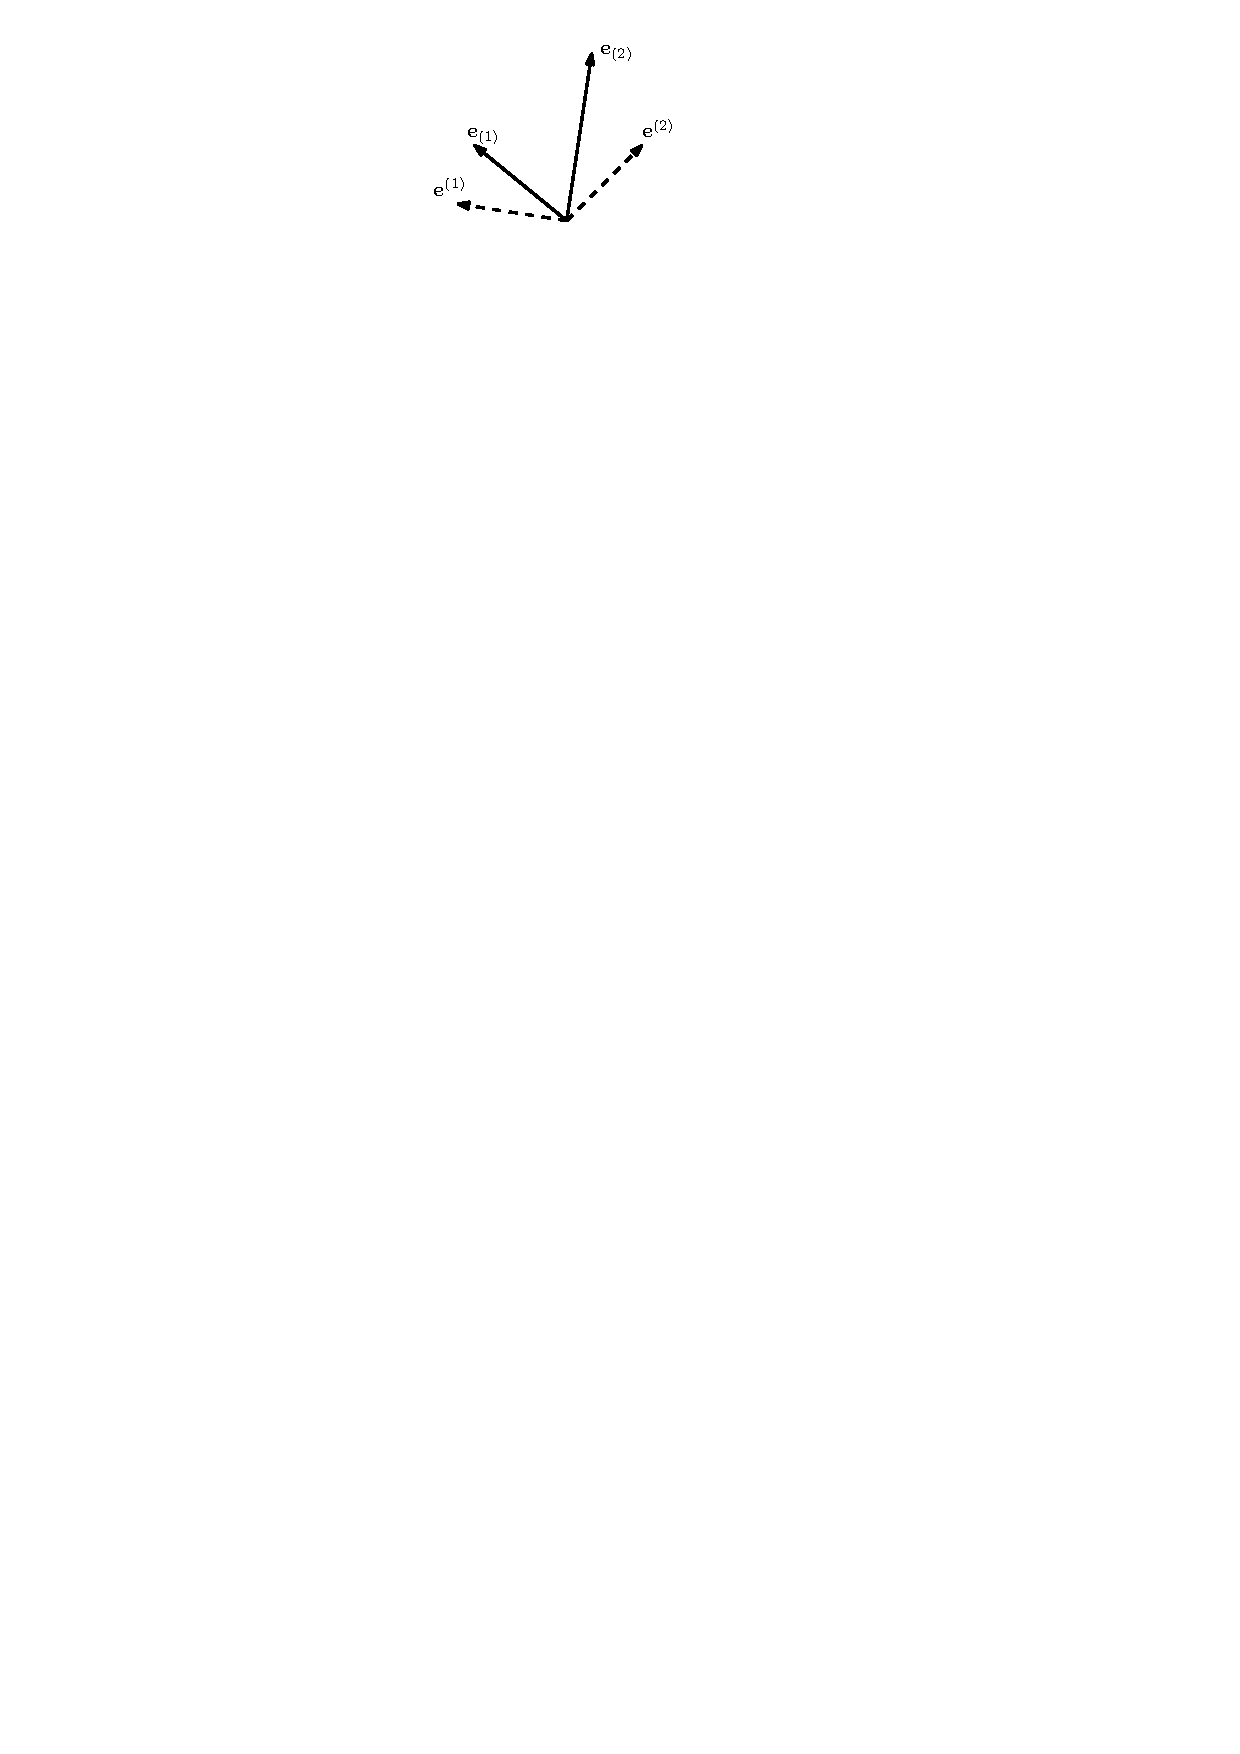
\includegraphics[scale=1.1]{Kap5/tetrads.pdf}\caption{Starting from the two vectors $\left(\boldsymbol{e}_{(1)},\boldsymbol{e}_{(2)}\right)$,
we construct a new vectors $\left(\boldsymbol{e}^{(1)},\boldsymbol{e}^{(2)}\right)$
such that $\boldsymbol{e}_{(1)}\cdot\boldsymbol{e}^{(2)}=0$, $\boldsymbol{e}_{(2)}\cdot\boldsymbol{e}^{(1)}=0$,
$\boldsymbol{e}_{(1)}\cdot\boldsymbol{e}^{(1)}=0$ and $\boldsymbol{e}_{(2)}\cdot\boldsymbol{e}^{(2)}=0$. Traced image from \cite{Alcubierre}\label{fig:tetrads}}
\end{figure}

We will not define yet the values of $\eta_{(a)(b)}$, we will only
say that are constant. The inverse of $\eta_{(a)(b)}$ is defined
in such a way that
\[
\eta_{(a)(b)}\eta^{(b)(c)}=\delta_{(a)}^{(b)},
\]
and as a consequence of the various definitions
\begin{equation}
\eta_{(a)(b)}e_{\alpha}^{(b)}=e_{(b)\alpha},\hspace{1em}\eta^{(a)(b)}e_{(b)\alpha}=e_{\alpha}^{(a)}
\end{equation}
and
\begin{equation}
e_{(a)\alpha}e_{\beta}^{(a)}=g_{\alpha\beta}.\label{eq:g-tetrad}
\end{equation}
A graphical representation of the relation between tetrads is given
in figure \ref{fig:tetrads}.

Given any tensor field, we project it onto the tetrad frame to obtain
its tetrad components. Thus
\begin{align*}
A_{(a)}= & \ e_{(a)\alpha}A^{\alpha}=e_{(a)}^{\alpha}A_{\alpha},\\
A^{(a)}= & \ \eta^{(a)(b)}A_{(b)}=e_{\alpha}^{(a)}A^{\alpha}=e^{(a)\alpha}A_{\alpha},\\
A^{\alpha}= & \ e_{(a)}^{\alpha}A^{(a)}=e^{(a)\alpha}A_{(a)},
\end{align*}
in a more general way we have
\begin{align*}
T_{(a)(b)}= & \ e_{(a)}^{\alpha}e_{(b)}^{\beta}T_{\alpha\beta}=e_{(a)}^{\alpha}T_{\alpha(b)},\\
T_{\alpha\beta}= & \ e_{\alpha}^{(a)}e_{\beta}^{(b)}T_{(a)(b)}=e_{\alpha}^{(a)}T_{(a)\beta}.
\end{align*}

\subsection{Newman-Penrose formalism}

Here we have a special choice of basis vectors, these vectors are
a tetrad $\boldsymbol{l}$, $\boldsymbol{n}$, $\boldsymbol{m}$ and
$\boldsymbol{m}^{*}$, where $\boldsymbol{l}$ and $\boldsymbol{n}$
are real and $\boldsymbol{m}$ and $\boldsymbol{m}^{*}$ are complex
conjugates of one another. These vectors are null and they satisfy
the following orthogonality conditions
\[
\boldsymbol{l}\cdot\boldsymbol{m}=\boldsymbol{l}\cdot\boldsymbol{m}^{*}=\boldsymbol{n}\cdot\boldsymbol{m}=\boldsymbol{n}\cdot\boldsymbol{m}^{*}=0,
\]
besides the requirements
\[
\boldsymbol{l}\cdot\boldsymbol{l}=\boldsymbol{n}\cdot\boldsymbol{n}=\boldsymbol{m}\cdot\boldsymbol{m}=\boldsymbol{m}^{*}\cdot\boldsymbol{m}^{*}=0.
\]
The vectors fulfill the following normalizations conditions
\begin{align*}
\boldsymbol{l}\cdot\boldsymbol{m}= & \ 1,\\
\boldsymbol{m}\cdot\boldsymbol{m}^{*}= & \ -1.
\end{align*}
The constructed vectors are given by
\begin{align}
\boldsymbol{l} & =\frac{1}{\sqrt{2}}\left(\boldsymbol{e}_{(0)}+\boldsymbol{e}_{(1)}\right)\label{eq:tetrad-l}\\
\boldsymbol{n} & =\frac{1}{\sqrt{2}}\left(\boldsymbol{e}_{(0)}-\boldsymbol{e}_{(1)}\right)\label{eq:tetrad-n}\\
\boldsymbol{m} & =\frac{1}{\sqrt{2}}\left(\boldsymbol{e}_{(2)}+i\boldsymbol{e}_{(3)}\right)\label{eq:tetrad-m}\\
\boldsymbol{m}^{*} & =\frac{1}{\sqrt{2}}\left(\boldsymbol{e}_{(2)}-i\boldsymbol{e}_{(3)}\right)\label{eq:tetrad-m2}
\end{align}

For $\eta_{(a)(b)}$, is defined in such a way that
\[
\eta_{(a)(b)}=\eta^{(a)(b)}=\left(\begin{array}{cccc}
0 & -1 & 0 & 0\\
-1 & 0 & 0 & 0\\
0 & 0 & 0 & 1\\
0 & 0 & 1 & 0
\end{array}\right).
\]
The four vectors $\left(\boldsymbol{l},\boldsymbol{n},\boldsymbol{m},\boldsymbol{m}^{*}\right)$
form what is known as a null tetrad. Using (\ref{eq:g-tetrad})
\[
g_{\alpha\beta}=-l_{\alpha}n_{\beta}-n_{\alpha}l_{\beta}+m_{\alpha}m_{\beta}^{*}+m_{\alpha}^{*}m_{\beta}.
\]

\section{The Weyl tensor}

The Weyl tensor for a 4 dimensional manifold is defined as
\[
C_{\alpha\beta\gamma\delta}=R_{\alpha\beta\gamma\delta}-\frac{1}{2}\left(g_{\alpha\gamma}R_{\beta\delta}+g_{\beta\delta}R_{\alpha\gamma}-g_{\beta\gamma}R_{\alpha\delta}-g_{\alpha\delta}R_{\beta\gamma}\right)+\frac{1}{6}R\left(g_{\alpha\gamma}g_{\beta\delta}-g_{\beta\gamma}g_{\alpha\delta}\right).
\]
All contractions of the Weyl tensor vanish identically,
\[
C_{\beta\alpha\delta}^{\alpha}=0,
\]
while its index symmetries are identically to those of the Riemann
tensor,
\[
\begin{array}{l}
C_{\alpha\beta\gamma\delta}=-C_{\beta\alpha\gamma\delta}=C_{\alpha\beta\delta\gamma}=C_{\gamma\delta\alpha\beta},\\
C_{\alpha\beta\gamma\delta}+C_{\alpha\beta\gamma\delta}+C_{\alpha\beta\gamma\delta}=0.
\end{array}
\]
We can write it in its tetrad components
\begin{align*}
C_{(a)(b)(c)(d)}= & \ R_{(a)(b)(c)(d)}+\frac{1}{2}\left(\eta_{(a)(c)}R_{(b)(d)}-\eta_{(b)(c)}R_{(a)(d)}-\eta_{(a)(d)}R_{(b)(c)}+\eta_{(b)(d)}R_{(a)(c)}\right)\\
\  & \ +\frac{1}{6}\left(\eta_{(a)(c)}\eta_{(b)(d)}-\eta_{(a)(d)}\eta_{(b)(c)}\right),
\end{align*}
in the Newman-Penrose formalism, the ten independent components of
the Weyl tensor are represented by the five complex scalars
\begin{align}
\Psi_{0}= & \ C_{(0)(2)(0)(2)}=C_{\alpha\beta\gamma\delta}l^{\alpha}m^{\beta}l^{\gamma}m^{\delta}\\
\Psi_{1}= & \ C_{(0)(1)(0)(2)}=C_{\alpha\beta\gamma\delta}l^{\alpha}n^{\beta}l^{\gamma}m^{\delta}\\
\Psi_{2}= & \ C_{(0)(2)(3)(1)}=C_{\alpha\beta\gamma\delta}l^{\alpha}m^{\beta}m^{*\gamma}n^{\delta}\\
\Psi_{3}= & \ C_{(1)(2)(3)(2)}=C_{\alpha\beta\gamma\delta}l^{\alpha}n^{\beta}m^{*\gamma}n^{\delta}\\
\Psi_{4}= & \ C_{(1)(3)(1)(3)}=C_{\alpha\beta\gamma\delta}n^{\alpha}m^{*\beta}n^{\gamma}m^{*\delta},\label{eq:psi4}
\end{align}
this scalars are useful, in particular $\Psi_{4}$, for the radiated
energy and momentum expressions.

\subsection{Radiated energy and momentum}

Let us define the complex quantity $H$ such that
\[
H=h^{+}-ih^{\times},
\]
we can write the average
\[
\left\langle \left(\partial_{t}h^{+}\right)^{2}+\left(\partial_{t}h^{\times}\right)^{2}\right\rangle 
\]
in terms of $H$. We have that
\[
\partial_{\alpha}H\partial_{\beta}H^{*}=\left[\partial_{\alpha}h^{+}\partial_{\beta}h^{+}+\partial_{\alpha}h^{\times}\partial_{\beta}h^{\times}\right]+i\left[\partial_{\alpha}h^{+}\partial_{\beta}h^{\times}-\partial_{\alpha}h^{\times}\partial_{\beta}h^{+}\right],
\]
we take the following case
\[
\partial_{t}H\partial_{r}H^{*}=\left[\partial_{t}h^{+}\partial_{r}h^{+}+\partial_{t}h^{\times}\partial_{r}h^{\times}\right]+i\left[\partial_{t}h^{+}\partial_{r}h^{\times}-\partial_{t}h^{\times}\partial_{r}h^{+}\right],
\]
then
\begin{equation}
\text{Re}\left(\partial_{t}H\partial_{r}H^{*}\right)=\partial_{t}h^{+}\partial_{r}h^{+}+\partial_{t}h^{\times}\partial_{r}h^{\times},\label{eq:reh}
\end{equation}
where $\text{Re}\left(\cdots\right)$ is the real part of a complex
number. In the second chapter we show that $\partial_{r}h_{ij}^{TT}\left(t,r\right)\approx-\partial_{0}h_{ij}^{TT}\left(t,r\right)$
in the radiation zone, therefore
\begin{align*}
\left\langle \partial_{t}H\partial_{r}H^{*}\right\rangle = & \ \left\langle \partial_{t}H\partial_{t}H^{*}\right\rangle \\
= & \ \left\langle \left|\partial_{t}H\right|^{2}\right\rangle 
\end{align*}
and from (\ref{eq:reh})
\[
\left\langle \left|\partial_{t}H\right|^{2}\right\rangle =\left\langle \left(\partial_{t}h^{+}\right)^{2}+\left(\partial_{t}h^{\times}\right)^{2}\right\rangle .
\]
This allow us to write equation (\ref{eq:dedt-ch2}) as
\[
\frac{dE}{dt}=\frac{c^{3}r^{2}}{16\pi G}\int\left\langle \left|\partial_{t}H\right|^{2}\right\rangle d\Omega.
\]

We construct a null tetrad from the orthonormal spherical basis using
the equations (\ref{eq:tetrad-l}), (\ref{eq:tetrad-n}), (\ref{eq:tetrad-m})
and (\ref{eq:tetrad-m2})
\begin{align*}
l^{\alpha}:= & \frac{1}{\sqrt{2}}\left(e_{t}^{\alpha}+e_{r}^{\alpha}\right),\\
n^{\alpha}:= & \frac{1}{\sqrt{2}}\left(e_{t}^{\alpha}-e_{r}^{\alpha}\right),\\
m^{\alpha}:= & \frac{1}{\sqrt{2}}\left(e_{\theta}^{\alpha}+ie_{\phi}^{\alpha}\right),\\
m^{*\alpha}:= & \frac{1}{\sqrt{2}}\left(e_{\theta}^{\alpha}-ie_{\phi}^{\alpha}\right),
\end{align*}
where the vectors $\boldsymbol{e}_{t}$, $\boldsymbol{e}_{r}$,
$\boldsymbol{e}_{\theta}$ and $\boldsymbol{e}_{\phi}$ are the
usual orthonormal basis induced by the spherical coordinates. Calculating
$\Psi_{4}$ from equation (\ref{eq:psi4}) and the null tetrad constructed
above, knowing that there is no explicit dependence of $t$, $\theta$
and $\phi$ we obtain that
\[
\Psi_{4}=-\frac{1}{4}\left(\partial_{t}^{2}h^{+}-2\partial_{t}\partial_{r}h^{+}+\partial_{r}^{2}h^{+}\right)+\frac{i}{4}\left(\partial_{t}^{2}h^{\times}-2\partial_{t}\partial_{r}h^{\times}+\partial_{r}^{2}h^{\times}\right),
\]
given that we are in the local wave zone then $\partial_{r}h=-\partial_{0}h$,
therefore
\[
\Psi_{4}=-\partial_{t}^{2}h^{+}+i\partial_{t}^{2}h^{\times}=-\partial_{t}^{2}H.
\]
This implies that for outgoing gravitational waves we can write
\begin{equation}
H=-\int_{-\infty}^{t}\int_{-\infty}^{t'}\Psi_{4}dt''dt',\label{eq:h-psi4}
\end{equation}
then the total flux energy leaving the system is
\[
\frac{dE}{dt}=\frac{c^{3}r^{2}}{16\pi G}\int\left|\int_{-\infty}^{t}\Psi_{4}dt'\right|^{2}d\Omega.
\]

Now we are going to write the flux of momentum along the radial direction,
this expression is given in Chapter \ref{chp2}, writing it in term of $H$ we
have that
\[
\frac{dP_{i}}{dt}=\frac{c^{3}r^{2}}{16\pi G}\int k_i\left|\partial_{t}H\right|^{2}d\Omega
\]
where
\[
k_i=\frac{\boldsymbol{x}}{r}=\left(\sin\theta\cos\varphi,\sin\theta\sin\varphi,\cos\theta\right),
\]
for this it was used the fact that in the wave zone the angular dependence can be neglected, then $\partial_iH=\left(x_i/r\right)\partial_rH$ and that $\partial_{r}h=-\partial_{0}h$. Then, from (\ref{eq:h-psi4}) we finally got
\[
\frac{dP_{i}}{dt}=\frac{c^{3}r^{2}}{16\pi G}\int k_i\left|\int_{-\infty}^{t}\Psi_{4}dt'\right|^{2}d\Omega.
\]

Now we are going to calculate the flux of angular momentum, we are
going to calculate it from the expression (\ref{eq:an-mom-flux}). We are going
to rewrite this expression introducing the angular vectors $\boldsymbol{\xi}_{i}$
associated to rotations around the three coordinate axis. These vectors
are Killing fields of the flat metric, and in Cartesian coordinates
have components given by $\xi_{i}^{k}=\epsilon_{i}^{jk}x_{j}$\footnote{This can be view from the general solution of the Killing equation
in flat spacetime, from eq. (\ref{eq:killing-general}) we take $a_{\alpha}=0$ and
particular values for $l_{\alpha\beta}$ such that we obtain this
form of the vector.}, where $\xi_{i}^{k}$ represents the $k$ component of the vector
$\boldsymbol{\xi}_{i}$. Let us write the flux of angular momentum
in terms of the Lie derivative, for this we are going to use the expression
\begin{equation}
\left(\mathcal{L}_{\boldsymbol{\xi}_{i}}\boldsymbol{h}\right)_{\alpha\beta}=\xi_{i}^{\sigma}\partial_{\sigma}h_{\alpha\beta}+h_{\sigma\beta}\partial_{\alpha}\xi_{i}^{\sigma}+h_{\alpha\sigma}\partial_{\beta}\xi_{i}^{\sigma},\label{eq:lie-wav}
\end{equation}
given that we are in the local wave zone we restrict ourselves to
the index $a,b,c,...$ where these run from 1 to 2. If we multiply
(\ref{eq:lie-wav}) by $\partial_{r}h^{ab}$ and sum over $a$ and
$b$, because $\boldsymbol{\xi}_{i}$ is a Killing vector then
\[
h_{cb}\partial_{a}\xi_{i}^{c}\partial_{r}h^{ab}+h_{ac}\partial_{b}\xi_{i}^{c}\partial_{r}h^{ab}=0,
\]
and because we are in the gauge TT the term $\left(2\delta_{aj}\epsilon_{i}^{jk}h_{bj}\right)\partial_{r}h^{ab}=0.$
Then we can write the flux of angular momentum as
\begin{equation}
\frac{dJ_{i}}{dt}=-\frac{c^{3}r^{2}}{32\pi G}\int\left(\mathcal{L}_{\boldsymbol{\xi}_{i}}\boldsymbol{h}\right)_{ab}\partial_{r}h^{ab}d\Omega.\label{eq:djdt-lie}
\end{equation}
Now we want to write (\ref{eq:djdt-lie}) in terms of $H$, for this
we are going to introduce spherical coordinates $(r,\theta,\varphi)$,
this implies that
\begin{align*}
\boldsymbol{\xi}_{x}= & \ \left(0,-\sin\varphi,-\cos\varphi\cot\theta\right)\\
\boldsymbol{\xi}_{y}= & \ \left(0,\cos\varphi,-\sin\varphi\cot\theta\right)\\
\boldsymbol{\xi}_{z}= & \ \left(0,0,1\right),
\end{align*}
because along $\boldsymbol{\xi}_{z}$ the Lie derivatives reduce to
partial derivatives, we are going to introduce two angular vectors
to calculate the Lie derivatives in the other directions

\begin{align*}
\boldsymbol{\xi}_{\pm}= & \ \boldsymbol{\xi}_{x}\pm i\boldsymbol{\xi}_{y}\\
= & \ e^{\pm i\varphi}\left(0,\pm i,-\cot\theta\right).
\end{align*}
Let us also introduce an orthonormal spherical basis $(\boldsymbol{e}_{r},\boldsymbol{e}_{\theta},\boldsymbol{e}_{\varphi})$
and two unit complex vectors
\begin{align*}
\boldsymbol{e}_{\pm}= & \ \frac{1}{\sqrt{2}}\left(\boldsymbol{e}_{\theta}\pm i\boldsymbol{e}_{\varphi}\right)\\
= & \ \frac{1}{r\sqrt{2}}\left(0,1,\mp i\csc\theta\right).
\end{align*}

Let us calculate the Lie derivative of $\boldsymbol{e}_{\pm}$ along
$\boldsymbol{\xi}_{\pm}$, because these are vectors we calculate
the Lie derivative with the Lie brackets
\begin{align*}
\mathcal{L}_{\boldsymbol{\xi}_{\pm}}\boldsymbol{e}_{\pm}= & \ \left[\boldsymbol{\xi}_{\pm},\boldsymbol{e}_{\pm}\right]\\
= & \ \left[\pm ie^{\pm i\varphi}\partial_{\theta}-e^{\pm i\varphi}\cot\theta\partial_{\varphi}\right]\left(\frac{1}{r\sqrt{2}}\partial_{\theta}\mp\frac{i}{r\sqrt{2}}\csc\theta\right)\\
\  & \ -\left[\frac{1}{r\sqrt{2}}\partial_{\theta}\mp\frac{i}{r\sqrt{2}}\csc\theta\partial_{\varphi}\right]\left(\pm ie^{\pm i\varphi}\partial_{\theta}-e^{\pm i\varphi}\cot\theta\partial_{\varphi}\right),
\end{align*}
calculating the derivatives and factoring we have
\[
\left(\mathcal{L}_{\boldsymbol{\xi}_{\pm}}\boldsymbol{e}_{\pm}\right)^{a}=\mp\left(ie^{\pm i\varphi}\csc\theta\right)\left(\boldsymbol{e}_{\pm}\right)^{a}.
\]

Now we write the linearized field $h_{ab}$ in the TT gauge in terms
of the orthonormal basis
\begin{align*}
h_{ab}= & \ h^{+}\left[\left(\boldsymbol{e}_{\theta}\right)_{a}\left(\boldsymbol{e}_{\theta}\right)_{b}-\left(\boldsymbol{e}_{\varphi}\right)_{a}\left(\boldsymbol{e}_{\varphi}\right)_{b}\right]+h^{\times}\left[\left(\boldsymbol{e}_{\theta}\right)_{a}\left(\boldsymbol{e}_{\varphi}\right)_{b}-\left(\boldsymbol{e}_{\varphi}\right)_{a}\left(\boldsymbol{e}_{\theta}\right)_{b}\right]\\
= & \ \left(h^{+}-ih^{\times}\right)\left(\boldsymbol{e}_{-}\right)_{a}\left(\boldsymbol{e}_{-}\right)_{b}+\left(h^{+}+ih^{\times}\right)\left(\boldsymbol{e}_{+}\right)_{a}\left(\boldsymbol{e}_{+}\right)_{b}\\
= & \ H\left(\boldsymbol{e}_{-}\right)_{a}\left(\boldsymbol{e}_{-}\right)_{b}+\bar{H}\left(\boldsymbol{e}_{+}\right)_{a}\left(\boldsymbol{e}_{+}\right)_{b},
\end{align*}
with this we have
\begin{align*}
\left(\mathcal{L}_{\boldsymbol{\xi}_{\pm}}\boldsymbol{h}\right)_{ab}= & \ H\left[\left(\mathcal{L}_{\boldsymbol{\xi}_{\pm}}\boldsymbol{e}_{-}\right)_{a}\left(\boldsymbol{e}_{-}\right)_{b}+\left(\boldsymbol{e}_{-}\right)_{a}\left(\mathcal{L}_{\boldsymbol{\xi}_{\pm}}\boldsymbol{e}_{-}\right)_{b}\right]+\bar{H}\left[\left(\mathcal{L}_{\boldsymbol{\xi}_{\pm}}\boldsymbol{e}_{+}\right)_{a}\left(\boldsymbol{e}_{+}\right)_{b}+\left(\boldsymbol{e}_{+}\right)_{a}\left(\mathcal{L}_{\boldsymbol{\xi}_{\pm}}\boldsymbol{e}_{+}\right)_{b}\right]\\
= & \ -2ie^{\pm i\varphi}\csc\theta\left(\boldsymbol{e}_{-}\right)_{a}\left(\boldsymbol{e}_{-}\right)_{b}H+2ie^{\pm i\varphi}\csc\theta\left(\boldsymbol{e}_{-}\right)_{a}\left(\boldsymbol{e}_{-}\right)_{b}\bar{H}.
\end{align*}
Let us define the following operators
\[
\hat{J}_{\pm}=\xi_{\pm}^{a}\partial_{a}-ise^{\pm i\varphi}\csc\theta=e^{\pm i\varphi}\left(\pm i\partial_{\theta}-\cot\theta\partial_{\varphi}-is\csc\theta\right),
\]
where $s$ is known as the spin weight of the function\footnote{For details of the general theory where the spin weight of a function
is used see \cite{Alcubierre} Appendix D}, $s=-2$ for $H$ and $s=2$ for $\bar{H}$, then
\[
\left(\mathcal{L}_{\boldsymbol{\xi}_{\pm}}\boldsymbol{h}\right)_{ab}=\left(\boldsymbol{e}_{-}\right)_{a}\left(\boldsymbol{e}_{-}\right)_{b}\hat{J}_{\pm}H+\left(\boldsymbol{e}_{+}\right)_{a}\left(\boldsymbol{e}_{+}\right)_{b}\hat{J}_{\pm}\bar{H}.
\]
Calculating $\left(\mathcal{L}_{\boldsymbol{\xi}_{\pm}}\boldsymbol{h}\right)_{ab}\partial_{t}h^{ab}$
\begin{align*}
\left(\mathcal{L}_{\boldsymbol{\xi}_{\pm}}\boldsymbol{h}\right)_{ab}\partial_{t}h^{ab}= & \ \left[\left(\boldsymbol{e}_{-}\right)_{a}\left(\boldsymbol{e}_{-}\right)_{b}\hat{J}_{\pm}H+\left(\boldsymbol{e}_{+}\right)_{a}\left(\boldsymbol{e}_{+}\right)_{b}\hat{J}_{\pm}\bar{H}.\right]\partial_{t}\left[H\left(\boldsymbol{e}_{-}\right)_{a}\left(\boldsymbol{e}_{-}\right)_{b}+\bar{H}\left(\boldsymbol{e}_{+}\right)_{a}\left(\boldsymbol{e}_{+}\right)_{b}\right],
\end{align*}
because $\boldsymbol{e}_{\theta}$ and $\boldsymbol{e}_{\varphi}$
are orthogonal $\left(\boldsymbol{e}_{-}\right)_{a}\left(\boldsymbol{e}_{-}\right)^{a}=\left(\boldsymbol{e}_{+}\right)_{b}\left(\boldsymbol{e}_{+}\right)^{b}=0$
and $\left(\boldsymbol{e}_{-}\right)_{a}\left(\boldsymbol{e}_{+}\right)^{a}=\left(\boldsymbol{e}_{+}\right)_{b}\left(\boldsymbol{e}_{-}\right)^{b}=1$,
therefore
\begin{equation}
\left(\mathcal{L}_{\boldsymbol{\xi}_{\pm}}\boldsymbol{h}\right)_{ab}\partial_{t}h^{ab}=\hat{J}_{\pm}H\partial_{t}\bar{H}+\hat{J}_{\pm}\bar{H}\partial_{t}H=2\text{Re}\left\{ \hat{J}_{\pm}H\partial_{t}\bar{H}\right\} .\label{eq:lehj}
\end{equation}
From (\ref{eq:lehj}) and the properties of the Lie derivative
\begin{align}
\hat{J}_{+}H\partial_{t}\bar{H}+\hat{J}_{+}\bar{H}\partial_{t}H= & \ \left(\mathcal{L}_{\boldsymbol{\xi}_{x}}\boldsymbol{h}+i\mathcal{L}_{\boldsymbol{\xi}_{y}}\boldsymbol{h}\right)_{ab}\partial_{t}h_{ab}\label{eq:jh+}\\
\hat{J}_{-}H\partial_{t}\bar{H}+\hat{J}_{-}\bar{H}\partial_{t}H= & \ \left(\mathcal{L}_{\boldsymbol{\xi}_{x}}\boldsymbol{h}-i\mathcal{L}_{\boldsymbol{\xi}_{y}}\boldsymbol{h}\right)_{ab}\partial_{t}h_{ab}\label{eq:jh-}
\end{align}
then making (\ref{eq:jh+})+(\ref{eq:jh-}) and (\ref{eq:jh+})-(\ref{eq:jh-}),
and defining the operators
\begin{align*}
\hat{J}_{x}= & \ \frac{\hat{J}_{+}+\hat{J}_{-}}{2} & \hat{J}_{y}= & \ \frac{\hat{J}_{+}-\hat{J}_{-}}{2}
\end{align*}
we have
\begin{align}
\left(\mathcal{L}_{\boldsymbol{\xi}_{x}}\boldsymbol{h}\right)_{ab}\partial_{t}h_{ab}= & \ \hat{J}_{x}H\partial_{t}\bar{H}+\hat{J}_{x}\bar{H}\partial_{t}H=2\text{Re}\left\{ \hat{J}_{x}H\partial_{t}\bar{H}\right\} \label{eq:jx}\\
\left(\mathcal{L}_{\boldsymbol{\xi}_{y}}\boldsymbol{h}\right)_{ab}\partial_{t}h_{ab}= & \ \hat{J}_{y}H\partial_{t}\bar{H}+\hat{J}_{y}\bar{H}\partial_{t}H=2\text{Re}\left\{ \hat{J}_{y}H\partial_{t}\bar{H}\right\} .\label{eq:jy}
\end{align}
From (\ref{eq:jx}) and (\ref{eq:jy}) we write (\ref{eq:djdt-lie})
as
\[
\frac{dJ_{i}}{dt}=\frac{c^{3}r^{2}}{16\pi G}\text{Re}\left\{ \int\hat{J}_{i}H\partial_{t}\bar{H}d\Omega\right\} ,
\]
because (\ref{eq:h-psi4})
\[
\frac{dJ_{i}}{dt}=-\frac{c^{3}r^{2}}{16\pi G}\text{Re}\left\{ \int\left[\left(\int_{-\infty}^{t}\bar{\Psi}_{4}dt'\right)\hat{J}_{i}\left(\int_{-\infty}^{t''}\int_{-\infty}^{t'}\Psi_{4}dt''dt'\right)\right]d\Omega\right\} .
\]
Therefore we obtained the flux of energy, linear and angular momentum
for the gravitational radiation in terms of the Weyl scalar $\Psi_{4}$.
\begin{figure}[h]
	\centering{}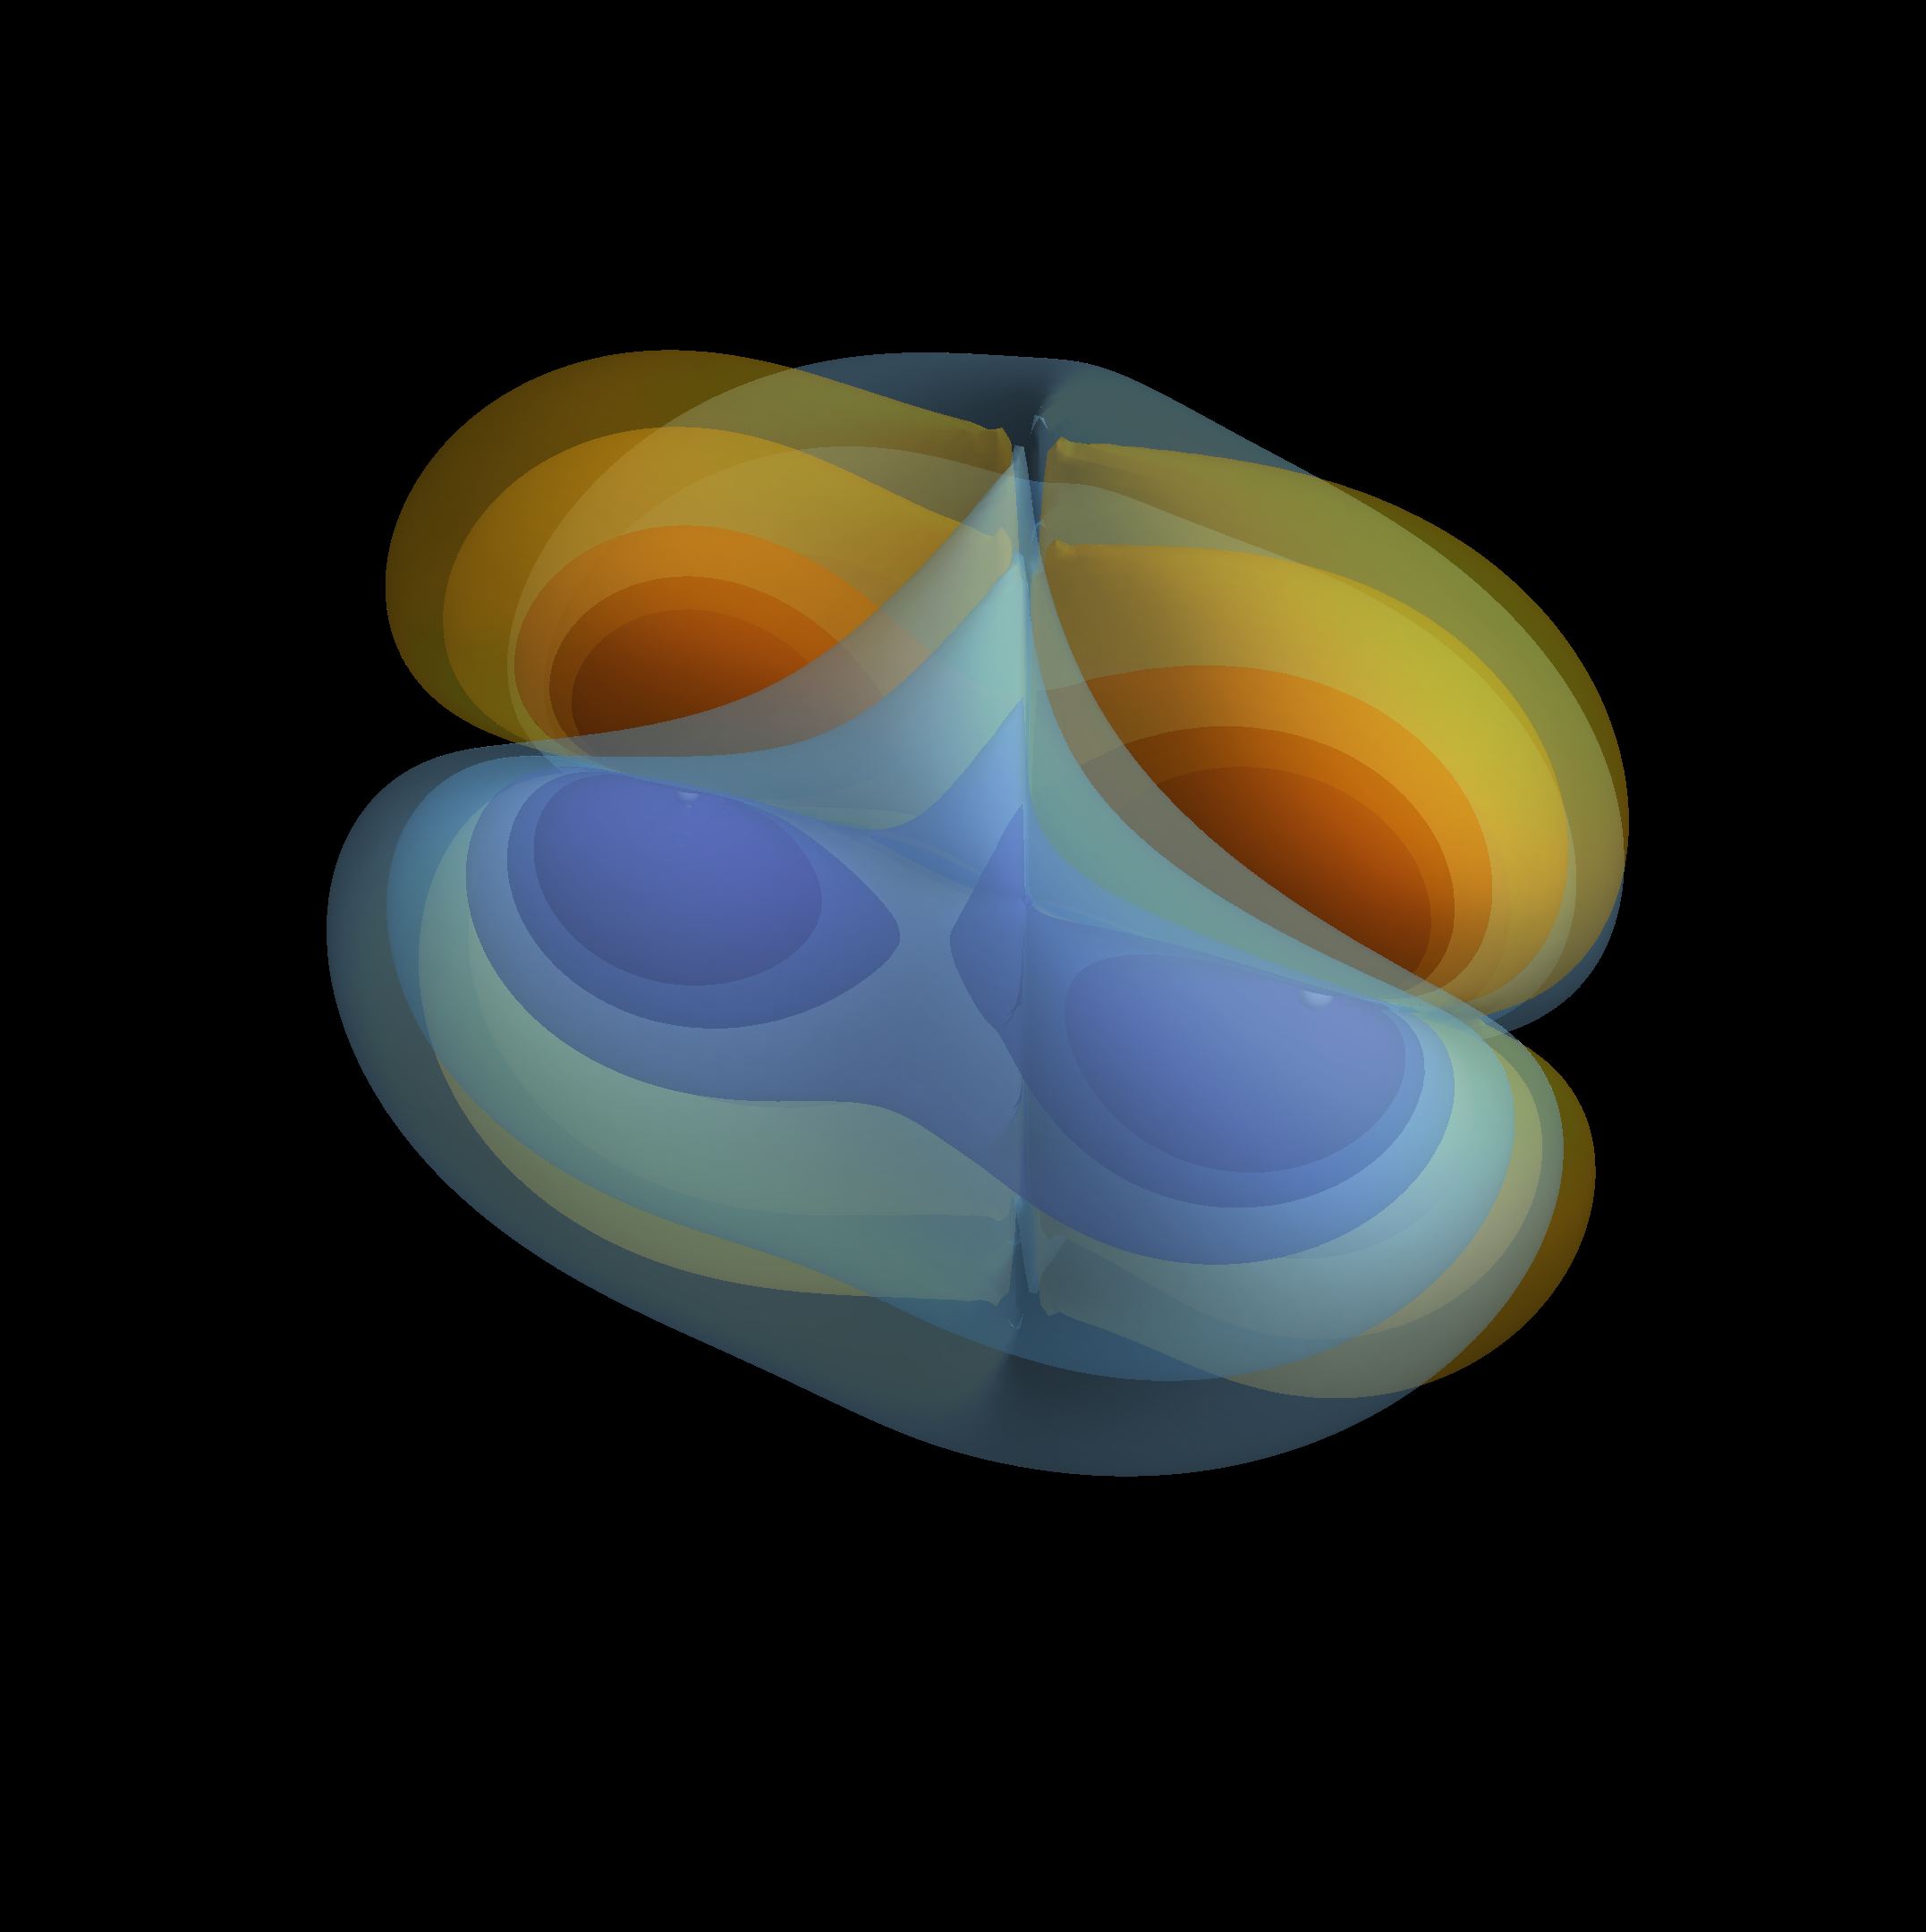
\includegraphics[scale=0.12]{Kap5/RePsi4.png}\caption{Real part of $\Psi_4$ representing outgoing gravitational radiation. Image taken from \textit{https://einsteintoolkit.org} \label{fig:psi4}}
\end{figure}
The importance of the Weyl scalar is seen in Figure \ref{fig:psi4}. This is a simulation of \textit{Einstein toolkit} code. Is made for a merger 36 + 29 solar mass binary black hole system. It is the $\Psi_4$ real part contribution of outgoing radiation in the wave zone. From this scalar we can characterize somehow the astrophysical systems and help to identify some aspects of them, for example, in gravitational collapse there is no gravitational radiation, this is because the Weyl tensor in this system is zero, therefore $\Psi_4=0$. For details see \cite{GRAVITATION}. 



%\chapter{Conclusions and recommendations}
\section{Conclusions}
It was understood the radiation conditions for the linearized gravity, this includes the comparison of the radiation zone in electrodynamics and in linearized gravity, the role of the background and physical manifold, how gauge transformations works and the energy contribution of gravitational radiation and the study of the characteristic length of the background and the radiation. The function of manifolds in gravitational radiation is usually omitted, just like why the energy has to be average and how it can be average. Gauge transformations are not usually study from the point of view of the diffeomorphism between manifolds and the characteristic length is usually just mention. The general equation for the study of gravitational radiation was deduced and the expressions of energy, lineal and angular momentum where obtained. Finally the contribution of the Weyl tensor in gravitational radiation was highlighted, this role is really important for the generation of gravitational radiation for astrophysical systems.
\section{Recommendations}
The idea is to apply this theory into an astrophysical system, be able to calculate the energy contribution of this system, and even try to simulate it. Make a comparison between a simulation made from linearized gravity point of view and the relaxed Einstein field equations, so it can be check at which point linearized gravity is a good approximation and study the Weyl tensor contribution for this system. There exists codes which helps in the analysis of this systems, a particular one is \textit{Einstein Toolkit}\footnote{Einstein Toolkit website: https//einsteintoolkit.org}, which use numerical relativity for its simulations. The study of this kind of codes could improve the knowledge in gravitational radiation for astrophysical systems.\\
%\begin{appendix}
\chapter{Appendix A: Harmonic coordinates}\label{appendix-harm}
In this appendix first we will proof some properties of the Christoffel symbols and the metric tensor components. Then these properties are going to be
use to arrived, from the harmonic coordinates, to the DeDonder gauge.
Main reference for this appendix is \cite{DIRAC}.

\section{Useful properties}

The following properties are going to be useful for this appendix

\subsection*{Property 1}

\begin{equation}
\partial_{\sigma}g^{\alpha\beta}=-g^{\alpha\mu}g^{\beta\nu}\partial_{\sigma}g_{\mu\nu},\label{eq:a1}
\end{equation}
\textbf{Proof:} We start from
\begin{align*}
\partial_{\sigma}g^{\alpha\mu}\cdot g_{\mu\nu}+g^{\alpha\mu}\cdot\partial_{\sigma}g_{\mu\nu} & =\partial_{\sigma}\left(g^{\alpha\mu}g_{\mu\nu}\right)\\
\  & =\partial_{\sigma}\delta_{\nu}^{\alpha}\\
\  & =0
\end{align*}
then
\[
\partial_{\sigma}g^{\alpha\mu}\cdot g_{\mu\nu}=-g^{\alpha\mu}\cdot\partial_{\sigma}g_{\mu\nu},
\]
multiplying by $g^{\beta\nu}$ and adding in $\nu$, because $g^{\beta\nu}g_{\mu\nu}=\delta_{\mu}^{\beta}$,
we obtain (\ref{eq:a1}).

\subsection*{Property 2}

\begin{equation}
\Gamma_{\alpha\beta\sigma}+\Gamma_{\beta\alpha\sigma}=\partial_{\sigma}g_{\alpha\beta},\label{eq:a2}
\end{equation}
\textbf{Proof:} From the fact that
\[
\Gamma_{\beta\gamma}^{\alpha}=\frac{1}{2}g^{\alpha\sigma}\left(\partial_{\beta}g_{\sigma\gamma}+\partial_{\gamma}g_{\sigma\beta}-\partial_{\sigma}g_{\beta\gamma}\right)
\]
we have that
\[
\Gamma_{\alpha\beta\sigma}=\frac{1}{2}\left(\partial_{\beta}g_{\alpha\sigma}+\partial_{\sigma}g_{\alpha\beta}-\partial_{\alpha}g_{\beta\sigma}\right)
\]
and

\[
\Gamma_{\beta\alpha\sigma}=\frac{1}{2}\left(\partial_{\alpha}g_{\beta\sigma}+\partial_{\sigma}g_{\beta\alpha}-\partial_{\beta}g_{\alpha\sigma}\right),
\]
if we make $\Gamma_{\alpha\beta\sigma}+\Gamma_{\beta\alpha\sigma}$
we obtain (\ref{eq:a2}).

\subsection*{Property 3}

\begin{equation}
\Gamma_{\alpha\beta}^{\beta}\sqrt{-g}=\partial_{\text{\ensuremath{\alpha}}}\sqrt{-g},\label{eq:a3}
\end{equation}
\textbf{Proof: }First we have to differentiate the determinant of
the metric tensor $g$, we must differentiate each element $g_{\lambda\mu}$
in it and then multiply by the cofactor $gg^{\lambda u}$. Thus
\begin{equation}
\partial_{\nu}g=gg^{\lambda\mu}\partial_{\nu}g_{\lambda\mu}.\label{eq:ag}
\end{equation}
Now we are going to calculate $\Gamma_{\nu\mu}^{\mu}$
\begin{align}
\Gamma_{\nu\mu}^{\mu} & =\frac{1}{2}g^{\mu\sigma}\left(\partial_{\mu}g_{\sigma\nu}+\partial_{\nu}g_{\sigma\mu}-\partial_{\sigma}g_{\nu\mu}\right)\\
\  & =\frac{1}{2}\left(g^{\mu\sigma}\partial_{\mu}g_{\sigma\nu}-g^{\mu\sigma}\partial_{\sigma}g_{\nu\mu}+g^{\mu\sigma}\partial_{\nu}g_{\sigma\mu}\right)\\
\  & =\frac{1}{2}g^{\mu\sigma}\partial_{\nu}g_{\sigma\mu}.\label{eq:a-gamma}
\end{align}
Let us write $g^{-1}\partial_{\nu}g$ in the following way
\begin{align}
g^{-1}\partial_{\nu}g & =g^{-1}\partial_{\nu}\left(\left[\sqrt{-g}\right]^{2}\right)\nonumber \\
\  & =2\left(\sqrt{-g}\right)^{-1}\partial_{\nu}\sqrt{-g},\label{eq:a-sqrt}
\end{align}
from (\ref{eq:ag}) and (\ref{eq:a-sqrt})
\begin{equation}
\partial_{\nu}\sqrt{-g}=\frac{1}{2}\sqrt{-g}g^{\lambda\mu}\partial_{\nu}g_{\lambda\mu}.\label{eq:a-gg}
\end{equation}
Using (\ref{eq:a-gg}) in (\ref{eq:a-gamma}) we obtain (\ref{eq:a3}).

\section{The DeDonder Gauge}

To understand harmonic coordinates we have to start from the d'Alembert
equation for a scalar $V$, namely $\boxempty V=0$, in a curved spacetime
\[
\boxempty V=g^{\alpha\beta}\nabla_{\alpha}\nabla_{\beta}V,
\]
then
\[
g^{\alpha\beta}\nabla_{\alpha}\nabla_{\beta}V=g^{\alpha\beta}\nabla_{\alpha}\left(\partial_{\beta}V\right)=g^{\alpha\beta}\left(\partial_{\alpha}\partial_{\beta}V-\Gamma_{\alpha\beta}^{\sigma}\partial_{\sigma}V\right)=0,
\]
if we are using rectilinear axes in flat space, each of the four coordinates
$x^{\alpha}$ satisfies $\boxempty x^{\alpha}=0$. This impose a restriction
over the coordinates, because $x^{\alpha}$ is not an scalar like
$V$, so it holds only in certain coordinate system.

If we substitute $x^{\alpha}$ for $V$
\begin{align*}
g^{\alpha\beta}\left(\partial_{\alpha}\partial_{\beta}x^{\lambda}-\Gamma_{\alpha\beta}^{\sigma}\partial_{\sigma}x^{\lambda}\right)= & \ g^{\alpha\beta}\left(\partial_{\alpha}\delta_{\text{\ensuremath{\beta}}}^{\lambda}-\Gamma_{\alpha\beta}^{\sigma}\delta_{\text{\ensuremath{\sigma}}}^{\lambda}\right)\\
= & \ -g^{\alpha\beta}\Gamma_{\alpha\beta}^{\lambda}=0,
\end{align*}
the coordinates that satisfies this condition are called \textbf{harmonic
coordinates}. They provide the closest approximation to rectilinear
coordinates that we can have in curved spacetime. Now, we are going
to prove that the harmonic coordinate system is equivalent to set
the DeDonder gauge $\partial_{\beta}\left(g^{\alpha\beta}\sqrt{-g}\right)=0$,
from equations (\ref{eq:a1}) and (\ref{eq:a2})

\begin{align*}
\partial_{\sigma}g^{\alpha\beta}= & \ -g^{\alpha\mu}g^{\beta\nu}\left(\Gamma_{\mu\nu\sigma}+\Gamma_{\nu\mu\sigma}\right)\\
= & \ -g^{\alpha\mu}\Gamma_{\mu\sigma}^{\beta}-g^{\beta\nu}\Gamma_{\nu\sigma}^{\alpha},
\end{align*}
from equation (\ref{eq:a2}) and (\ref{eq:a3}) 
\begin{align*}
\partial_{\sigma}\left(g^{\alpha\beta}\sqrt{-g}\right)= & \ \sqrt{-g}\partial_{\sigma}g^{\alpha\beta}+g^{\alpha\beta}\partial_{\sigma}\sqrt{-g}\\
= & \ \sqrt{-g}\left(-g^{\alpha\mu}\Gamma_{\mu\sigma}^{\beta}-g^{\beta\nu}\Gamma_{\nu\sigma}^{\alpha}+g^{\alpha\beta}\Gamma_{\sigma\mu}^{\mu}\right),
\end{align*}
contracting $\sigma$ and $\beta$
\begin{align*}
\partial_{\beta}\left(g^{\alpha\beta}\sqrt{-g}\right)= & \ \sqrt{-g}\left(-g^{\alpha\mu}\Gamma_{\mu\beta}^{\beta}-g^{\beta\nu}\Gamma_{\nu\beta}^{\alpha}+g^{\alpha\beta}\Gamma_{\beta\mu}^{\mu}\right)\\
= & \ -\sqrt{-g}g^{\beta\nu}\Gamma_{\nu\beta}^{\alpha},
\end{align*}
because $g^{\alpha\beta}\Gamma_{\alpha\beta}^{\lambda}=0$, then
\[
\partial_{\beta}\left(g^{\alpha\beta}\sqrt{-g}\right)=0
\]
which is what we wanted to proof.
%%%%%%%%%%%%%%%%%%%%%%%%%%%%%%%%%%%%%%%%%%%%%%%%%%%%%%%%%%%
\chapter{Appendix B: Relativistic Angular Momentum}\label{appendix-momentum}
In this appendix will be obtain the expression for the relativistic angular momentum for a closed particle system. Then a general system is consider with a general action integral, a momentum and angular momentum expression is obtained and the role of the angular momentum conservation in the symmetry of the energy-momentum tensor. Main reference is \cite{LANDAU,DEWITT}.

\section{For a closed particle system}

Here we are going to obtain a relativistic expression for the angular
momentum. We need to take into account that there is conservation
of angular momentum in classical mechanics, so here we are goint to
take a rotation and proof that there is an expression that is conserved
under rotations in the four-dimensional space and this expression
is the angular momentum. We also verify that this correspond to the
angular momentum expression when we return to a classical system. 

Let us take a system of several particles, let $x^{\alpha}$ be the
coordinates of one of the particles of the system. We make an infinitesimal
rotation in the four-dimensional space. Under a transformation, the
coordinates $x^{\alpha}$ take on new values $x'^{\alpha}$ such that
the differences $x'^{\alpha}-x^{\alpha}$ are linear functions
\begin{equation}
x'^{\alpha}-x^{\alpha}=x_{\beta}\delta\Omega^{\alpha\beta},\label{eq:b1}
\end{equation}
where $\delta\Omega^{\alpha\beta}$ are infinitesimal coefficients.
Under rotation, the length of the four-position vector must remain
unchaged
\begin{equation}
x'_{\alpha}x'^{\alpha}=x_{\alpha}x^{\alpha},\label{eq:b2}
\end{equation}
from equation (\ref{eq:b1}) $x'^{\alpha}=x^{\alpha}+x_{\beta}\delta\Omega^{\alpha\beta}$,
then
\begin{align*}
x'_{\alpha}x'^{\alpha}= & \ \left(x_{\alpha}+x_{\beta}\delta\Omega_{\alpha}^{\beta}\right)\left(x^{\alpha}+x_{\beta}\delta\Omega^{\alpha\beta}\right)\\
= & \ x_{\alpha}x^{\alpha}+x_{\alpha}x_{\beta}\delta\Omega^{\alpha\beta}+x^{\alpha}x_{\beta}\delta\Omega_{\alpha}^{\beta}+\mathcal{O}\left(\delta\Omega^{2}\right),
\end{align*}
because
\[
x_{\alpha}x_{\beta}\delta\Omega^{\alpha\beta}=x^{\alpha}x_{\beta}\delta\Omega_{\alpha}^{\beta}=x^{\alpha}x^{\beta}\delta\Omega_{\alpha\beta}
\]
we have that
\[
x'_{\alpha}x'^{\alpha}=x_{\alpha}x^{\alpha}+2x^{\alpha}x^{\beta}\delta\Omega_{\alpha\beta}+\mathcal{O}\left(\delta\Omega^{2}\right),
\]
taking only the first orden contribution $\mathcal{O}\left(\delta\Omega^{2}\right)=0$.
From equation (\ref{eq:b2})
\[
x^{\alpha}x^{\beta}\delta\Omega_{\alpha\beta}=0,
\]
since $x^{\alpha}x^{\beta}$ is a symmetric tensor $\delta\Omega_{\alpha\beta}$
must be antisymmetric, $\delta\Omega_{\alpha\beta}=-\delta\Omega_{\beta\alpha}$.

Now, we have that the action for a free material point is, (see \cite{LANDAU})
\[
S=-mc\int_{a}^{b}ds
\]
then $\delta S=-mc\int_{a}^{b}ds=0$, it can be shown that, (see \cite{LANDAU})
\[
\delta S=-p^{\alpha}\delta x_{\alpha},
\]
where $p^{\alpha}$ is the four-momentum. Adding over all particles
in the system
\[
\delta S=-\sum\left.p^{\alpha}\delta x_{\alpha}\right|_{a}^{b},
\]
which goes from the event $a$ to the event $b$, in the case of a
rotation $\delta x_{\alpha}=\delta\Omega_{\alpha\beta}x^{\beta}$,
therefore

\[
\delta S=-\delta\Omega_{\alpha\beta}\sum\left.p^{\alpha}x^{\beta}\right|_{a}^{b}.
\]
We split $\sum\left.p^{\alpha}x^{\beta}\right|_{a}^{b}$ into its
symmetric and antisymmetric part
\begin{align*}
\delta S= & \ -\delta\Omega_{\alpha\beta}\left[\left(\sum\left.p^{\alpha}x^{\beta}\right|_{a}^{b}\right)_{\text{symmetric}}+\left(\sum\left.p^{\alpha}x^{\beta}\right|_{a}^{b}\right)_{\text{antisymmetric}}\right]\\
= & \ -\delta\Omega_{\alpha\beta}\left(\sum\left.p^{\alpha}x^{\beta}\right|_{a}^{b}\right)_{\text{antisymmetric}},
\end{align*}
then
\[
\delta\Omega_{\alpha\beta}\left[\frac{1}{2}\sum\left.\left(p^{\alpha}x^{\beta}-p^{\beta}x^{\alpha}\right)\right|_{a}^{b}\right]=0.
\]
For a closed system, the action is not changed by a rotation in the
four-space, this means that the coefficients $\delta\Omega_{\alpha\beta}$
must vanish, according to this
\[
\sum\left.\left(p^{\alpha}x^{\beta}-p^{\beta}x^{\alpha}\right)\right|_{a}=\sum\left.\left(p^{\alpha}x^{\beta}-p^{\beta}x^{\alpha}\right)\right|_{b}.
\]
Consequently, for a closed system the antisymmetric tensor of angular
momentum $J^{\alpha\beta}$ is defined as
\[
J^{\alpha\beta}=\sum\left(p^{\alpha}x^{\beta}-p^{\beta}x^{\alpha}\right).
\]
We check that the spatial components of $J^{\alpha\beta}$ correspond
to the classical angular momentum
\[
J^{23}=J_{x},\ J^{31}=J_{y},\ J^{12}=J_{z}.
\]

\section{For a general system}

Here we consider a general system whose action integral has the form
\[
S=\int\Lambda\left(q,\partial_{\alpha}q\right)dVdt=\frac{1}{c}\int\Lambda\left(q,\partial_{\alpha}q\right)dx^{4},
\]
where $\Lambda$ is some function of the quantities $q$, describing
the state of the system, and of their first derivatives with respect
to coordinates and time, we also have that
\[
\int\Lambda dV
\]
is the lagrangian of the system and $\Lambda$ its lagrangian density.
The equations of motion for the lagrangian density are given by
\begin{equation}
\frac{\partial}{\partial x^{\alpha}}\left(\frac{\partial\Lambda}{\partial\left(\partial_{\alpha}q\right)}\right)-\frac{\partial\Lambda}{\partial q}=0,\label{eq:b3}
\end{equation}
we are going to use the fact that
\begin{equation}
\frac{\partial\Lambda}{\partial x^{\alpha}}=\frac{\partial\Lambda}{\partial q}\frac{\partial q}{\partial x^{\alpha}}+\frac{\partial\Lambda}{\partial\left(\partial_{\beta}q\right)}\frac{\partial\left(\partial_{\beta}q\right)}{\partial x^{\alpha}},\label{eq:b4}
\end{equation}
if we substitute the term $\partial\Lambda/\partial q$ given by equation
(\ref{eq:b3}) in (\ref{eq:b4})
\begin{equation}
\frac{\partial\Lambda}{\partial x^{\alpha}}=\frac{\partial}{\partial x^{\beta}}\left(\frac{\partial\Lambda}{\partial\left(\partial_{\beta}q\right)}\right)\partial_{\alpha}q+\frac{\partial\Lambda}{\partial\left(\partial_{\beta}q\right)}\frac{\partial\left(\partial_{\alpha}q\right)}{\partial x^{\beta}}=\frac{\partial}{\partial x^{\beta}}\left(\partial_{\alpha}q\frac{\partial\Lambda}{\partial\left(\partial_{\beta}q\right)}\right).\label{eq:b5}
\end{equation}

On the other hand, we can write
\[
\frac{\partial\Lambda}{\partial x^{\alpha}}=\delta_{\alpha}^{\beta}\frac{\partial\Lambda}{\partial x^{\beta}},
\]
then we write equation (\ref{eq:b5}) as
\[
\frac{\partial}{\partial x^{\beta}}\left(\partial_{\alpha}q\frac{\partial\Lambda}{\partial\left(\partial_{\beta}q\right)}-\delta_{\alpha}^{\beta}\Lambda\right)=0,
\]
let us introduce the tensor $T_{\alpha}^{\beta}$ definde as
\[
T_{\alpha}^{\beta}=\partial_{\alpha}q\frac{\partial\Lambda}{\partial\left(\partial_{\beta}q\right)}-\delta_{\alpha}^{\beta}\Lambda,
\]
then
\[
\frac{\partial T_{\alpha}^{\beta}}{\partial x^{\beta}}=0
\]
this is satisfied for several quantities $q^{(l)}$, then

\[
T_{\alpha}^{\beta}=\sum_{l}\partial_{\alpha}q^{(l)}\frac{\partial\Lambda}{\partial\left(\partial_{\beta}q^{(l)}\right)}-\delta_{\alpha}^{\beta}\Lambda.
\]

We have the four divergence of a vector equal to zero, then the integral
over a hypersurface which contains all of three-dimensional space
is conserved. Given the units of the lagrangian density $T^{00}$
must be considered the energy density of the system, then $\int T^{00}dV$
is the total energy o the system. We can multiply our integral by
a constant and the integral is still conserved, we set this constant
to $1/c$, so $P^{0}$ is equal to the energy of the system multiplied
by $1/c$, therefore we get four momentum of the system expression
\[
P^{\alpha}=\frac{1}{c}\int T^{\alpha\beta}dS_{\beta},
\]
which agrees with the expression obtained solving the Killing equation,
see \cite{DEWITT}. 

From the above section we have that we can define the angular momentum
as
\[
J^{\alpha\beta}=\frac{1}{c}\int\left(x^{\alpha}T^{\beta\sigma}-x^{\alpha}T^{\beta\sigma}\right)dS_{\sigma},
\]
lets see that the law of conservation of angular momentum implies
symmetric index in $T^{\alpha\beta}$, this law of conservation is
given by
\[
\partial_{\sigma}\left(x^{\alpha}T^{\beta\sigma}-x^{\alpha}T^{\beta\sigma}\right)=0,
\]
then
\begin{align*}
\delta_{\sigma}^{\alpha}T^{\beta\sigma}+x^{\alpha}\partial_{\sigma}T^{\beta\sigma}-\delta_{\sigma}^{\beta}T^{\alpha\sigma}-x^{\beta}\partial_{\sigma}T^{\alpha\sigma}= & \ \delta_{\sigma}^{\alpha}T^{\beta\sigma}-\delta_{\sigma}^{\beta}T^{\alpha\sigma}\\
= & \ T^{\alpha\beta}-T^{\beta\alpha}\\
= & 0,
\end{align*}
therefore $T^{\alpha\beta}=T^{\beta\alpha}$.

%\chapter{Anexo: Nombrar el anexo C de acuerdo con su contenido}

\end{appendix}

\addcontentsline{toc}{chapter}{\numberline{}Referencias}
\nocite{*}
\bibliographystyle{plain}
\bibliography{BibliMSc}
\end{document}